% =============================================================================
% main.tex — Learning to Lens: GR & Strong Gravitational Lensing Tutorials
% =============================================================================
% Master document that includes all module chapters.
% Compile with: pdflatex main.tex (or use build.sh)
% =============================================================================

\documentclass[12pt,letterpaper,twoside]{report}

% Load shared preamble (packages, macros, notation)
% =============================================================================
% preamble.tex — Shared LaTeX preamble for Learning to Lens notes
% =============================================================================
% This file is \input{} by main.tex and provides all packages, macros, and
% formatting settings used across the tutorial modules.
% =============================================================================

% --- Core math and physics packages ---
\usepackage{amsmath,amssymb,amsthm}
\usepackage{mathtools}          % Extensions to amsmath (e.g., \coloneqq)
\usepackage{physics}            % Convenient notation: \dv, \pdv, \grad, \curl, etc.
\usepackage{tensor}             % Index notation: \indices{^a_b}
\usepackage{bm}                 % Bold math symbols

% --- Figures and graphics ---
\usepackage{graphicx}
\usepackage{float}              % [H] placement for figures
\usepackage{subcaption}         % Subfigures

% --- Tables ---
\usepackage{booktabs}           % Professional tables (\toprule, \midrule, \bottomrule)
\usepackage{array}

% --- Typography and layout ---
\usepackage[utf8]{inputenc}
\usepackage[T1]{fontenc}
\usepackage{microtype}          % Improved typesetting
\usepackage{enumitem}           % Customizable lists
\usepackage{fancyhdr}           % Headers and footers
\usepackage{titlesec}           % Section formatting

% --- Colors and links ---
\usepackage[dvipsnames]{xcolor}
\usepackage[
    colorlinks=true,
    linkcolor=NavyBlue,
    citecolor=ForestGreen,
    urlcolor=BrickRed,
    filecolor=Plum
]{hyperref}

% --- Code listings (for Mathematica snippets) ---
\usepackage{listings}
\lstdefinestyle{mathematica}{
    language=Mathematica,
    basicstyle=\ttfamily\small,
    keywordstyle=\color{NavyBlue}\bfseries,
    commentstyle=\color{Gray}\itshape,
    stringstyle=\color{BrickRed},
    frame=single,
    breaklines=true,
    numbers=left,
    numberstyle=\tiny\color{Gray},
    backgroundcolor=\color{gray!5},
    captionpos=b
}

% --- Bibliography ---
\usepackage[numbers,sort&compress]{natbib}

% --- Theorem environments ---
\newtheorem{theorem}{Theorem}[section]
\newtheorem{lemma}[theorem]{Lemma}
\newtheorem{proposition}[theorem]{Proposition}
\newtheorem{corollary}[theorem]{Corollary}
\theoremstyle{definition}
\newtheorem{definition}{Definition}[section]
\newtheorem{example}{Example}[section]
\newtheorem{exercise}{Exercise}[section]
\theoremstyle{remark}
\newtheorem{remark}{Remark}[section]
\newtheorem*{note}{Note}

% =============================================================================
% Custom macros — Gravitational lensing notation
% =============================================================================
% Following the conventions of Narayan & Bartelmann (1997),
% Congdon & Keeton (2018), and Saha et al. (2024).
% =============================================================================

% --- Vector quantities (bold, with arrows as needed) ---
\newcommand{\vectheta}{\boldsymbol{\theta}}     % Image position vector
\newcommand{\vecbeta}{\boldsymbol{\beta}}        % Source position vector
\newcommand{\vecalpha}{\boldsymbol{\alpha}}      % Deflection angle vector
\newcommand{\vecxi}{\boldsymbol{\xi}}            % Position in lens plane (physical)
\newcommand{\veceta}{\boldsymbol{\eta}}          % Position in source plane (physical)

% --- Angular diameter distances ---
\newcommand{\Dd}{D_{\mathrm{d}}}                 % Observer-lens distance
\newcommand{\Ds}{D_{\mathrm{s}}}                 % Observer-source distance
\newcommand{\Dds}{D_{\mathrm{ds}}}               % Lens-source distance
\newcommand{\Deff}{D_{\mathrm{eff}}}             % Effective lensing distance

% --- Critical quantities ---
\newcommand{\Sigmacr}{\Sigma_{\mathrm{cr}}}      % Critical surface mass density
\newcommand{\thetaE}{\theta_{\mathrm{E}}}        % Einstein radius (angular)
\newcommand{\RE}{R_{\mathrm{E}}}                 % Einstein radius (physical)
\newcommand{\RS}{R_{\mathrm{S}}}                 % Schwarzschild radius

% --- Lensing quantities ---
\newcommand{\kappab}{\kappa}                     % Convergence
\newcommand{\gammaL}{\gamma}                     % Shear magnitude
\newcommand{\psiL}{\psi}                         % Lensing potential
\newcommand{\alphahat}{\hat{\alpha}}             % Physical deflection angle

% --- Jacobian / magnification ---
\newcommand{\Amat}{\mathcal{A}}                  % Jacobian matrix (inverse magnification)
\newcommand{\Mmat}{\mathcal{M}}                  % Magnification tensor

% --- Cosmology ---
\newcommand{\Omegam}{\Omega_{\mathrm{m}}}        % Matter density parameter
\newcommand{\OmegaL}{\Omega_{\Lambda}}           % Dark energy density parameter
\newcommand{\Hubble}{H_0}                        % Hubble constant

% --- Physical constants ---
\newcommand{\speedoflight}{c}                     % Speed of light
\newcommand{\Gnewton}{G}                         % Newton's gravitational constant
\newcommand{\Msun}{M_{\odot}}                    % Solar mass
\newcommand{\Rsun}{R_{\odot}}                    % Solar radius

% --- Metric and tensor notation ---
\newcommand{\metric}{g_{\mu\nu}}                 % Metric tensor
\newcommand{\christoffel}[3]{\Gamma^{#1}_{\ #2 #3}} % Christoffel symbol
\newcommand{\riemann}[4]{R^{#1}_{\ #2 #3 #4}}  % Riemann tensor
\newcommand{\ricci}{R_{\mu\nu}}                  % Ricci tensor
\newcommand{\ricciS}{R}                          % Ricci scalar

% --- Commonly used shorthands ---
\newcommand{\half}{\tfrac{1}{2}}
\newcommand{\inv}[1]{{#1}^{-1}}
\newcommand{\ee}[1]{\times 10^{#1}}             % Scientific notation: 3\ee{8}
\newcommand{\order}[1]{\mathcal{O}\!\left(#1\right)} % Order of magnitude

% --- Cross-references to Mathematica files ---
% Usage: \mathlink{01a_Special_Relativity/lorentz_transforms.wl}{Lorentz transform script}
\newcommand{\mathlink}[2]{\href{../Mathematica/#1}{\texttt{#2}}}
% Usage: \solnlink{01a_Special_Relativity/problems_01a.nb}{Solutions notebook}
\newcommand{\solnlink}[2]{\href{../Solutions/#1}{\texttt{#2}}}


% --- Solutions toggle ---
% Set \solutionstrue to include solutions; \solutionsfalse to omit them.
% The build script (build.sh) compiles both versions automatically.
% Usage: \ifsolutions ... \fi around solution content
\newif\ifsolutions
% Default: solutions OFF (overridden by build.sh via \def\showsolutions{})
\ifdefined\showsolutions
    \solutionstrue
\fi

% --- Page geometry ---
\usepackage[margin=1in,headheight=14.5pt]{geometry}

% --- Headers/footers ---
\pagestyle{fancy}
\fancyhf{}
\fancyhead[LE,RO]{\thepage}
\fancyhead[RE]{\leftmark}
\fancyhead[LO]{\rightmark}
\renewcommand{\headrulewidth}{0.4pt}

% --- Title ---
\title{
    \vspace{-2cm}
    {\Huge \textbf{Learning to Lens}} \\[0.5cm]
    {\Large An Introduction to General Relativity \\
    and Strong Gravitational Lensing} \\[1cm]
    {\large with Mathematica} \\[0.8cm]
    {\normalsize Based on the published works of} \\[0.3cm]
    {\small P.~Schneider, J.~Ehlers \& E.~E.~Falco, \textit{Gravitational Lenses} (1992)} \\
    {\small R.~Narayan \& M.~Bartelmann, \textit{Lectures on Gravitational Lensing} (1997)} \\
    {\small A.~O.~Petters, H.~Levine \& J.~Wambsganss, \textit{Singularity Theory and Gravitational Lensing} (2001)} \\
    {\small S.~Carroll, \textit{Spacetime and Geometry} (2004)} \\
    {\small A.~B.~Congdon \& C.~R.~Keeton, \textit{Principles of Gravitational Lensing} (2018)} \\
    {\small M.~Meneghetti, \textit{Introduction to Gravitational Lensing} (2021)} \\
    {\small P.~Saha, D.~Sluse, J.~Wagner \& L.~L.~R.~Williams, \textit{Essentials of Strong Gravitational Lensing} (2024)}
    \\[0.5cm]
    \ifsolutions
        {\normalsize\color{BrickRed}\textbf{--- Instructor Edition (with Solutions) ---}}
    \fi
}
\author{
    Rodrigo C\'{o}rdova Rosado \\
    \textit{Harvard-Smithsonian Center for Astrophysics} \\
    \texttt{rodrigo.cordova\_rosado@cfa.harvard.edu}
}
\date{\today}

% =============================================================================
\begin{document}

\maketitle

% =============================================================================
% Disclaimer / About This Document
% =============================================================================
\thispagestyle{empty}
\vspace*{\fill}
\begin{center}
{\Large \textbf{About This Document}}
\end{center}
\vspace{0.5cm}

\noindent
This tutorial suite was produced by \textbf{Rodrigo C\'{o}rdova Rosado}
(Harvard--Smithsonian Center for Astrophysics) with the assistance of
\textbf{Claude} (Anthropic), an AI language model, via
\textbf{Claude Code} --- Anthropic's command-line tool for collaborative
software engineering and technical writing.

\medskip
\noindent
The physics content in these notes draws from the following published
textbooks and review articles:
\begin{itemize}[nosep]
    \item S.~Carroll, \textit{Spacetime and Geometry: An Introduction to
          General Relativity} (Addison Wesley, 2004)
    \item A.~B.~Congdon \& C.~R.~Keeton, \textit{Principles of
          Gravitational Lensing} (Springer, 2018)
    \item R.~Narayan \& M.~Bartelmann, \textit{Lectures on Gravitational
          Lensing} (1997; arXiv:astro-ph/9606001)
    \item P.~Saha, D.~Sluse, J.~Wagner \& L.~L.~R.~Williams,
          \textit{Essentials of Strong Gravitational Lensing},
          Space Science Reviews \textbf{220}, 12 (2024)
    \item M.~Meneghetti, \textit{Introduction to Gravitational Lensing:
          With Python Examples} (Springer, 2021)
    \item P.~Schneider, J.~Ehlers \& E.~E.~Falco, \textit{Gravitational
          Lenses} (Springer, 1992)
    \item A.~O.~Petters, H.~Levine \& J.~Wambsganss, \textit{Singularity
          Theory and Gravitational Lensing} (Birkh\"{a}user, 2001)
\end{itemize}

\medskip
\noindent
The workflow was as follows: the author directed Claude to co-write the
\LaTeX\ lecture notes, Wolfram Mathematica scripts, and interactive
notebooks, drawing on the reference texts above.
Claude drafted the text and code; the author reviewed, revised, and
approved all content.

\medskip
\noindent
\textbf{Importantly, all mathematical derivations and symbolic results
in these notes have been verified deterministically using Wolfram
Mathematica's computer algebra system} --- not generated probabilistically
by an LLM\@.  Every equation, identity, and worked solution was checked
by running the companion \texttt{.wl} scripts (via \texttt{wolframscript}),
which perform exact symbolic computation.  The Mathematica verification
outputs are reproducible and accompany each module in the repository.

\medskip
\noindent
The AI assistant was used for:
\begin{itemize}[nosep]
    \item Drafting expository prose and pedagogical explanations
    \item Structuring the curriculum and organizing modules
    \item Writing Mathematica code (subsequently executed and verified)
    \item Formatting \LaTeX\ and managing cross-references
\end{itemize}

\noindent
The AI assistant was \textbf{not} used as a source of mathematical truth.
All physics content derives from the published works listed above, and all
symbolic computations are verified by Mathematica.

\medskip
\noindent
This is a \textbf{living document}.  Additional details, examples, and
lessons will be added over time as the author continues to learn and teach
this material.  The most current version is always available at:
\url{https://github.com/rodelcr/Learning_to_Lens}

\vspace*{\fill}
\clearpage

% =============================================================================
\tableofcontents
\listoffigures

% --- Notation Guide ---
\chapter*{Notation Guide}
\addcontentsline{toc}{chapter}{Notation Guide}

\begin{center}
\begin{tabular}{lll}
\toprule
\textbf{Symbol} & \textbf{Meaning} & \textbf{Units / Notes} \\
\midrule
\multicolumn{3}{l}{\textit{Coordinates and Angles}} \\
$\vectheta$    & Image position (angular)      & radians or arcsec \\
$\vecbeta$     & Source position (angular)      & radians or arcsec \\
$\vecalpha$    & Reduced deflection angle       & radians \\
$\alphahat$    & Physical deflection angle      & radians \\
$\vecxi$       & Position in lens plane         & physical (kpc, Mpc) \\
\midrule
\multicolumn{3}{l}{\textit{Distances}} \\
$\Dd$          & Observer--lens angular diameter distance   & Mpc \\
$\Ds$          & Observer--source angular diameter distance & Mpc \\
$\Dds$         & Lens--source angular diameter distance     & Mpc \\
\midrule
\multicolumn{3}{l}{\textit{Lensing Quantities}} \\
$\thetaE$      & Einstein radius                & arcsec \\
$\Sigmacr$     & Critical surface mass density  & g\,cm$^{-2}$ or $\Msun$\,pc$^{-2}$ \\
$\kappab$      & Convergence $= \Sigma/\Sigmacr$ & dimensionless \\
$\gammaL$      & Shear magnitude                & dimensionless \\
$\psiL$        & Effective lensing potential     & dimensionless \\
$\mu$          & Magnification                  & dimensionless \\
$\Amat$        & Jacobian (inverse magnification) matrix & $2 \times 2$ \\
\midrule
\multicolumn{3}{l}{\textit{Cosmology}} \\
$\Hubble$      & Hubble constant                & km\,s$^{-1}$\,Mpc$^{-1}$ \\
$\Omegam$      & Matter density parameter       & dimensionless \\
$\OmegaL$      & Dark energy density parameter  & dimensionless \\
\midrule
\multicolumn{3}{l}{\textit{GR / Metric}} \\
$\metric$      & Metric tensor                  & \\
$\christoffel{\alpha}{\mu}{\nu}$ & Christoffel symbols & \\
$\riemann{\alpha}{\beta}{\mu}{\nu}$ & Riemann curvature tensor & \\
$\ricci$       & Ricci tensor                   & \\
$\ricciS$      & Ricci scalar                   & \\
\bottomrule
\end{tabular}
\end{center}

\vspace{1cm}

\noindent
\textbf{Mathematica files} are cross-linked throughout these notes. Links formatted as
\texttt{filename.nb} or \texttt{filename.wl} point to companion Mathematica notebooks
and scripts in the \texttt{Mathematica/} directory of this repository.

% =============================================================================
% Part I: General Relativity Foundations
% =============================================================================
\part{General Relativity Foundations}

% =============================================================================
% Module 1a: Special Relativity and Tensor Basics
% =============================================================================
% Sources: Carroll Ch. 1 (Secs. 1.1--1.7), Congdon & Keeton Ch. 3.1
% Mathematica: ../Mathematica/01a_Special_Relativity/
% =============================================================================

\chapter{Special Relativity and Tensor Basics}
\label{ch:special_relativity}

\begin{quote}
\textit{General relativity (GR) is Einstein's theory of space, time, and gravitation.
At heart it is a very simple subject \ldots\ The essential idea is perfectly
straightforward: while most forces of nature are represented by fields defined
on spacetime, gravity is inherent in spacetime itself.}
\hfill --- Sean Carroll, \textit{Spacetime and Geometry}
\end{quote}

\noindent
Before we can understand how gravity bends light, we need the language of
special relativity and tensors.  This chapter reviews the foundations:
Minkowski spacetime, Lorentz transformations, four-vectors, and the index
notation that will carry us through the rest of these notes.  The emphasis is
on building fluency with the notation and the key physical ideas --- time
dilation, length contraction, the invariant interval --- so that the
transition to curved spacetime in later modules feels natural.

\medskip
\noindent
\textbf{Companion Mathematica files:}
\begin{itemize}[nosep]
    \item \mathlink{01a_Special_Relativity/lorentz_transforms.wl}{lorentz\_transforms.wl}
          --- symbolic construction and verification of Lorentz boost matrices
    \item \mathlink{01a_Special_Relativity/four_vectors.nb}{four\_vectors.nb}
          --- interactive visualizations of worldlines, light cones, and time dilation
\end{itemize}

% =====================================================================
\section{From Newton to Einstein}
\label{sec:newton_to_einstein}

In Newtonian mechanics, space and time are independent.  The gravitational
force between two masses $M$ and $m$ separated by a distance $r$ is
(cf.\ Carroll eq.~1.1)
\begin{equation}
    \mathbf{F} = -\frac{GMm}{r^2}\,\hat{\mathbf{r}} \,,
    \label{eq:newton_gravity}
\end{equation}
and the gravitational potential $\Phi$ satisfies Poisson's equation,
\begin{equation}
    \nabla^2 \Phi = 4\pi G\rho \,.
    \label{eq:poisson}
\end{equation}
In GR, both of these are replaced by statements about the curvature of
spacetime.  The key equation we will eventually arrive at is Einstein's
field equation (Carroll eq.~1.5):
\begin{equation}
    \ricci - \half \ricciS\, \metric = 8\pi G\, T_{\mu\nu} \,.
    \label{eq:einstein_field}
\end{equation}
But we are getting ahead of ourselves.  For now, we focus on \textit{flat}
spacetime --- the arena of special relativity --- and learn the tensor
language needed to write down equations like~\eqref{eq:einstein_field}.


% =====================================================================
\section{Spacetime and the Invariant Interval}
\label{sec:spacetime_interval}

Special relativity (SR) unifies space and time into a single
four-dimensional continuum called \textbf{Minkowski space}.  An individual
point in spacetime is an \textbf{event}, and the path of a particle through
spacetime is its \textbf{worldline}.

Unlike Newtonian mechanics, SR has no absolute notion of simultaneity.
Instead, the fundamental invariant is the \textbf{spacetime interval}
between two events (Carroll eq.~1.10):
\begin{equation}
    \boxed{
    (\Delta s)^2 = -(\Delta t)^2 + (\Delta x)^2 + (\Delta y)^2 + (\Delta z)^2
    }
    \label{eq:spacetime_interval}
\end{equation}
where we work in \textbf{natural units} with $c = 1$ throughout this chapter
(we will restore factors of $c$ when needed for astrophysical applications).

\begin{remark}
We adopt the \textbf{mostly-plus} sign convention
$(-,+,+,+)$, following Carroll.  Some references (especially in particle
physics) use the opposite convention $(+,-,-,-)$.  Be careful when
comparing equations across textbooks.
\end{remark}

The interval classifies the separation between events:
\begin{itemize}[nosep]
    \item $(\Delta s)^2 < 0$: \textbf{timelike} separation (events can be
          causally connected)
    \item $(\Delta s)^2 = 0$: \textbf{null} or \textbf{lightlike} separation
          (connected by a light ray)
    \item $(\Delta s)^2 > 0$: \textbf{spacelike} separation (no causal
          connection possible)
\end{itemize}

The \textbf{proper time} $\Delta\tau$ along a timelike path is defined as
(Carroll eq.~1.17)
\begin{equation}
    (\Delta\tau)^2 = -(\Delta s)^2 = (\Delta t)^2 - (\Delta x)^2
    - (\Delta y)^2 - (\Delta z)^2 \,.
    \label{eq:proper_time}
\end{equation}
This is the time measured by a clock traveling along the worldline.
For an infinitesimal displacement, we write the \textbf{line element}
(Carroll eq.~1.20):
\begin{equation}
    ds^2 = \eta_{\mu\nu}\, dx^\mu\, dx^\nu \,,
    \label{eq:line_element}
\end{equation}
where we have introduced the \textbf{Minkowski metric} and the
\textbf{Einstein summation convention} (repeated indices are summed over).


% =====================================================================
\section{Index Notation and the Minkowski Metric}
\label{sec:index_notation}

Spacetime coordinates are labeled by Greek indices running from 0 to 3
(Carroll eq.~1.12):
\begin{equation}
    x^\mu : \quad x^0 = t,\quad x^1 = x,\quad x^2 = y,\quad x^3 = z \,.
    \label{eq:coordinates}
\end{equation}
Latin indices $i, j, k, \ldots$ run over the spatial components $1, 2, 3$ only.

The \textbf{Minkowski metric} is the $4 \times 4$ matrix
(Carroll eq.~1.15):
\begin{equation}
    \eta_{\mu\nu} =
    \begin{pmatrix}
    -1 & 0 & 0 & 0 \\
     0 & 1 & 0 & 0 \\
     0 & 0 & 1 & 0 \\
     0 & 0 & 0 & 1
    \end{pmatrix} \,.
    \label{eq:minkowski_metric}
\end{equation}
Its inverse, $\eta^{\mu\nu}$, has the same components.  The metric is used to
\textbf{raise and lower indices}:
\begin{equation}
    V_\mu = \eta_{\mu\nu}\, V^\nu, \qquad
    \omega^\mu = \eta^{\mu\nu}\, \omega_\nu \,.
    \label{eq:raise_lower}
\end{equation}
Note that in Minkowski space this simply flips the sign of the time component:
$V_0 = -V^0$, while $V_i = V^i$.


% =====================================================================
\section{Lorentz Transformations}
\label{sec:lorentz_transforms}

The coordinate transformations that leave the interval~\eqref{eq:line_element}
invariant are called \textbf{Lorentz transformations}.  They act on the
coordinates as (Carroll eq.~1.25)
\begin{equation}
    x^{\mu'} = \Lambda^{\mu'}{}_{\nu}\, x^\nu \,,
    \label{eq:lorentz_transform}
\end{equation}
where the matrix $\Lambda$ satisfies the defining condition
(Carroll eq.~1.28):
\begin{equation}
    \boxed{
    \eta = \Lambda^{\mathrm{T}}\, \eta\, \Lambda
    }
    \label{eq:lorentz_condition}
\end{equation}
or equivalently $\eta_{\rho\sigma} = \Lambda^{\mu'}{}_\rho\,
\Lambda^{\nu'}{}_\sigma\, \eta_{\mu'\nu'}$.

\subsection{Rotations}

A spatial rotation in the $x$--$y$ plane by angle $\theta$ is
(Carroll eq.~1.31):
\begin{equation}
    \Lambda^{\mu'}{}_\nu =
    \begin{pmatrix}
    1 & 0 & 0 & 0 \\
    0 & \cos\theta & \sin\theta & 0 \\
    0 & -\sin\theta & \cos\theta & 0 \\
    0 & 0 & 0 & 1
    \end{pmatrix} \,.
    \label{eq:rotation}
\end{equation}

\subsection{Boosts}

A \textbf{Lorentz boost} along the $x$-axis with rapidity parameter $\phi$
is (Carroll eq.~1.32):
\begin{equation}
    \Lambda^{\mu'}{}_\nu =
    \begin{pmatrix}
    \cosh\phi & -\sinh\phi & 0 & 0 \\
    -\sinh\phi & \cosh\phi & 0 & 0 \\
    0 & 0 & 1 & 0 \\
    0 & 0 & 0 & 1
    \end{pmatrix} \,.
    \label{eq:boost_rapidity}
\end{equation}
Using $v = \tanh\phi$ and $\gamma = (1 - v^2)^{-1/2} = \cosh\phi$, we
recover the familiar form (Carroll eq.~1.35):
\begin{align}
    t' &= \gamma(t - vx) \,, \nonumber \\
    x' &= \gamma(x - vt) \,.
    \label{eq:boost_velocity}
\end{align}

\begin{exercise}
\label{ex:verify_boost}
Verify that the boost matrix~\eqref{eq:boost_rapidity} satisfies the Lorentz
condition~\eqref{eq:lorentz_condition} by explicit matrix multiplication.
Then confirm this symbolically using
\mathlink{01a_Special_Relativity/lorentz_transforms.wl}{lorentz\_transforms.wl}.
\end{exercise}

\subsection{Physical Consequences}

The boost equations~\eqref{eq:boost_velocity} immediately lead to the
classic relativistic effects:
\begin{itemize}
    \item \textbf{Time dilation:} A clock at rest in $S'$ (i.e., $\Delta x' = 0$)
          ticks at intervals $\Delta t = \gamma\,\Delta t'$.
    \item \textbf{Length contraction:} A rod at rest in $S'$ with proper
          length $L_0$ has measured length $L = L_0/\gamma$ in $S$.
    \item \textbf{Relativity of simultaneity:} Events simultaneous in $S'$
          ($\Delta t' = 0$) satisfy $\Delta t = \gamma v \Delta x$ in $S$.
\end{itemize}

\begin{exercise}
\label{ex:twin_paradox}
\textbf{(Twin paradox.)} An observer travels from event $A = (0, 0)$ to
$B' = (\Delta t/2,\, v\Delta t/2)$ and back to $C = (\Delta t, 0)$ at
constant speed $v$, while a stationary twin travels from $A$ directly to
$C$.  Show that the traveling twin ages by
$\Delta\tau_{AB'C} = \sqrt{1 - v^2}\,\Delta t$ while the stationary twin
ages by $\Delta\tau_{ABC} = \Delta t$.
(cf.\ Carroll eqs.~1.18--1.19.  Visualize with
\mathlink{01a_Special_Relativity/four_vectors.nb}{four\_vectors.nb}.)
\end{exercise}


% =====================================================================
\section{Four-Vectors}
\label{sec:four_vectors}

A \textbf{four-vector} $V^\mu$ is a set of four components that transforms
under Lorentz transformations as (Carroll eq.~1.39):
\begin{equation}
    V^{\mu'} = \Lambda^{\mu'}{}_\nu\, V^\nu \,.
    \label{eq:vector_transform}
\end{equation}

Key examples:

\paragraph{Four-position:} $x^\mu = (t, x, y, z)$.

\paragraph{Four-velocity:} For a massive particle with worldline
$x^\mu(\tau)$, the four-velocity is
\begin{equation}
    U^\mu = \frac{dx^\mu}{d\tau} = \gamma(1, v^x, v^y, v^z) \,.
    \label{eq:four_velocity}
\end{equation}
Its norm is always $\eta_{\mu\nu} U^\mu U^\nu = -1$ (in units with $c = 1$).

\paragraph{Four-momentum:} $p^\mu = m\, U^\mu = (E, p^x, p^y, p^z)$, where
$E = \gamma m$ is the relativistic energy and $\mathbf{p} = \gamma m\,
\mathbf{v}$ is the three-momentum.  The invariant norm gives the
\textbf{energy--momentum relation}:
\begin{equation}
    \boxed{
    \eta_{\mu\nu}\, p^\mu p^\nu = -E^2 + |\mathbf{p}|^2 = -m^2
    }
    \label{eq:energy_momentum}
\end{equation}
or, restoring $c$: $E^2 = (pc)^2 + (mc^2)^2$.

For a \textbf{photon} ($m = 0$), $E = |\mathbf{p}|$ and the four-momentum
is null: $p^\mu p_\mu = 0$.  This will be crucial when we trace light rays
through curved spacetime in later modules.


% =====================================================================
\section{Dual Vectors (One-Forms)}
\label{sec:dual_vectors}

Associated with every vector space is a \textbf{dual vector space} (or
cotangent space $T_p^*$).  A dual vector (or \textbf{one-form})
$\omega_\mu$ transforms under the \textit{inverse} Lorentz transformation
(Carroll eq.~1.50):
\begin{equation}
    \omega_{\mu'} = \Lambda^\nu{}_{\ \mu'}\, \omega_\nu \,.
    \label{eq:dual_transform}
\end{equation}
The prototypical one-form is the \textbf{gradient} of a scalar field
$\phi$ (Carroll eq.~1.54):
\begin{equation}
    (\mathrm{d}\phi)_\mu = \partial_\mu \phi
    \equiv \frac{\partial\phi}{\partial x^\mu} \,.
    \label{eq:gradient}
\end{equation}
The contraction of a vector with a dual vector is a Lorentz scalar:
$\omega_\mu V^\mu \in \mathbf{R}$.


% =====================================================================
\section{Tensors}
\label{sec:tensors}

A \textbf{tensor} of type $(k, l)$ is a multilinear map that takes $k$
one-forms and $l$ vectors and produces a real number (Carroll eq.~1.56).
In components, the transformation law is (Carroll eq.~1.63):
\begin{equation}
    T^{\mu_1'\cdots\mu_k'}{}_{\ \nu_1'\cdots\nu_l'}
    = \Lambda^{\mu_1'}{}_{\ \alpha_1} \cdots \Lambda^{\mu_k'}{}_{\ \alpha_k}\,
      \Lambda^{\beta_1}{}_{\ \nu_1'} \cdots \Lambda^{\beta_l}{}_{\ \nu_l'}\,
      T^{\alpha_1\cdots\alpha_k}{}_{\ \beta_1\cdots\beta_l} \,.
    \label{eq:tensor_transform}
\end{equation}

\subsection{Important Operations}

\begin{itemize}
    \item \textbf{Contraction:} Summing over one upper and one lower index
          reduces the rank by $(1,1)$ (Carroll eq.~1.70):
          $S^{\mu\rho}{}_\sigma = T^{\mu\nu\rho}{}_{\sigma\nu}$.
    \item \textbf{Raising/lowering:} Use the metric to move indices
          (Carroll eq.~1.72):
          $T^{\alpha\beta\mu}{}_\delta = \eta^{\mu\gamma}\,
          T^{\alpha\beta}{}_{\gamma\delta}$.
    \item \textbf{Symmetrization/antisymmetrization:} Round brackets denote
          symmetrization; square brackets denote antisymmetrization
          (Carroll eqs.~1.79--1.80).
\end{itemize}

\subsection{Key Tensors in Minkowski Space}

\begin{itemize}
    \item \textbf{Metric:} $\eta_{\mu\nu}$ --- a symmetric $(0,2)$ tensor.
    \item \textbf{Kronecker delta:} $\delta^\mu_{\ \nu}$ --- the identity map.
    \item \textbf{Levi-Civita symbol:} $\tilde{\epsilon}_{\mu\nu\rho\sigma}$
          (Carroll eq.~1.68) --- totally antisymmetric, with
          $\tilde{\epsilon}_{0123} = +1$.
    \item \textbf{Electromagnetic field strength:}
          $F_{\mu\nu} = -F_{\nu\mu}$ (Carroll eq.~1.69) --- a $(0,2)$
          antisymmetric tensor encoding $\mathbf{E}$ and $\mathbf{B}$.
\end{itemize}


% =====================================================================
\section{The Metric as the Central Object}
\label{sec:metric_central}

The key insight that connects SR to GR is that the metric is the fundamental
object describing the geometry of spacetime.  In SR, the metric is the
constant $\eta_{\mu\nu}$.  In GR, the metric becomes a field
$g_{\mu\nu}(x)$ that varies from point to point, encoding the curvature of
spacetime due to matter and energy.

Everything we need for gravitational lensing --- the bending of light, the
distortion of images, the time delays between multiple images --- follows
from understanding how the metric determines the paths of light rays.
That story begins in the next module, where we introduce curved spacetime
and the geodesic equation.


% =====================================================================
\section{Energy and Momentum in SR}
\label{sec:energy_momentum_sr}

The \textbf{stress-energy tensor} $T^{\mu\nu}$ encodes the energy and
momentum content of matter and fields.  For a perfect fluid with
energy density $\rho$, pressure $p$, and four-velocity $U^\mu$:
\begin{equation}
    T^{\mu\nu} = (\rho + p)\, U^\mu U^\nu + p\, \eta^{\mu\nu} \,.
    \label{eq:perfect_fluid}
\end{equation}
Conservation of energy and momentum is expressed as
\begin{equation}
    \partial_\mu T^{\mu\nu} = 0 \,.
    \label{eq:energy_conservation}
\end{equation}
This will generalize to $\nabla_\mu T^{\mu\nu} = 0$ in curved spacetime,
and the stress-energy tensor will appear as the source term on the
right-hand side of Einstein's field equation~\eqref{eq:einstein_field}.


% =====================================================================
\section{Summary}
\label{sec:sr_summary}

\begin{itemize}
    \item Spacetime is a four-dimensional continuum; the invariant quantity
          is the interval $ds^2 = \eta_{\mu\nu}\, dx^\mu dx^\nu$.
    \item Lorentz transformations ($x^{\mu'} = \Lambda^{\mu'}{}_\nu x^\nu$)
          leave the interval invariant.  Boosts mix space and time.
    \item Four-vectors and tensors are classified by how they transform
          under Lorentz transformations.
    \item The metric $\eta_{\mu\nu}$ is the central object --- it defines
          distances, raises/lowers indices, and generalizes to $g_{\mu\nu}$
          in GR.
    \item Photons travel on null paths ($ds^2 = 0$), which will be the
          starting point for understanding gravitational lensing.
\end{itemize}


% =====================================================================
\section{Problems}
\label{sec:sr_problems}

\begin{exercise}
\label{ex:interval_classification}
Classify the following pairs of events as timelike, spacelike, or null
separated:
\begin{enumerate}[label=(\alph*)]
    \item $A = (0, 0, 0, 0)$, $B = (2, 1, 1, 0)$
    \item $A = (0, 0, 0, 0)$, $B = (1, 1, 0, 0)$
    \item $A = (0, 0, 0, 0)$, $B = (3, 1, 2, 2)$
\end{enumerate}
Check your answers with Mathematica.
\end{exercise}

\begin{exercise}
\label{ex:boost_composition}
Show that two successive boosts along the $x$-axis with rapidities $\phi_1$
and $\phi_2$ are equivalent to a single boost with rapidity
$\phi = \phi_1 + \phi_2$.  Relate this to the velocity addition formula
$v = (v_1 + v_2)/(1 + v_1 v_2)$.
\end{exercise}

\begin{exercise}
\label{ex:four_velocity_norm}
Prove that the four-velocity of any massive particle satisfies
$U^\mu U_\mu = -1$ (in units with $c = 1$).
\end{exercise}

\begin{exercise}
\label{ex:photon_energy}
A photon with energy $E$ in frame $S$ is observed in frame $S'$ moving with
velocity $v$ along the $x$-axis.
\begin{enumerate}[label=(\alph*)]
    \item Show that the photon energy in $S'$ is $E' = \gamma E(1 - v\cos\theta)$,
          where $\theta$ is the angle between the photon's direction and the
          $x$-axis in frame $S$.
    \item Specialize to $\theta = 0$ (head-on) and $\theta = \pi/2$
          (transverse) and interpret physically.
\end{enumerate}
\end{exercise}

\begin{exercise}
\label{ex:em_tensor}
The electromagnetic field strength tensor has components (Carroll eq.~1.69):
\[
    F_{\mu\nu} =
    \begin{pmatrix}
    0 & -E_1 & -E_2 & -E_3 \\
    E_1 & 0 & B_3 & -B_2 \\
    E_2 & -B_3 & 0 & B_1 \\
    E_3 & B_2 & -B_1 & 0
    \end{pmatrix}
\]
\begin{enumerate}[label=(\alph*)]
    \item Show that $F_{\mu\nu}$ is antisymmetric.
    \item Compute $F^{\mu\nu} = \eta^{\mu\alpha}\eta^{\nu\beta}F_{\alpha\beta}$
          and verify that the signs of the electric field components change.
    \item Compute the Lorentz scalar $F_{\mu\nu}F^{\mu\nu}$ and express it
          in terms of $\mathbf{E}$ and $\mathbf{B}$.
\end{enumerate}
\end{exercise}

\ifsolutions% =============================================================================
% Module 1a: Solutions to Exercises
% =============================================================================
% This file is conditionally included based on \ifsolutions
% =============================================================================

\section{Solutions to Exercises}
\label{sec:sr_solutions}

\noindent
Full worked solutions are also available in the Mathematica script
\solnlink{01a_Special_Relativity/problems\_01a.wl}{problems\_01a.wl},
which verifies each answer symbolically.

% ----- Exercise 1.1 -----
\subsection*{Exercise~\ref{ex:interval_classification}: Interval Classification}

We compute $(\Delta s)^2 = -(\Delta t)^2 + (\Delta x)^2 + (\Delta y)^2 + (\Delta z)^2$:
\begin{enumerate}[label=(\alph*)]
    \item $(\Delta s)^2 = -(2)^2 + (1)^2 + (1)^2 + (0)^2 = -4 + 1 + 1 = -2 < 0$
          $\Rightarrow$ \textbf{Timelike}.  A massive particle can travel between these events.

    \item $(\Delta s)^2 = -(1)^2 + (1)^2 + (0)^2 + (0)^2 = 0$
          $\Rightarrow$ \textbf{Null}.  A light ray connects these events.

    \item $(\Delta s)^2 = -(3)^2 + (1)^2 + (2)^2 + (2)^2 = -9 + 1 + 4 + 4 = 0$
          $\Rightarrow$ \textbf{Null}.  Again lightlike: $|\Delta\mathbf{x}|^2 = 9 = (\Delta t)^2$.
\end{enumerate}

% ----- Exercise 1.2 -----
\subsection*{Exercise~\ref{ex:boost_composition}: Boost Composition}

The boost matrix for rapidity $\phi$ is
$\Lambda(\phi) = \begin{psmallmatrix} \cosh\phi & -\sinh\phi \\ -\sinh\phi & \cosh\phi \end{psmallmatrix}$
(showing only the $t$--$x$ block).  Computing the product:
\begin{align*}
    \Lambda(\phi_1)\,\Lambda(\phi_2)
    &= \begin{pmatrix}
        \cosh\phi_1\cosh\phi_2 + \sinh\phi_1\sinh\phi_2 &
        -\cosh\phi_1\sinh\phi_2 - \sinh\phi_1\cosh\phi_2 \\
        -\sinh\phi_1\cosh\phi_2 - \cosh\phi_1\sinh\phi_2 &
        \sinh\phi_1\sinh\phi_2 + \cosh\phi_1\cosh\phi_2
    \end{pmatrix} \\
    &= \begin{pmatrix}
        \cosh(\phi_1+\phi_2) & -\sinh(\phi_1+\phi_2) \\
        -\sinh(\phi_1+\phi_2) & \cosh(\phi_1+\phi_2)
    \end{pmatrix}
    = \Lambda(\phi_1 + \phi_2) \,,
\end{align*}
using the hyperbolic addition formulas.

For the velocity addition formula, we use $v = \tanh\phi$:
\begin{equation*}
    v = \tanh(\phi_1 + \phi_2)
    = \frac{\tanh\phi_1 + \tanh\phi_2}{1 + \tanh\phi_1\tanh\phi_2}
    = \frac{v_1 + v_2}{1 + v_1 v_2} \,.
\end{equation*}
Note: for $v_1 = v_2 = 1$ (speed of light), $v = 2/2 = 1$, confirming
that the speed of light is invariant.

% ----- Exercise 1.3 -----
\subsection*{Exercise~\ref{ex:four_velocity_norm}: Four-Velocity Norm}

The four-velocity is $U^\mu = \gamma(1, v^1, v^2, v^3)$ where
$\gamma = (1 - v^2)^{-1/2}$ and $v^2 = (v^1)^2 + (v^2)^2 + (v^3)^2$.
Then:
\begin{align*}
    U^\mu U_\mu &= \eta_{\mu\nu} U^\mu U^\nu
    = \gamma^2\bigl[-(1)^2 + (v^1)^2 + (v^2)^2 + (v^3)^2\bigr] \\
    &= \gamma^2(-1 + v^2)
    = \frac{-(1 - v^2)}{1 - v^2}
    = \boxed{-1} \,.
\end{align*}

% ----- Exercise 1.4 -----
\subsection*{Exercise~\ref{ex:photon_energy}: Photon Energy (Relativistic Doppler)}

\textbf{(a)} A photon with energy $E$ propagating at angle $\theta$ to the
$x$-axis has four-momentum $p^\mu = E(1, \cos\theta, \sin\theta, 0)$.
Applying the boost $\Lambda$ along $x$:
\begin{equation*}
    E' = p^{0'} = \gamma(p^0 - v\,p^1) = \gamma E(1 - v\cos\theta) \,.
\end{equation*}

\textbf{(b)} Special cases:
\begin{itemize}
    \item $\theta = 0$ (photon along $+x$, same direction as boost):
    $E' = \gamma E(1-v) = E\sqrt{\frac{1-v}{1+v}}$.
    This is a \textbf{redshift} ($E' < E$).  The observer recedes from the source.

    \item $\theta = \pi/2$ (transverse):
    $E' = \gamma E = E/\sqrt{1-v^2}$.
    This is the \textbf{transverse Doppler effect} --- a purely relativistic
    blueshift with no classical analogue, arising from time dilation.
\end{itemize}

% ----- Exercise 1.5 -----
\subsection*{Exercise~\ref{ex:em_tensor}: Electromagnetic Field Strength Tensor}

\textbf{(a)} By inspection, $F_{\mu\nu} = -F_{\nu\mu}$ (the matrix is
antisymmetric: the diagonal is zero, and off-diagonal elements differ by a sign).

\textbf{(b)} Raising both indices with the metric:
$F^{\mu\nu} = \eta^{\mu\alpha}\eta^{\nu\beta}F_{\alpha\beta}$.
In matrix form: $F^{\mu\nu} = \eta \cdot F_{\mu\nu} \cdot \eta$.
The result is:
\[
    F^{\mu\nu} =
    \begin{pmatrix}
    0 & E_1 & E_2 & E_3 \\
    -E_1 & 0 & B_3 & -B_2 \\
    -E_2 & -B_3 & 0 & B_1 \\
    -E_3 & B_2 & -B_1 & 0
    \end{pmatrix}
\]
The electric field components flip sign (from raising the time index),
while the magnetic components are unchanged.

\textbf{(c)} The Lorentz scalar:
\begin{align*}
    F_{\mu\nu}F^{\mu\nu}
    &= 2\bigl(-E_1^2 - E_2^2 - E_3^2 + B_1^2 + B_2^2 + B_3^2\bigr) \\
    &= 2(|\mathbf{B}|^2 - |\mathbf{E}|^2) \,.
\end{align*}
This is a Lorentz invariant: all inertial observers agree on the value of
$|\mathbf{B}|^2 - |\mathbf{E}|^2$.
\fi

% =============================================================================
% Module 1b: Differential Geometry and the Metric Tensor
% =============================================================================
% Sources: Carroll Ch. 2--3 (Secs. 2.1--2.4, 3.1--3.4),
%          Congdon & Keeton Ch. 3.2
% Mathematica: ../Mathematica/01b_Differential_Geometry/
% =============================================================================

\chapter{Differential Geometry and the Metric Tensor}
\label{ch:differential_geometry}

\begin{quote}
\textit{The appropriate mathematical structure used to describe curvature is
that of a differentiable manifold: essentially, a kind of set that looks
locally like flat space, but might have a very different global geometry.}
\hfill --- Sean Carroll, \textit{Spacetime and Geometry}
\end{quote}

\noindent
In Module~1a we worked exclusively in flat Minkowski spacetime.  To
describe gravity, we must allow spacetime to be \emph{curved}.  This
chapter introduces the mathematical machinery of differential geometry
--- manifolds, the general metric tensor, the covariant derivative,
Christoffel symbols, and the curvature tensors --- that forms the
foundation of general relativity and, ultimately, gravitational lensing.

\medskip
\noindent
\textbf{Companion Mathematica files:}
\begin{itemize}[nosep]
    \item \mathlink{01b_Differential_Geometry/christoffel_symbols.wl}{christoffel\_symbols.wl}
          --- general-purpose symbolic computation of Christoffel symbols
          and curvature tensors from any input metric
    \item \mathlink{01b_Differential_Geometry/curved_surfaces.nb}{curved\_surfaces.nb}
          --- interactive visualizations of parallel transport, geodesics,
          and curvature on 2D surfaces
\end{itemize}

% =====================================================================
\section{Manifolds and Coordinate Charts}
\label{sec:manifolds}

A \textbf{manifold} is a space that may be curved globally but looks
like $\mathbb{R}^n$ in every sufficiently small neighborhood.  More
precisely, an $n$-dimensional manifold $M$ is a topological space
equipped with a collection of \textbf{coordinate charts} --- invertible
maps $\phi : U \to \mathbb{R}^n$ from open subsets $U \subset M$ ---
that cover all of $M$ and are smoothly compatible on overlaps
(Carroll Sec.~2.2).

Examples of manifolds include:
\begin{itemize}[nosep]
    \item $\mathbb{R}^n$ (trivially)
    \item The 2-sphere $S^2$ (the surface of a ball)
    \item The 2-torus $T^2$ (the surface of a doughnut)
    \item Spacetime itself (a 4-dimensional Lorentzian manifold)
\end{itemize}

A key fact: in general, \textit{no single coordinate system can cover an
entire manifold}.  The sphere $S^2$, for instance, requires at least two
charts (e.g., stereographic projections from the north and south poles;
Carroll eqs.~2.9--2.10).  We will always work locally in a single chart,
keeping in mind that our results are coordinate-independent.


% =====================================================================
\section{The General Metric Tensor}
\label{sec:general_metric}

On a manifold, we need a way to measure distances and angles.  This is
provided by the \textbf{metric tensor} $g_{\mu\nu}(x)$, a symmetric,
nondegenerate $(0,2)$ tensor field.  The line element is
(cf.\ Carroll eq.~1.20, now generalized):
\begin{equation}
    \boxed{
    ds^2 = g_{\mu\nu}(x)\, dx^\mu\, dx^\nu
    }
    \label{eq:general_line_element}
\end{equation}
In flat Minkowski space, $g_{\mu\nu} = \eta_{\mu\nu}$ everywhere.  In
curved spacetime, $g_{\mu\nu}$ varies from point to point and encodes
the gravitational field.

The \textbf{inverse metric} $g^{\mu\nu}$ is defined by
\begin{equation}
    g^{\mu\lambda} g_{\lambda\nu} = \delta^\mu_{\ \nu} \,.
    \label{eq:inverse_metric}
\end{equation}
As before, the metric raises and lowers indices:
$V_\mu = g_{\mu\nu} V^\nu$, $V^\mu = g^{\mu\nu} V_\nu$.

\begin{example}
The metric on the 2-sphere of radius $R$ in spherical coordinates
$(\theta, \phi)$ is
\begin{equation}
    ds^2 = R^2\bigl(d\theta^2 + \sin^2\theta\, d\phi^2\bigr) \,,
    \label{eq:sphere_metric}
\end{equation}
so $g_{\theta\theta} = R^2$, $g_{\phi\phi} = R^2\sin^2\theta$, and all
other components vanish.
\end{example}

\begin{example}
\label{ex:polar_metric}
The flat plane in polar coordinates $(r, \phi)$ has metric
\begin{equation}
    ds^2 = dr^2 + r^2\, d\phi^2 \,.
    \label{eq:polar_metric}
\end{equation}
Despite the coordinate-dependent appearance, this space is flat ---
the curvature tensors vanish.  We will verify this in Mathematica.
\end{example}


% =====================================================================
\section{Vectors and Tensors on Manifolds}
\label{sec:vectors_manifolds}

On a general manifold, vectors live in the \textbf{tangent space} $T_p$
at each point $p$.  A vector $V$ at $p$ is identified with a directional
derivative operator along a curve $x^\mu(\lambda)$ through $p$
(Carroll Sec.~2.3):
\begin{equation}
    V = V^\mu \partial_\mu \,,
    \label{eq:vector_as_derivative}
\end{equation}
where $\partial_\mu \equiv \partial/\partial x^\mu$ form a
\textbf{coordinate basis} for $T_p$.

Under a coordinate transformation $x^\mu \to x^{\mu'}$, vector
components transform as (Carroll eq.~2.19):
\begin{equation}
    V^{\mu'} = \frac{\partial x^{\mu'}}{\partial x^\nu}\, V^\nu \,.
    \label{eq:vector_transform_general}
\end{equation}
This generalizes the Lorentz transformation law from Module~1a to
arbitrary coordinate changes.

Dual vectors (one-forms) and general tensors transform analogously, with
one factor of $\partial x^{\mu'}/\partial x^\nu$ for each upper index
and $\partial x^\nu/\partial x^{\mu'}$ for each lower index.


% =====================================================================
\section{The Covariant Derivative}
\label{sec:covariant_derivative}

Ordinary partial derivatives of tensors are \textit{not} tensors on a
curved manifold: the transformation of $\partial_\mu V^\nu$ picks up an
extra, non-tensorial term from the coordinate dependence of the basis
vectors (Carroll Sec.~3.2).

To fix this, we introduce the \textbf{covariant derivative} $\nabla_\mu$,
which adds a correction term involving the \textbf{connection coefficients}
$\Gamma^\rho_{\ \mu\sigma}$ (Carroll eq.~3.5):
\begin{equation}
    \boxed{
    \nabla_\mu V^\nu = \partial_\mu V^\nu + \Gamma^\nu_{\ \mu\lambda}\, V^\lambda
    }
    \label{eq:cov_deriv_vector}
\end{equation}
For a one-form (Carroll eq.~3.16):
\begin{equation}
    \nabla_\mu \omega_\nu = \partial_\mu \omega_\nu
    - \Gamma^\lambda_{\ \mu\nu}\, \omega_\lambda \,.
    \label{eq:cov_deriv_oneform}
\end{equation}
The general rule for a tensor of arbitrary rank: $+\Gamma$ for each upper
index, $-\Gamma$ for each lower index (Carroll eq.~3.17).

The connection coefficients are \textit{not} tensors --- they transform
inhomogeneously (Carroll eq.~3.10) --- but the covariant derivative
$\nabla_\mu V^\nu$ \textit{is} a tensor.


% =====================================================================
\section{Christoffel Symbols}
\label{sec:christoffel}

In GR we demand two additional properties of the connection:
\begin{enumerate}[nosep]
    \item \textbf{Torsion-free:}
          $\Gamma^\lambda_{\ \mu\nu} = \Gamma^\lambda_{\ \nu\mu}$
    \item \textbf{Metric compatibility:}
          $\nabla_\rho g_{\mu\nu} = 0$
\end{enumerate}
These uniquely determine the \textbf{Christoffel symbols} (also called
the Levi-Civita connection; Carroll eq.~3.27):
\begin{equation}
    \boxed{
    \Gamma^\sigma_{\ \mu\nu} = \frac{1}{2}\, g^{\sigma\rho}
    \bigl(\partial_\mu g_{\nu\rho} + \partial_\nu g_{\rho\mu}
    - \partial_\rho g_{\mu\nu}\bigr)
    }
    \label{eq:christoffel}
\end{equation}
This is one of the most important formulas in GR.  Given any metric,
we can compute the Christoffel symbols and from them all of the geometry.

\begin{example}
For the plane in polar coordinates, $ds^2 = dr^2 + r^2 d\phi^2$
(Example~\ref{ex:polar_metric}), the only nonvanishing Christoffel
symbols are (Carroll eqs.~3.29--3.31):
\begin{equation}
    \Gamma^r_{\ \phi\phi} = -r \,, \qquad
    \Gamma^\phi_{\ r\phi} = \Gamma^\phi_{\ \phi r} = \frac{1}{r} \,.
    \label{eq:christoffel_polar}
\end{equation}
We derive these and more general cases in
\mathlink{01b_Differential_Geometry/christoffel_symbols.wl}{christoffel\_symbols.wl}.
\end{example}


% =====================================================================
\section{Parallel Transport}
\label{sec:parallel_transport}

In flat space, we can freely slide a vector from one point to another
while keeping it ``constant.''  On a curved manifold, this is no longer
unambiguous --- the result depends on the \textit{path taken}.

The notion of keeping a vector constant along a curve $x^\mu(\lambda)$
is formalized as \textbf{parallel transport}: a vector $V^\mu$ is
parallel-transported if (Carroll eq.~3.40)
\begin{equation}
    \frac{d V^\mu}{d\lambda}
    + \Gamma^\mu_{\ \rho\sigma}\, \frac{dx^\rho}{d\lambda}\, V^\sigma
    = 0 \,.
    \label{eq:parallel_transport}
\end{equation}
An important consequence of metric compatibility is that parallel
transport preserves the inner product: if $V^\mu$ and $W^\mu$ are both
parallel-transported along a curve, then
$g_{\mu\nu} V^\mu W^\nu = \text{const}$ (Carroll eq.~3.42).

On the 2-sphere, parallel transporting a vector around a closed loop
results in a rotation of the vector --- the angle of rotation is
proportional to the enclosed area and the curvature.  This is visualized
interactively in
\mathlink{01b_Differential_Geometry/curved_surfaces.nb}{curved\_surfaces.nb}.


% =====================================================================
\section{The Geodesic Equation}
\label{sec:geodesic_equation}

A \textbf{geodesic} is the curved-space generalization of a straight line:
it is the path that parallel-transports its own tangent vector.
Setting $V^\mu = dx^\mu/d\lambda$ in~\eqref{eq:parallel_transport}, we
obtain the \textbf{geodesic equation} (Carroll eq.~3.44):
\begin{equation}
    \boxed{
    \frac{d^2 x^\mu}{d\lambda^2}
    + \Gamma^\mu_{\ \rho\sigma}\,
    \frac{dx^\rho}{d\lambda}\, \frac{dx^\sigma}{d\lambda} = 0
    }
    \label{eq:geodesic}
\end{equation}
This can equivalently be derived by extremizing the proper time/interval
functional (Carroll Sec.~3.3, eqs.~3.45--3.55; Congdon \& Keeton
eq.~3.60).

Key properties:
\begin{itemize}
    \item \textbf{Timelike geodesics} ($ds^2 < 0$): paths of freely falling
          massive particles; parameterized by proper time $\tau$.
    \item \textbf{Null geodesics} ($ds^2 = 0$): paths of light rays;
          parameterized by an affine parameter $\lambda$.
    \item \textbf{Spacelike geodesics} ($ds^2 > 0$): shortest spatial
          distances.
    \item The character (timelike/null/spacelike) is preserved along the
          geodesic (Carroll Sec.~3.4).
\end{itemize}

In flat space with Cartesian coordinates, $\Gamma^\mu_{\ \rho\sigma} = 0$,
so the geodesic equation reduces to $d^2 x^\mu/d\lambda^2 = 0$ --- a
straight line, as expected.


% =====================================================================
\section{Curvature Tensors}
\label{sec:curvature}

The \textbf{Riemann curvature tensor} $R^\rho_{\ \sigma\mu\nu}$ measures
how much parallel transport around a closed loop rotates a vector.  It is
defined by (Carroll eq.~3.4):
\begin{equation}
    \boxed{
    R^\rho_{\ \sigma\mu\nu} = \partial_\mu \Gamma^\rho_{\ \nu\sigma}
    - \partial_\nu \Gamma^\rho_{\ \mu\sigma}
    + \Gamma^\rho_{\ \mu\lambda}\, \Gamma^\lambda_{\ \nu\sigma}
    - \Gamma^\rho_{\ \nu\lambda}\, \Gamma^\lambda_{\ \mu\sigma}
    }
    \label{eq:riemann}
\end{equation}

\textbf{A manifold is flat if and only if $R^\rho_{\ \sigma\mu\nu} = 0$
everywhere.}  This is the mathematical statement that curvature is
characterized entirely by the Riemann tensor.

From the Riemann tensor we construct:
\begin{itemize}
    \item \textbf{Ricci tensor} (contraction on 1st and 3rd indices):
    \begin{equation}
        R_{\mu\nu} = R^\lambda_{\ \mu\lambda\nu}
        \label{eq:ricci_tensor}
    \end{equation}
    \item \textbf{Ricci scalar} (trace of the Ricci tensor):
    \begin{equation}
        R = g^{\mu\nu} R_{\mu\nu}
        \label{eq:ricci_scalar}
    \end{equation}
\end{itemize}

These are the quantities that appear in Einstein's field equation
\begin{equation}
    R_{\mu\nu} - \frac{1}{2} R\, g_{\mu\nu} = 8\pi G\, T_{\mu\nu} \,,
    \label{eq:einstein_field_eq}
\end{equation}
relating the curvature of spacetime (left side) to its matter and energy
content (right side).

\begin{remark}
The Riemann tensor in $n$ dimensions has $n^2(n^2 - 1)/12$ independent
components.  In 4D spacetime, that is 20.  In 2D, there is only 1 ---
the Gaussian curvature determines everything.
\end{remark}


% =====================================================================
\section{The Metric Determines Everything}
\label{sec:metric_determines}

Let us collect the chain of logic:
\begin{center}
\textbf{Metric} $g_{\mu\nu}$ \\
$\downarrow$ eq.~\eqref{eq:christoffel} \\
\textbf{Christoffel symbols} $\Gamma^\sigma_{\ \mu\nu}$ \\
$\downarrow$ eq.~\eqref{eq:geodesic} \qquad $\downarrow$ eq.~\eqref{eq:riemann} \\
\textbf{Geodesics} (particle paths) \qquad \textbf{Curvature} $R^\rho_{\ \sigma\mu\nu}$
\end{center}

\noindent
This is the central message: \textit{the metric is the fundamental object
in GR}.  Once you have $g_{\mu\nu}$, you can compute everything ---
how particles move, how light bends, and how spacetime curves.

For gravitational lensing, the key application is: given the metric
around a massive object (e.g., the Schwarzschild metric for a point mass),
solve the null geodesic equation to trace light rays and determine how
images are formed.


% =====================================================================
\section{Summary}
\label{sec:dg_summary}

\begin{itemize}
    \item A manifold is locally flat but may have global curvature; the
          metric $g_{\mu\nu}(x)$ encodes the geometry.
    \item The covariant derivative $\nabla_\mu$ generalizes the partial
          derivative to curved spacetime, using the connection
          $\Gamma^\sigma_{\ \mu\nu}$.
    \item The Christoffel symbols are uniquely determined by the metric
          via~\eqref{eq:christoffel} (torsion-free, metric-compatible).
    \item Parallel transport depends on the path; this path-dependence is
          measured by the Riemann curvature tensor.
    \item Geodesics --- paths that parallel-transport their own tangent
          vector --- are the trajectories of freely falling particles
          and light rays.
    \item Einstein's equation relates curvature ($R_{\mu\nu}$) to
          matter content ($T_{\mu\nu}$).
\end{itemize}


% =====================================================================
\section{Problems}
\label{sec:dg_problems}

\begin{exercise}
\label{ex:christoffel_sphere}
Compute all nonvanishing Christoffel symbols for the 2-sphere metric
$ds^2 = R^2(d\theta^2 + \sin^2\theta\, d\phi^2)$ by hand, then verify
with \mathlink{01b_Differential_Geometry/christoffel_symbols.wl}{christoffel\_symbols.wl}.
\end{exercise}

\begin{exercise}
\label{ex:christoffel_polar}
For the flat plane in polar coordinates, $ds^2 = dr^2 + r^2 d\phi^2$:
\begin{enumerate}[label=(\alph*)]
    \item Compute the Christoffel symbols.
    \item Compute the Riemann tensor and verify that the space is flat
          ($R^\rho_{\ \sigma\mu\nu} = 0$).
    \item Write down the geodesic equations and show that straight lines
          in Cartesian coordinates ($x = a + b\lambda$, $y = c + d\lambda$)
          satisfy them.
\end{enumerate}
\end{exercise}

\begin{exercise}
\label{ex:ricci_sphere}
For the 2-sphere metric, compute:
\begin{enumerate}[label=(\alph*)]
    \item The Riemann tensor $R^\theta_{\ \phi\theta\phi}$.
    \item The Ricci tensor $R_{\theta\theta}$ and $R_{\phi\phi}$.
    \item The Ricci scalar $R$.  Show that $R = 2/R^2$ (constant
          positive curvature, as expected for a sphere of radius $R$).
\end{enumerate}
\end{exercise}

\begin{exercise}
\label{ex:parallel_transport_sphere}
A vector initially pointing east is parallel-transported from the equator
of a unit sphere ($R = 1$) along the following path: north along the
meridian $\phi = 0$ to the pole, then south along $\phi = \alpha$ back to
the equator.  Show that the vector has rotated by angle $\alpha$.
(Hint: solve the parallel transport equation~\eqref{eq:parallel_transport}
along each segment, or use the geometric argument that the rotation equals
the solid angle enclosed.)
\end{exercise}

\begin{exercise}
\label{ex:geodesic_sphere}
Show that great circles are geodesics of the 2-sphere.
Specifically, show that the equator $\theta = \pi/2$, $\phi = \lambda$
satisfies the geodesic equation~\eqref{eq:geodesic} with the Christoffel
symbols from Exercise~\ref{ex:christoffel_sphere}.
\end{exercise}

% =============================================================================
% Module 1c: The Schwarzschild Solution
% =============================================================================
% Sources: Carroll Ch. 5 (Secs. 5.1--5.3), Congdon & Keeton Ch. 3.3
% Mathematica: ../Mathematica/01c_Schwarzschild/
% =============================================================================

\chapter{The Schwarzschild Solution}
\label{ch:schwarzschild}

\begin{quote}
\textit{In GR, the unique spherically symmetric vacuum solution is the
Schwarzschild metric; it is second only to Minkowski space in the list of
important spacetimes.}
\hfill --- Sean Carroll, \textit{Spacetime and Geometry}
\end{quote}

\noindent
Having developed the general machinery of differential geometry in
Module~1b, we now apply it to the most important exact solution in GR:
the \textbf{Schwarzschild metric}, which describes the spacetime geometry
outside any spherically symmetric, non-rotating mass.  This metric
governs the gravitational field of stars, planets, and non-rotating
black holes, and is the starting point for understanding gravitational
lensing.

\medskip
\noindent
\textbf{Companion Mathematica files:}
\begin{itemize}[nosep]
    \item \mathlink{01c_Schwarzschild/schwarzschild_metric.wl}{schwarzschild\_metric.wl}
          --- derive and verify the Schwarzschild metric: compute
          Christoffel symbols, Riemann tensor, verify $R_{\mu\nu} = 0$,
          and compute the Kretschner scalar
    \item \mathlink{01c_Schwarzschild/gravitational_redshift.nb}{gravitational\_redshift.nb}
          --- interactive plots of gravitational redshift, time dilation,
          and Flamm's paraboloid embedding diagram
\end{itemize}

% =====================================================================
\section{The Equivalence Principle}
\label{sec:equivalence_principle}

Before diving into the Schwarzschild solution, it is worth pausing to
ask a foundational question: \textit{why} should gravity be described
by the geometry of spacetime at all?  The answer lies in the
\textbf{equivalence principle}, arguably the single most important
physical insight behind general relativity.

% ---------------------------------------------------------------------
\subsection{The Weak Equivalence Principle}
\label{sec:weak_equivalence}

The oldest form of the equivalence principle dates back to Galileo:
\textit{all objects fall at the same rate, regardless of their
composition or internal structure.}  More precisely, the
\textbf{weak equivalence principle} (WEP) states that the
\textbf{inertial mass} $m_i$ (which appears in Newton's second law,
$F = m_i\, a$) is equal to the \textbf{gravitational mass} $m_g$
(which appears in Newton's law of gravitation, $F = m_g\, g$):
\begin{equation}
    m_i = m_g \,.
    \label{eq:wep}
\end{equation}
This equality has no explanation within Newtonian mechanics --- it is
simply an empirical fact.  Yet it has been tested to extraordinary
precision: the E\"otv\"os experiments and their modern successors
(Dicke, Braginsky, and the MICROSCOPE satellite mission) have verified
eq.~\eqref{eq:wep} to better than one part in $10^{13}$:
\begin{equation}
    \frac{|m_i - m_g|}{m_g} < 10^{-13} \,.
    \label{eq:wep_precision}
\end{equation}
The universality of free fall is not an accident --- Einstein elevated
it to a \textit{principle}.

% ---------------------------------------------------------------------
\subsection{Einstein's Elevator}
\label{sec:einstein_elevator}

Einstein's great insight was to take the WEP seriously as a
fundamental principle, not merely an empirical coincidence.  He
expressed this through the famous \textbf{elevator thought experiment}:

\begin{quote}
\textit{An observer in a closed, windowless elevator cannot distinguish
between the following two situations:}
\begin{enumerate}[nosep]
    \item[(a)] \textit{The elevator is at rest on the surface of the Earth,
    where the gravitational acceleration is $g$.}
    \item[(b)] \textit{The elevator is in empty space, accelerating
    upward at $g$.}
\end{enumerate}
\end{quote}

\noindent
Conversely, an observer in free fall in a gravitational field
(``falling elevator'') experiences exactly the same conditions as
an observer floating in empty space, far from any gravitating body.
Dropped objects float alongside the observer; there is no local
experiment that can detect the gravitational field.

This equivalence between gravity and acceleration is \textit{local}:
it holds in a sufficiently small region of spacetime where tidal
effects (variations of the gravitational field across the elevator)
can be neglected.

% ---------------------------------------------------------------------
\subsection{The Strong Equivalence Principle}
\label{sec:strong_equivalence}

Einstein extended the elevator argument to its fullest form as the
\textbf{strong equivalence principle} (SEP):

\begin{quote}
\textit{The results of any local experiment (gravitational or not) in
a freely falling reference frame are indistinguishable from those of
the same experiment in special relativity.}
\end{quote}

\noindent
This has a profound consequence.  If a freely falling observer
experiences special relativity locally, then gravity cannot be a
``force'' acting in Minkowski spacetime --- it must instead be encoded
in the \textit{geometry} of spacetime itself.  Different freely falling
observers at different locations each see flat (Minkowski) spacetime
locally, but the global structure connecting these local frames is
curved.  Gravity \textit{is} the curvature of spacetime.

% ---------------------------------------------------------------------
\subsection{From the Equivalence Principle to Geodesics}
\label{sec:ep_to_geodesics}

The equivalence principle connects directly to the mathematical
framework developed in Module~1b.  A freely falling object
experiences no forces in its local (freely falling) frame --- it
follows a ``straight line'' through its local Minkowski patch of
spacetime.  But a straight line in a curved manifold is precisely a
\textbf{geodesic} (Module~1b, Section~\ref{sec:geodesics}).

Therefore, the equivalence principle implies that \textit{freely
falling particles follow geodesics of the spacetime metric}.  This
is the physical content of the geodesic equation:
\begin{equation}
    \frac{d^2 x^\mu}{d\tau^2}
    + \Gamma^\mu_{\ \alpha\beta}\,
    \frac{dx^\alpha}{d\tau}\,\frac{dx^\beta}{d\tau} = 0 \,.
    \label{eq:geodesic_ep}
\end{equation}
In Newtonian language, the Christoffel symbols $\Gamma^\mu_{\ \alpha\beta}$
play the role of gravitational ``forces,'' but in GR they are
geometric quantities --- they describe how the coordinate system
(not the particle) is ``accelerating.''

\begin{remark}
The equivalence principle tells us that gravity \textit{curves}
spacetime, but it does not tell us \textit{how} the curvature is
related to the matter content.  That information requires Einstein's
field equations $G_{\mu\nu} = 8\pi G\, T_{\mu\nu}/c^4$, which were
stated in Module~1b and whose simplest vacuum solution ($T_{\mu\nu} = 0$)
we derive in this module.  The field equations will be used throughout
the remaining modules as the foundation for gravitational lensing.
\end{remark}


% =====================================================================
\section{The Most General Spherically Symmetric Metric}
\label{sec:general_spherical}

We seek the metric outside a static, spherically symmetric mass
distribution.  The most general line element consistent with these
symmetries can be written (Carroll eq.~5.5; cf.\ Congdon \& Keeton
eq.~3.64):
\begin{equation}
    ds^2 = -e^{2\alpha(r)} dt^2 + e^{2\beta(r)} dr^2 + r^2\, d\Omega^2 \,,
    \label{eq:general_spherical}
\end{equation}
where $d\Omega^2 = d\theta^2 + \sin^2\theta\, d\phi^2$ is the metric on
the unit 2-sphere, and $\alpha(r)$ and $\beta(r)$ are functions to be
determined from Einstein's equation.

\begin{remark}
The ``static'' assumption means the metric is independent of $t$ and
has no $dt\,dr$ cross terms.  ``Spherically symmetric'' means the angular
part takes the form $r^2 d\Omega^2$, with $r$ chosen so that spheres at
constant $r$ have area $4\pi r^2$.
\end{remark}


% =====================================================================
\section{Deriving the Schwarzschild Metric}
\label{sec:schwarzschild_derivation}

We solve Einstein's vacuum equation $R_{\mu\nu} = 0$ for the
metric~\eqref{eq:general_spherical}.  The strategy follows Carroll
Sec.~5.1:

\paragraph{Step 1: Christoffel symbols.}
The nonvanishing Christoffel symbols for~\eqref{eq:general_spherical} are
(Carroll eq.~5.12):
\begin{align}
    &\Gamma^t_{\ tr} = \alpha' \,,\quad
    \Gamma^r_{\ tt} = e^{2(\alpha-\beta)}\alpha' \,,\quad
    \Gamma^r_{\ rr} = \beta' \,, \nonumber \\
    &\Gamma^r_{\ \theta\theta} = -r\,e^{-2\beta} \,,\quad
    \Gamma^r_{\ \phi\phi} = -r\,e^{-2\beta}\sin^2\theta \,, \nonumber \\
    &\Gamma^\theta_{\ r\theta} = \Gamma^\phi_{\ r\phi} = \frac{1}{r} \,,\quad
    \Gamma^\theta_{\ \phi\phi} = -\sin\theta\cos\theta \,,\quad
    \Gamma^\phi_{\ \theta\phi} = \cot\theta \,,
    \label{eq:christoffel_schwarzschild}
\end{align}
where primes denote $d/dr$.

\paragraph{Step 2: Ricci tensor.}
Computing the Ricci tensor components (Carroll eq.~5.14):
\begin{align}
    R_{tt} &= e^{2(\alpha-\beta)}\left[
        \alpha'' + (\alpha')^2 - \alpha'\beta' + \frac{2}{r}\alpha'
    \right] \,, \label{eq:Rtt} \\
    R_{rr} &= -\alpha'' - (\alpha')^2 + \alpha'\beta' + \frac{2}{r}\beta'
    \,, \label{eq:Rrr} \\
    R_{\theta\theta} &= e^{-2\beta}\bigl[r(\beta' - \alpha') - 1\bigr] + 1
    \,, \label{eq:Rthth} \\
    R_{\phi\phi} &= R_{\theta\theta}\sin^2\theta \,.
    \label{eq:Rphph}
\end{align}

\paragraph{Step 3: Solve $R_{\mu\nu} = 0$.}
From $e^{-2(\alpha-\beta)}R_{tt} + R_{rr} = 0$, we get
$\frac{2}{r}(\alpha' + \beta') = 0$, hence (Carroll eq.~5.17):
\begin{equation}
    \alpha = -\beta + \text{const} \,.
    \label{eq:alpha_beta}
\end{equation}
By rescaling the time coordinate, we set the constant to zero:
$\alpha = -\beta$.

Setting $R_{\theta\theta} = 0$ (Carroll eq.~5.18):
\begin{equation}
    e^{2\alpha}(1 + 2r\alpha') = 1 \quad\Longrightarrow\quad
    \partial_r(r\, e^{2\alpha}) = 1 \,.
    \label{eq:Rthth_zero}
\end{equation}
Integrating:
\begin{equation}
    e^{2\alpha} = 1 - \frac{R_S}{r} \,,
    \label{eq:e2alpha}
\end{equation}
where $R_S$ is an integration constant.

\paragraph{Step 4: Identify $R_S$.}
In the weak-field limit ($r \to \infty$), the metric must reduce to
$g_{tt} \approx -(1 + 2\Phi/c^2)$ with $\Phi = -GM/r$.  Comparing with
$g_{tt} = -(1 - R_S/r)$, we identify the \textbf{Schwarzschild radius}
(Carroll eq.~5.23):
\begin{equation}
    \boxed{R_S = \frac{2GM}{c^2}}
    \label{eq:schwarzschild_radius}
\end{equation}

\paragraph{Result: The Schwarzschild Metric.}
\begin{equation}
    \boxed{
    ds^2 = -\left(1 - \frac{R_S}{r}\right) c^2\, dt^2
    + \left(1 - \frac{R_S}{r}\right)^{-1} dr^2
    + r^2\, d\Omega^2
    }
    \label{eq:schwarzschild_metric}
\end{equation}
This is the unique vacuum solution with spherical symmetry
(\textbf{Birkhoff's theorem}; Carroll Sec.~5.2).  We verify $R_{\mu\nu} = 0$
symbolically in
\mathlink{01c_Schwarzschild/schwarzschild_metric.wl}{schwarzschild\_metric.wl}.


% =====================================================================
\section{Birkhoff's Theorem}
\label{sec:birkhoff}

\textbf{Birkhoff's theorem} states that the Schwarzschild metric is the
\textit{unique} spherically symmetric vacuum solution to Einstein's
equation.  The remarkable consequence: even a \textit{time-dependent}
spherically symmetric source (e.g., a pulsating star) produces a
\textit{static} exterior metric (Carroll Sec.~5.2).

This is the GR analogue of Newton's shell theorem: the gravitational
field outside a spherically symmetric mass depends only on the total
enclosed mass $M$, not on how the mass is distributed.


% =====================================================================
\section{Gravitational Time Dilation}
\label{sec:gravitational_time_dilation}

A clock at radial coordinate $r$ in the Schwarzschild spacetime runs
at a rate different from a clock at infinity.  For a stationary clock
($dr = d\theta = d\phi = 0$), the proper time is related to coordinate
time by (Congdon \& Keeton eq.~3.65):
\begin{equation}
    d\tau = \sqrt{1 - \frac{R_S}{r}}\, dt \,.
    \label{eq:grav_time_dilation}
\end{equation}
Since $\sqrt{1 - R_S/r} < 1$ for $r > R_S$, clocks closer to the mass
run \textit{slower} than clocks farther away.  At $r = R_S$, the
time dilation becomes infinite --- this is the event horizon.

\begin{figure}[ht]
    \centering
    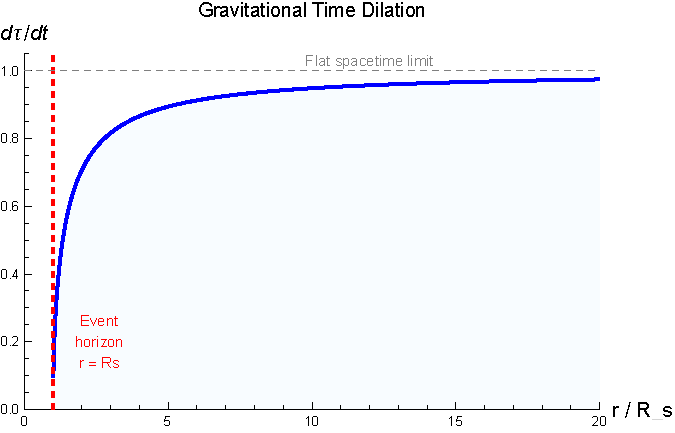
\includegraphics[width=0.65\textwidth]{../Figures/01c_Schwarzschild/time_dilation.pdf}
    \caption{Gravitational time dilation factor $d\tau/dt = \sqrt{1 - R_S/r}$
    as a function of $r/R_S$.  Clocks near the horizon ($r \to R_S$) are
    dramatically slowed.  Far from the mass ($r \gg R_S$), the factor
    approaches unity (flat spacetime).}
    \label{fig:time_dilation}
\end{figure}


% =====================================================================
\section{Gravitational Redshift}
\label{sec:gravitational_redshift}

A photon emitted at radius $r_{\mathrm{em}}$ with frequency
$\nu_{\mathrm{em}}$ is observed at $r_{\mathrm{obs}} \to \infty$ with
frequency:
\begin{equation}
    \frac{\nu_{\mathrm{obs}}}{\nu_{\mathrm{em}}}
    = \frac{\sqrt{1 - R_S/r_{\mathrm{em}}}}{\sqrt{1 - R_S/r_{\mathrm{obs}}}}
    \xrightarrow{r_{\mathrm{obs}} \to \infty}
    \sqrt{1 - \frac{R_S}{r_{\mathrm{em}}}} \,.
    \label{eq:grav_redshift}
\end{equation}
Since $\nu_{\mathrm{obs}} < \nu_{\mathrm{em}}$, the photon is
\textbf{redshifted} as it climbs out of the gravitational potential well.
The gravitational redshift parameter is:
\begin{equation}
    z_{\mathrm{grav}} = \frac{\nu_{\mathrm{em}}}{\nu_{\mathrm{obs}}} - 1
    = \left(1 - \frac{R_S}{r_{\mathrm{em}}}\right)^{-1/2} - 1 \,.
    \label{eq:grav_redshift_z}
\end{equation}
In the weak-field limit ($R_S/r \ll 1$): $z_{\mathrm{grav}} \approx GM/(rc^2)$
(Congdon \& Keeton eq.~3.63).

\begin{figure}[ht]
    \centering
    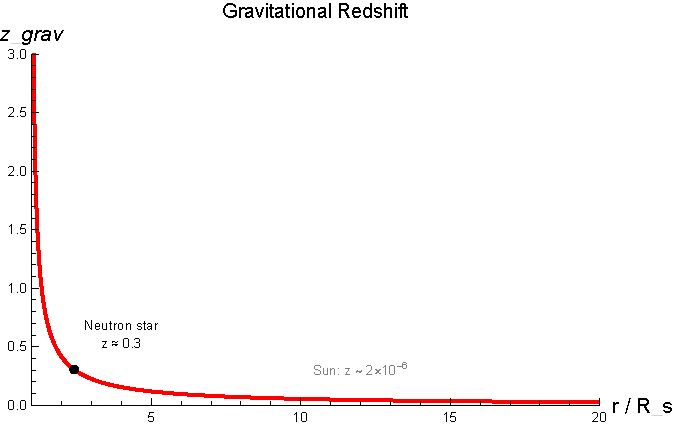
\includegraphics[width=0.65\textwidth]{../Figures/01c_Schwarzschild/gravitational_redshift.pdf}
    \caption{Gravitational redshift $z_{\mathrm{grav}}$ as a function of
    emission radius $r/R_S$.  The redshift diverges at the horizon.  The
    black dot marks a typical neutron star ($r/R_S \approx 2.4$,
    $z \approx 0.3$).  For the Sun, $z \sim 10^{-6}$.}
    \label{fig:grav_redshift}
\end{figure}

\begin{remark}
The gravitational redshift was one of the three classical tests of GR
proposed by Einstein, along with the perihelion precession of Mercury
and the bending of light.  It has been measured to high precision using
atomic clocks at different altitudes (e.g., Pound--Rebka experiment, 1959;
GPS satellite corrections).
\end{remark}


% =====================================================================
\section{The Event Horizon and Singularities}
\label{sec:event_horizon}

The Schwarzschild metric has two apparent singularities: at $r = 0$ and
at $r = R_S$.  Their nature is quite different (Carroll Sec.~5.3):

\paragraph{$r = R_S$ (coordinate singularity).}
The metric components diverge, but this is a \textit{coordinate artifact}.
The curvature remains finite, and the geometry is perfectly smooth.  In
appropriate coordinates (e.g., Eddington--Finkelstein or Kruskal--Szekeres),
the metric is regular at $r = R_S$.  However, $r = R_S$ is the
\textbf{event horizon}: once a particle crosses it, it can never return.

\paragraph{$r = 0$ (true singularity).}
This is a genuine physical singularity where the curvature becomes infinite.
We can confirm this with a curvature invariant: the
\textbf{Kretschner scalar}:
\begin{equation}
    K = R_{\mu\nu\rho\sigma}\, R^{\mu\nu\rho\sigma}
    = \frac{12\, R_S^2}{r^6}
    = \frac{48\, G^2 M^2}{c^4\, r^6} \,.
    \label{eq:kretschner}
\end{equation}
This diverges as $r \to 0$ but is finite at $r = R_S$, confirming that
only $r = 0$ is a true singularity.  We verify eq.~\eqref{eq:kretschner}
in \mathlink{01c_Schwarzschild/schwarzschild_metric.wl}{schwarzschild\_metric.wl}.


% =====================================================================
\section{Inside the Event Horizon: The Coordinate Swap}
\label{sec:dg_inside_horizon}

The Schwarzschild metric~\eqref{eq:schwarzschild_metric} describes
spacetime outside a spherical mass, but it also has something startling
to say about the region $r < R_S$.  Understanding this interior, even
briefly, sharpens our physical intuition about what the Schwarzschild
radius really means.

% ---------------------------------------------------------------------
\subsection{The Signature Flip}
\label{sec:dg_signature_flip}

Recall the Schwarzschild line element:
\[
    ds^2 = -\!\left(1 - \frac{R_S}{r}\right) c^2\, dt^2
    + \left(1 - \frac{R_S}{r}\right)^{-1} dr^2
    + r^2\, d\Omega^2 \,.
\]
Outside the horizon ($r > R_S$), the factor $f(r) \equiv 1 - R_S/r$ is
positive, so $g_{tt} < 0$ (timelike) and $g_{rr} > 0$ (spacelike).

Inside the horizon ($r < R_S$), this factor becomes \emph{negative}:
$f(r) < 0$.  Consequently:
\begin{itemize}[nosep]
    \item $g_{tt} = -f(r)\,c^2 > 0$ --- the $t$ direction is now
          \textbf{spacelike}.
    \item $g_{rr} = f(r)^{-1} < 0$ --- the $r$ direction is now
          \textbf{timelike}.
\end{itemize}
The roles of $r$ and $t$ have swapped.  Inside the horizon, $r$ is a
time coordinate and $t$ is a space coordinate.

% ---------------------------------------------------------------------
\subsection{Physical Meaning: The Singularity Is a Moment in Time}
\label{sec:dg_singularity_time}

Since $r$ is timelike inside the horizon, decreasing $r$ is the
\emph{future direction}.  Every future-directed worldline must have
$dr < 0$; the singularity at $r = 0$ is not a place you can steer
away from --- it is a \emph{moment in time} that all interior
observers inevitably reach.

\begin{remark}
You can no more avoid the singularity at $r = 0$ (once inside the
horizon) than you can avoid next Tuesday.  This is the precise sense
in which a black hole traps everything: it is not that the singularity
pulls you toward a point in space, but that the future itself points
toward $r = 0$.
\end{remark}

% ---------------------------------------------------------------------
\subsection{Why Nothing Escapes: Tilting Light Cones}
\label{sec:dg_light_cones}

For radial null rays ($ds^2 = 0$, $d\Omega = 0$) in Schwarzschild
coordinates:
\begin{equation}
    \frac{dr}{dt} = \pm\, c\left(1 - \frac{R_S}{r}\right) .
    \label{eq:radial_null}
\end{equation}
Outside the horizon, the two signs give outgoing ($+$) and ingoing ($-$)
light rays.  At $r = R_S$, both solutions give $dr/dt = 0$: light
``stands still'' in these coordinates (a coordinate effect, not a
physical one).

For $r < R_S$, the factor $(1 - R_S/r)$ is negative, so
$dr/dt$ has the \emph{same sign} for both solutions --- both
``outgoing'' and ``ingoing'' light rays have $dr < 0$ when $dt > 0$.
In other words, \textbf{all future-directed light cones point toward
smaller~$r$}.  No signal --- not even light --- can move to larger $r$
inside the horizon.

% ---------------------------------------------------------------------
\subsection{Eddington--Finkelstein Coordinates}
\label{sec:dg_eddington_finkelstein}

The pathological behavior at $r = R_S$ in Schwarzschild coordinates
is a coordinate artifact.  We can remove it by switching to
\textbf{ingoing Eddington--Finkelstein coordinates}.  Define the
advanced time coordinate:
\begin{equation}
    v = t + r_* \,, \qquad
    r_* = r + R_S \ln\!\left|\frac{r}{R_S} - 1\right| ,
    \label{eq:tortoise_and_v}
\end{equation}
where $r_*$ is the \textbf{tortoise coordinate} (Carroll eq.~5.58).
In terms of $(v, r, \theta, \phi)$, the Schwarzschild line element
becomes (Carroll eq.~5.60):
\begin{equation}
    \boxed{
    ds^2 = -\!\left(1 - \frac{R_S}{r}\right) c^2\, dv^2
    + 2c\, dv\, dr + r^2\, d\Omega^2
    }
    \label{eq:eddington_finkelstein}
\end{equation}
This metric is manifestly regular at $r = R_S$: every component is
finite and the determinant is nonzero.  The horizon is simply the
surface where outgoing light rays have $dr/dv = 0$; ingoing rays cross
it smoothly.

\begin{remark}
The Eddington--Finkelstein form makes it transparent that the event
horizon is a \emph{one-way membrane}: ingoing light ($dv > 0$,
$dr < 0$) crosses the horizon without incident, while outgoing light
at $r = R_S$ remains at $r = R_S$ forever.
\end{remark}

% ---------------------------------------------------------------------
\subsection{Relevance to Gravitational Lensing}
\label{sec:dg_interior_relevance}

\begin{remark}
For gravitational lensing, we work exclusively in the region
$r \gg R_S$ --- far outside the event horizon.  Galaxy-mass lenses
have $R_S \sim 0.1$ pc, while lensing occurs at scales of kiloparsecs.
The black hole interior is therefore not directly relevant to lensing
calculations.  Nevertheless, understanding the interior clarifies
\emph{why} the Schwarzschild radius is special (it is where light
cones tip over) and deepens physical intuition about the boundary
conditions of the exterior solution.
\end{remark}


% =====================================================================
\section{The Weak-Field Limit}
\label{sec:weak_field}

For $r \gg R_S$, the Schwarzschild metric reduces to the \textbf{weak-field}
form (Congdon \& Keeton eq.~3.71):
\begin{equation}
    ds^2 \approx -\left(1 + \frac{2\Phi}{c^2}\right) c^2 dt^2
    + \left(1 - \frac{2\Phi}{c^2}\right)
    \bigl[dr^2 + r^2\, d\Omega^2\bigr] \,,
    \label{eq:weak_field}
\end{equation}
where $\Phi = -GM/r$ is the Newtonian gravitational potential.  This
form is valid for \textit{any} weak gravitational field, not just the
Schwarzschild case, and will be the starting point for deriving the
deflection angle of light in Module~2.

\begin{remark}
The weak-field metric~\eqref{eq:weak_field} has an important feature:
the spatial part is modified by a factor $(1 - 2\Phi/c^2)$ as well as
the time part.  This means that gravity affects both the \textit{rate}
of clocks (time dilation) and the \textit{curvature of space}.
Both effects contribute equally to the bending of light --- this is why
GR gives twice the Newtonian deflection angle.
\end{remark}


% =====================================================================
\section{Isotropic Coordinates}
\label{sec:isotropic_coords}

The standard Schwarzschild coordinates $(t, r, \theta, \phi)$ have
an important asymmetry: the radial and angular parts of the spatial
metric carry \textit{different} factors.  In
eq.~\eqref{eq:schwarzschild_metric}, the $dr^2$ term is multiplied by
$(1 - R_S/r)^{-1}$ while the angular part $r^2\,d\Omega^2$ has no such
factor.  The spatial part of the Schwarzschild metric is therefore
\textit{not} conformally flat --- it is not proportional to the
flat-space metric $dr^2 + r^2\,d\Omega^2$.

We can remedy this by introducing \textbf{isotropic coordinates}, in
which the spatial metric \textit{is} conformally flat.

\subsection{The Isotropic Radial Coordinate}

Define a new radial coordinate $\rho$ via:
\begin{equation}
    r = \rho\left(1 + \frac{R_S}{4\rho}\right)^{\!2} .
    \label{eq:isotropic_r}
\end{equation}
This transformation is invertible for $r > R_S$ (i.e., outside the
event horizon), with the inverse
$\rho = \tfrac{1}{2}(r - R_S/2 + \sqrt{r^2 - r\,R_S})$.

\subsection{The Schwarzschild Metric in Isotropic Form}

In the coordinates $(t, \rho, \theta, \phi)$, the Schwarzschild
metric becomes:
\begin{equation}
    \boxed{
    ds^2 = -\left(\frac{1 - R_S/(4\rho)}{1 + R_S/(4\rho)}\right)^{\!2}
    c^2\, dt^2
    + \left(1 + \frac{R_S}{4\rho}\right)^{\!4}
    \bigl(d\rho^2 + \rho^2\, d\Omega^2\bigr)
    }
    \label{eq:schwarzschild_isotropic}
\end{equation}
The crucial feature is that the spatial part is now proportional to
the \textit{flat-space metric} $d\rho^2 + \rho^2\,d\Omega^2$ ---
the spatial geometry is \textbf{conformally flat}.  The single
conformal factor $(1 + R_S/(4\rho))^4$ multiplies all three spatial
directions equally, hence the name ``isotropic.''

\subsection{Weak-Field Expansion}

To first order in $R_S/\rho$ (the weak-field regime $\rho \gg R_S$),
the isotropic metric reduces to:
\begin{equation}
    ds^2 \approx -\left(1 - \frac{R_S}{2\rho}\right) c^2\, dt^2
    + \left(1 + \frac{R_S}{2\rho}\right)
    \bigl(d\rho^2 + \rho^2\, d\Omega^2\bigr) .
    \label{eq:isotropic_weak_field}
\end{equation}
Since $R_S = 2GM/c^2$, we have $R_S/(2\rho) = GM/(\rho\, c^2) =
-\Phi/c^2$ where $\Phi = -GM/\rho$ is the Newtonian potential.
Equation~\eqref{eq:isotropic_weak_field} is therefore:
\begin{equation}
    ds^2 \approx -\left(1 + \frac{2\Phi}{c^2}\right) c^2\, dt^2
    + \left(1 - \frac{2\Phi}{c^2}\right)
    \bigl(d\rho^2 + \rho^2\, d\Omega^2\bigr) ,
    \label{eq:isotropic_newtonian}
\end{equation}
which is precisely the weak-field metric~\eqref{eq:weak_field} with
$r$ replaced by $\rho$.  (In the weak-field regime, $r$ and $\rho$
agree to leading order.)

\subsection{Connection to the Linearized Gravity Formalism}

This result provides the explicit \textbf{bridge} between the exact
Schwarzschild solution (this module) and the linearized gravity
approach (Module~1e).  In Module~1e, the weak-field metric is derived
from first principles as a perturbation of flat spacetime:
$g_{\mu\nu} = \eta_{\mu\nu} + h_{\mu\nu}$ with
$h_{00} = -2\Phi/c^2$ and $h_{ij} = -2\Phi/c^2\,\delta_{ij}$.
The isotropic form~\eqref{eq:isotropic_newtonian} shows that the
Schwarzschild solution, when expanded to first order, reproduces
exactly this linearized metric.  The two descriptions --- exact
solution in curved coordinates, and perturbation theory in nearly
flat coordinates --- describe the \textit{same physics} in different
coordinate systems.

\begin{remark}
The isotropic form makes the connection to the parameterized
post-Newtonian (PPN) formalism and the factor-of-2 in light
deflection transparent.  In eq.~\eqref{eq:isotropic_newtonian}, both
$h_{00} = -2\Phi/c^2$ (time perturbation) and
$h_{ij} = -2\Phi/c^2\,\delta_{ij}$ (space perturbation) are
proportional to $R_S/\rho$, confirming that the time and space
perturbations are \textit{equal}.  In the PPN formalism, this
equality corresponds to $\gamma_{\mathrm{PPN}} = 1$, which is the GR
prediction.  As we saw in the weak-field limit discussion, this equal
contribution of time and space curvature is precisely why GR predicts
\textit{twice} the Newtonian deflection angle for light.
\end{remark}


% =====================================================================
\section{Schwarzschild Radius for Astrophysical Objects}
\label{sec:RS_examples}

\begin{center}
\begin{tabular}{llll}
\toprule
\textbf{Object} & \textbf{Mass} & $R_S$ & \textbf{Actual Radius} \\
\midrule
Earth   & $6 \times 10^{24}$ kg  & 8.9 mm     & 6371 km \\
Sun     & $2 \times 10^{30}$ kg  & 3.0 km     & $7 \times 10^5$ km \\
Neutron star & $1.4\,\Msun$      & 4.1 km     & $\sim 10$ km \\
SgrA*   & $4 \times 10^6\,\Msun$ & $1.2 \times 10^7$ km & --- (black hole) \\
Galaxy ($10^{12}\,\Msun$) & $10^{12}\,\Msun$ & $3 \times 10^{12}$ km & --- \\
\bottomrule
\end{tabular}
\end{center}

For a galaxy-mass lens ($M \sim 10^{12}\, \Msun$), $R_S \sim 0.1$ pc ---
far smaller than the galaxy itself.  This confirms that the weak-field
limit is appropriate for gravitational lensing by galaxies.


% =====================================================================
\section{Embedding Diagram: Flamm's Paraboloid}
\label{sec:flamm}

To visualize the spatial curvature of the Schwarzschild geometry, we can
embed the equatorial ($\theta = \pi/2$) spatial slice in 3D Euclidean space.
At constant time $t$, the spatial metric on the equatorial plane is:
\begin{equation}
    dl^2 = \left(1 - \frac{R_S}{r}\right)^{-1} dr^2 + r^2\, d\phi^2 \,.
    \label{eq:equatorial_metric}
\end{equation}
Embedding this as a surface of revolution $z(r)$ in cylindrical coordinates
$(r, \phi, z)$ where $dl^2 = (1 + z'^2) dr^2 + r^2 d\phi^2$, we find:
\begin{equation}
    z(r) = 2\sqrt{R_S}\,\sqrt{r - R_S} \,,
    \label{eq:flamm}
\end{equation}
which is \textbf{Flamm's paraboloid} (Figure~\ref{fig:flamm}).

\begin{figure}[ht]
    \centering
    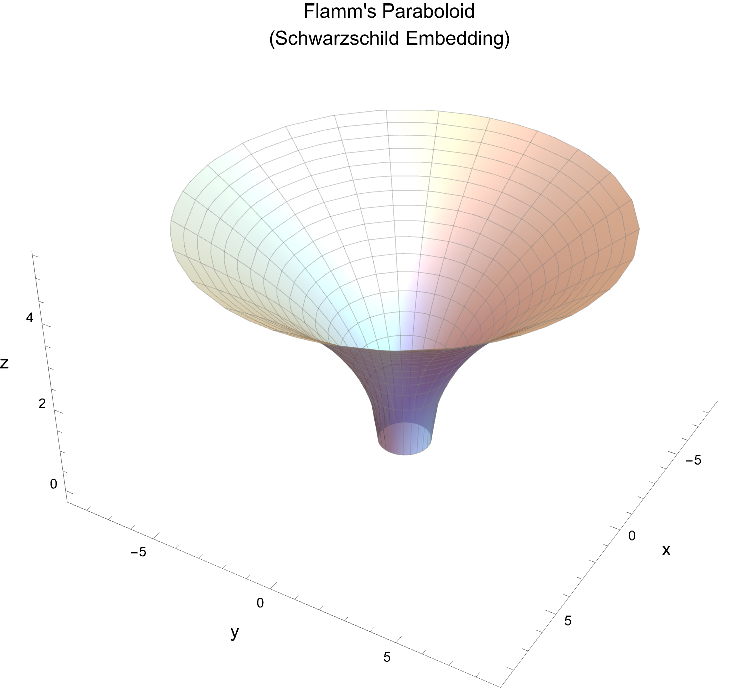
\includegraphics[width=0.7\textwidth]{../Figures/01c_Schwarzschild/flamm_paraboloid.pdf}
    \caption{Flamm's paraboloid: the equatorial spatial geometry of the
    Schwarzschild spacetime embedded in 3D Euclidean space.  The throat
    at $r = R_S$ represents the event horizon.  The surface curves more
    steeply near the throat, visualizing the spatial curvature caused by
    gravity.  An interactive version is in
    \texttt{gravitational\_redshift.nb}.}
    \label{fig:flamm}
\end{figure}


% =====================================================================
\section{Summary}
\label{sec:schwarzschild_summary}

\begin{itemize}
    \item The Schwarzschild metric is the unique spherically symmetric
          vacuum solution (Birkhoff's theorem).
    \item It is parameterized by a single quantity: the mass $M$
          (or equivalently the Schwarzschild radius $R_S = 2GM/c^2$).
    \item Gravitational time dilation: clocks run slower in stronger
          gravitational fields; $d\tau = \sqrt{1 - R_S/r}\, dt$.
    \item Gravitational redshift: photons lose energy climbing out
          of a potential well.
    \item $r = R_S$ is a coordinate singularity (event horizon);
          $r = 0$ is a true curvature singularity.
    \item The weak-field limit
          ($ds^2 \approx -(1 + 2\Phi/c^2)c^2 dt^2 + (1 - 2\Phi/c^2) d\ell^2$)
          will be the foundation for light deflection in Module~2.
\end{itemize}


% =====================================================================
\section{Problems}
\label{sec:schwarzschild_problems}

\begin{exercise}
\label{ex:verify_vacuum}
Using the reusable functions from Module~1b
(\mathlink{01b_Differential_Geometry/christoffel_symbols.wl}{christoffel\_symbols.wl}),
verify that the Schwarzschild metric~\eqref{eq:schwarzschild_metric}
satisfies $R_{\mu\nu} = 0$.
\end{exercise}

\begin{exercise}
\label{ex:kretschner}
Compute the Kretschner scalar $K = R_{\mu\nu\rho\sigma}R^{\mu\nu\rho\sigma}$
for the Schwarzschild metric and show that $K = 12\,R_S^2/r^6$.
Verify that $K$ is finite at $r = R_S$ but diverges at $r = 0$.
\end{exercise}

\begin{exercise}
\label{ex:schwarzschild_radii}
Compute the Schwarzschild radius for:
\begin{enumerate}[label=(\alph*)]
    \item The Earth ($M = 5.97 \times 10^{24}$ kg)
    \item The Sun ($M = 1.99 \times 10^{30}$ kg)
    \item A typical galaxy lens ($M = 10^{12}\, \Msun$)
\end{enumerate}
In each case, compare $R_S$ to the physical size of the object.
\end{exercise}

\begin{exercise}
\label{ex:grav_redshift_calc}
A photon is emitted from the surface of a neutron star ($M = 1.4\,\Msun$,
$R = 10$ km).
\begin{enumerate}[label=(\alph*)]
    \item Compute the gravitational redshift $z_{\mathrm{grav}}$.
    \item By what fraction is the photon's wavelength increased by the time
          it reaches a distant observer?
    \item Compare to the redshift from the surface of the Sun.
\end{enumerate}
\end{exercise}

\begin{exercise}
\label{ex:flamm_derive}
Derive the Flamm's paraboloid embedding~\eqref{eq:flamm} by embedding the
equatorial spatial slice of the Schwarzschild geometry in 3D Euclidean
space with cylindrical coordinates $(r, \phi, z)$.
\end{exercise}

% =============================================================================
% Module 1d: Geodesics and Orbits in Schwarzschild Spacetime
% =============================================================================
% Sources: Carroll Ch. 5 (Secs. 5.4--5.5), Congdon & Keeton Ch. 3.3.3
% Mathematica: ../Mathematica/01d_Geodesics_Orbits/
% =============================================================================

\chapter{Geodesics and Orbits in Schwarzschild Spacetime}
\label{ch:geodesics_orbits}

\begin{quote}
\textit{Together the conserved quantities $E$ and $L$ provide a convenient way
to understand the orbits of particles in the Schwarzschild geometry.}
\hfill --- Sean Carroll, \textit{Spacetime and Geometry}
\end{quote}

\noindent
In Module~1c we derived the Schwarzschild metric.  Now we ask: how do
particles and light \textit{move} in this spacetime?  The answer comes from
the geodesic equation, which we reduce to a one-dimensional effective
potential problem using Killing vectors and conservation laws.  This
module derives the effective potential for massive and massless particles,
identifies the key features (ISCO, photon sphere), and culminates in
Mercury's perihelion precession --- one of the three classical tests of GR.

\medskip
\noindent
\textbf{Companion Mathematica files:}
\begin{itemize}[nosep]
    \item \mathlink{01d_Geodesics_Orbits/geodesic_equation.wl}{geodesic\_equation.wl}
          --- symbolic derivation of the geodesic equations, conserved
          quantities, effective potential, ISCO, photon sphere, and
          perihelion precession formula
    \item \mathlink{01d_Geodesics_Orbits/effective_potential.nb}{effective\_potential.nb}
          --- interactive plots of effective potential with sliders for
          $L$ and $\epsilon$; orbit integration; precessing ellipses
\end{itemize}


% =====================================================================
\section{Killing Vectors and Conservation Laws}
\label{sec:killing_vectors}

The Schwarzschild metric is independent of both $t$ and $\phi$, which
means it possesses two \textbf{Killing vectors} (Carroll Sec.~5.4):
\begin{equation}
    K^\mu = (\partial_t)^\mu = (1, 0, 0, 0) \quad \text{(time translation)},
    \label{eq:killing_t}
\end{equation}
\begin{equation}
    R^\mu = (\partial_\phi)^\mu = (0, 0, 0, 1) \quad \text{(axial rotation)}.
    \label{eq:killing_phi}
\end{equation}
For any geodesic $x^\mu(\lambda)$, the quantity $K_\mu\, dx^\mu/d\lambda$
is conserved along the path (Carroll eq.~5.54).  Lowering the index with
the metric gives the two conserved quantities (Carroll eqs.~5.61--5.62):
\begin{equation}
    \boxed{
    E = \left(1 - \frac{R_S}{r}\right) \frac{dt}{d\lambda}
    }
    \label{eq:conserved_E}
\end{equation}
\begin{equation}
    \boxed{
    L = r^2 \frac{d\phi}{d\lambda}
    }
    \label{eq:conserved_L}
\end{equation}
For massive particles ($\lambda = \tau$), $E$ and $L$ are the conserved
energy and angular momentum \textit{per unit mass}.  For photons, they are
the energy and angular momentum of the photon (up to normalization of the
affine parameter).

Additionally, spherical symmetry allows us to restrict all orbits to the
equatorial plane $\theta = \pi/2$ without loss of generality (Carroll
eq.~5.56).


% =====================================================================
\section{The Effective Potential}
\label{sec:effective_potential}

The normalization condition for the four-velocity gives
(Carroll eq.~5.63):
\begin{equation}
    -\left(1 - \frac{R_S}{r}\right)\left(\frac{dt}{d\lambda}\right)^2
    + \left(1 - \frac{R_S}{r}\right)^{-1}\left(\frac{dr}{d\lambda}\right)^2
    + r^2\left(\frac{d\phi}{d\lambda}\right)^2 = -\epsilon \,,
    \label{eq:normalization}
\end{equation}
where $\epsilon = 1$ for massive particles (timelike geodesics) and
$\epsilon = 0$ for photons (null geodesics).

Substituting the conserved quantities~\eqref{eq:conserved_E}
and~\eqref{eq:conserved_L}, we obtain a radial equation
(Carroll eq.~5.64):
\begin{equation}
    \frac{1}{2}\left(\frac{dr}{d\lambda}\right)^2 + V_{\mathrm{eff}}(r)
    = \mathcal{E} \,,
    \label{eq:radial_equation}
\end{equation}
where the \textbf{effective potential} is (Carroll eq.~5.66;
Congdon \& Keeton eq.~3.80):
\begin{equation}
    \boxed{
    V_{\mathrm{eff}}(r) = -\epsilon\,\frac{GM}{r}
    + \frac{L^2}{2r^2}
    - \frac{GML^2}{c^2 r^3}
    }
    \label{eq:effective_potential}
\end{equation}
and $\mathcal{E} = \half(E^2 - \epsilon c^2)$ is the effective ``energy.''

\begin{remark}
The three terms in $V_{\mathrm{eff}}$ have clear physical interpretations:
\begin{enumerate}[nosep]
    \item $-\epsilon\, GM/r$: the Newtonian gravitational potential
          (absent for photons since $\epsilon = 0$)
    \item $L^2/(2r^2)$: the centrifugal barrier (identical to Newtonian
          mechanics)
    \item $-GML^2/(c^2 r^3)$: the \textbf{GR correction} --- this term
          has no Newtonian analogue and is responsible for all the
          distinctive features of relativistic orbits
\end{enumerate}
The GR term is attractive at small $r$, which means the centrifugal
barrier can be overcome --- this is why particles can spiral into black
holes, which is impossible in Newtonian gravity.
\end{remark}

\begin{figure}[ht]
    \centering
    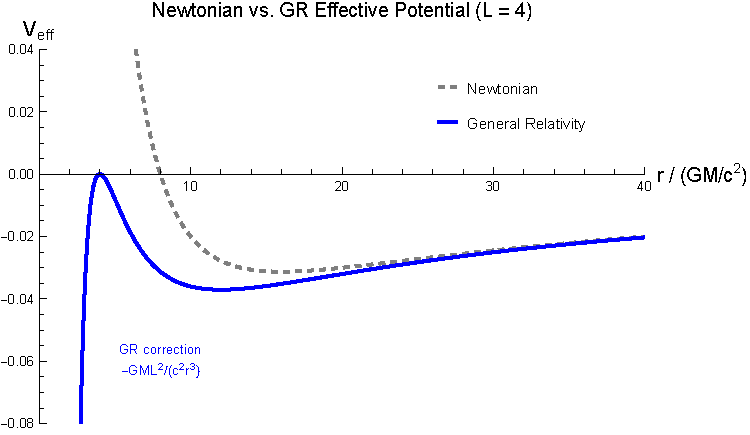
\includegraphics[width=0.75\textwidth]{../Figures/01d_Geodesics_Orbits/newtonian_vs_gr.pdf}
    \caption{Comparison of Newtonian (dashed) and GR (solid) effective
    potentials for a massive particle with $L = 4\,GM/c$.  The GR correction
    term $\propto 1/r^3$ pulls the potential down at small $r$, allowing
    particles to plunge past the centrifugal barrier.
    (cf.\ Carroll Figs.~5.4 and 5.5)}
    \label{fig:newtonian_vs_gr}
\end{figure}


% =====================================================================
\section{Circular Orbits and the ISCO}
\label{sec:circular_orbits}

Circular orbits occur at extrema of the effective potential:
$dV_{\mathrm{eff}}/dr = 0$.  For massive particles ($\epsilon = 1$),
this gives (Carroll eq.~5.68):
\begin{equation}
    GM r_c^2 - L^2 r_c + 3GML^2/c^2 = 0 \,.
    \label{eq:circular_condition}
\end{equation}
The two solutions are (Carroll eq.~5.71):
\begin{equation}
    r_\pm = \frac{L^2}{2GM}
    \left(1 \pm \sqrt{1 - \frac{12G^2M^2}{L^2 c^2}}\right) \,.
    \label{eq:circular_radii}
\end{equation}

\begin{itemize}
    \item $r_+$ (outer): \textbf{stable} circular orbit (minimum of $V_{\mathrm{eff}}$)
    \item $r_-$ (inner): \textbf{unstable} circular orbit (maximum of $V_{\mathrm{eff}}$)
\end{itemize}

Real solutions require $L^2 \geq 12\,G^2M^2/c^2$, i.e.,
$L \geq 2\sqrt{3}\,GM/c$ (Carroll eq.~5.73).  The minimum stable circular
orbit occurs when $r_+ = r_-$, giving the \textbf{innermost stable
circular orbit (ISCO)} (Carroll eq.~5.74; Congdon \& Keeton eq.~3.84):
\begin{equation}
    \boxed{r_{\mathrm{ISCO}} = \frac{6GM}{c^2} = 3\, R_S}
    \label{eq:ISCO}
\end{equation}

\begin{remark}
The ISCO is a fundamental scale in black hole astrophysics.  Accreting
matter in a thin disk spirals inward until it reaches the ISCO, then
plunges into the black hole.  The ISCO radius determines the
efficiency of energy extraction from accretion and the inner edge of
accretion disks observed in X-ray binaries and active galactic nuclei.
\end{remark}


% =====================================================================
\section{The Photon Sphere}
\label{sec:photon_sphere}

For photons ($\epsilon = 0$), the effective potential simplifies to
(Congdon \& Keeton eq.~3.86):
\begin{equation}
    V_{\mathrm{eff}}^{\mathrm{photon}}(r) = \frac{L^2}{2r^2}
    - \frac{GML^2}{c^2 r^3} \,.
    \label{eq:Veff_photon}
\end{equation}
Setting $dV_{\mathrm{eff}}/dr = 0$ gives a single circular orbit
(Carroll eq.~5.70; Congdon \& Keeton eq.~3.84 with $\ell_{\mathrm{crit}}$):
\begin{equation}
    \boxed{r_{\mathrm{photon}} = \frac{3GM}{c^2} = \frac{3}{2}\, R_S}
    \label{eq:photon_sphere}
\end{equation}
This is an \textit{unstable} circular orbit --- any perturbation causes
the photon to either escape to infinity or spiral into the black hole.
Nevertheless, the photon sphere plays a key role in strong gravitational
lensing near black holes and is directly related to the ``photon ring''
observed by the Event Horizon Telescope.


% =====================================================================
\section{Effective Potential: Newtonian vs.\ GR}
\label{sec:veff_comparison}

The key qualitative differences between Newtonian and GR effective
potentials are:

\begin{center}
\begin{tabular}{lcc}
\toprule
\textbf{Feature} & \textbf{Newtonian} & \textbf{GR} \\
\midrule
Centrifugal barrier & Diverges as $r \to 0$ & Overcome at small $r$ \\
ISCO & None (stable at any $r$) & $r = 3R_S$ \\
Photon orbits & None & Unstable at $r = 3R_S/2$ \\
Plunge orbits & Impossible & Possible for $r < r_{\mathrm{ISCO}}$ \\
\bottomrule
\end{tabular}
\end{center}

\begin{figure}[ht]
    \centering
    \begin{subfigure}[b]{0.48\textwidth}
        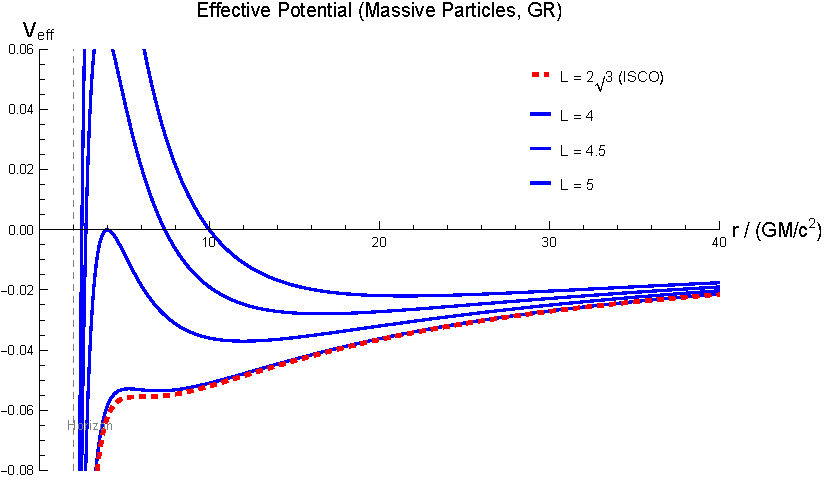
\includegraphics[width=\textwidth]{../Figures/01d_Geodesics_Orbits/effective_potential_massive.pdf}
        \caption{Massive particles ($\epsilon = 1$)}
    \end{subfigure}
    \hfill
    \begin{subfigure}[b]{0.48\textwidth}
        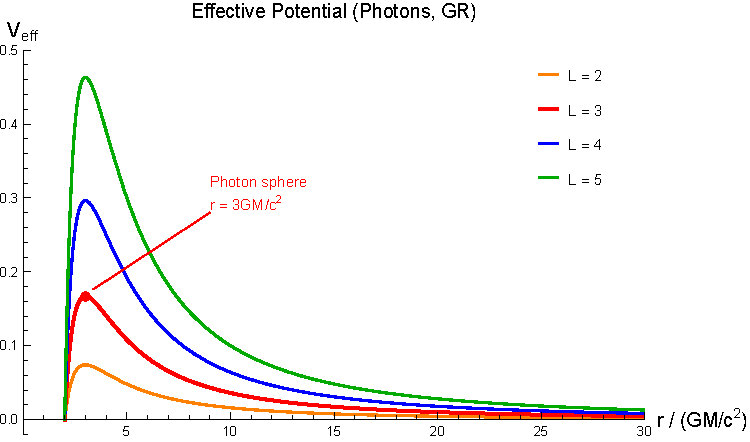
\includegraphics[width=\textwidth]{../Figures/01d_Geodesics_Orbits/effective_potential_photon.pdf}
        \caption{Photons ($\epsilon = 0$)}
    \end{subfigure}
    \caption{GR effective potentials for several values of angular momentum
    $L$ (in $GM/c$ units).  \textbf{Left:} For massive particles, the red
    dashed curve shows $L = L_{\mathrm{ISCO}} = 2\sqrt{3}\,GM/c$, where
    the stable and unstable circular orbits merge.  \textbf{Right:} For
    photons, the potential always has a maximum at $r = 3GM/c^2$ (the photon
    sphere).  Interactive versions in
    \texttt{effective\_potential.nb}.}
    \label{fig:effective_potentials}
\end{figure}


% =====================================================================
\section{Perihelion Precession}
\label{sec:perihelion_precession}

In Newtonian gravity, bound orbits are perfect ellipses that close on
themselves.  In GR, the extra $-GML^2/(c^2 r^3)$ term in the effective
potential causes the orbit to \textit{precess}: the perihelion (point of
closest approach) advances by a small angle each orbit.

Following Carroll Sec.~5.5 and using the substitution $x = L^2/(GMr)$,
the orbit equation becomes (Carroll eq.~5.79):
\begin{equation}
    \frac{d^2 x}{d\phi^2} + x = 1 + \frac{3G^2M^2}{L^2 c^2}\, x^2 \,.
    \label{eq:orbit_equation}
\end{equation}
The last term is the GR correction.  Treating it as a perturbation
($x = x_0 + x_1$, with $x_0 = 1 + e\cos\phi$ the Keplerian solution),
one finds the accumulated precession per orbit
(Carroll eq.~5.92; Congdon \& Keeton eq.~3.95):
\begin{equation}
    \boxed{
    \Delta\phi = \frac{6\pi G M}{c^2 a(1 - e^2)}
    = \frac{6\pi G M}{L^2 / (GM)}
    }
    \label{eq:perihelion_precession}
\end{equation}
where $a$ is the semi-major axis and $e$ the eccentricity.

For Mercury (Carroll eq.~5.96):
\begin{equation}
    \Delta\phi_{\mathrm{Mercury}} = 5.01 \times 10^{-7}~\text{rad/orbit}
    = 0.103''\text{/orbit} = 43.0''\text{/century} \,.
    \label{eq:mercury_precession}
\end{equation}
This matched the previously unexplained 43~arcseconds/century discrepancy
in Mercury's orbit and was one of Einstein's first confirmations of GR.

\begin{figure}[ht]
    \centering
    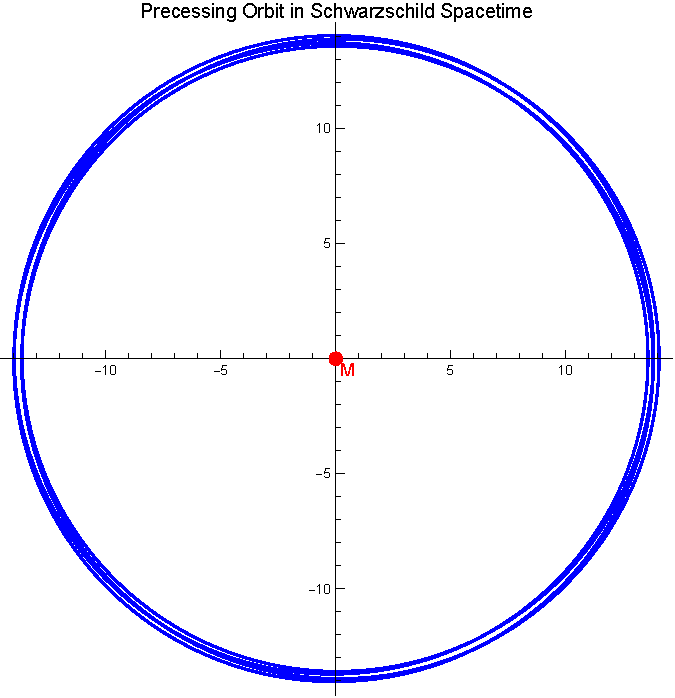
\includegraphics[width=0.55\textwidth]{../Figures/01d_Geodesics_Orbits/precessing_orbit.pdf}
    \caption{A precessing orbit in Schwarzschild spacetime, computed by
    numerically integrating the orbit equation.  The perihelion advances
    by a small angle each orbit, tracing out a rosette pattern.
    (cf.\ Carroll Fig.~5.6)}
    \label{fig:precessing_orbit}
\end{figure}


% =====================================================================
\section{Null Geodesics and the Deflection of Light (Preview)}
\label{sec:null_geodesics_preview}

For photons, the orbit equation (using $u = 1/r$) becomes
(Congdon \& Keeton eq.~3.87):
\begin{equation}
    \frac{d\phi}{dr} = \pm \frac{L}{r^2}
    \left[\frac{E^2}{c^2} - \frac{L^2}{r^2}\left(1 - \frac{R_S}{r}\right)
    \right]^{-1/2} \,.
    \label{eq:photon_orbit}
\end{equation}
A photon approaching a mass $M$ with impact parameter $b = cL/E$
(the perpendicular distance from the mass in the absence of deflection)
will be deflected by an angle (Congdon \& Keeton eq.~3.96):
\begin{equation}
    \hat{\alpha} = \frac{4GM}{c^2 b} \,,
    \label{eq:deflection_preview}
\end{equation}
in the weak-field limit ($b \gg R_S$).  This is \textit{twice} the
Newtonian prediction and was confirmed by Eddington's 1919 solar eclipse
observations.

The full derivation of the deflection angle is the subject of Module~2.
We mention it here because the effective potential framework makes it
clear \textit{why} light bends: photons follow null geodesics of the
curved Schwarzschild spacetime, and the GR correction term in the
effective potential deflects them more strongly than Newtonian gravity
would predict.


% =====================================================================
\section{Brief Overview: The Kerr Metric}
\label{sec:kerr_overview}

Real astrophysical black holes are not perfectly described by the
Schwarzschild solution because they \textit{rotate}.  The metric for a
rotating, axially symmetric black hole is the \textbf{Kerr metric},
discovered by Roy Kerr in 1963.  In Boyer--Lindquist coordinates, it
takes the form:
\begin{equation}
    ds^2 = -\left(1 - \frac{R_S r}{\Sigma}\right) c^2 dt^2
    - \frac{2R_S r a \sin^2\theta}{\Sigma}\, c\, dt\, d\phi
    + \frac{\Sigma}{\Delta}\, dr^2
    + \Sigma\, d\theta^2
    + \frac{A \sin^2\theta}{\Sigma}\, d\phi^2 \,,
    \label{eq:kerr_metric}
\end{equation}
where
\begin{align}
    \Sigma &= r^2 + a^2\cos^2\theta \,, &
    \Delta &= r^2 - R_S r + a^2 \,, &
    A &= (r^2 + a^2)^2 - a^2 \Delta \sin^2\theta \,,
    \label{eq:kerr_functions}
\end{align}
and $a = J/(Mc)$ is the \textbf{spin parameter} (angular momentum per
unit mass, with dimensions of length).  Note $0 \leq a \leq GM/c^2$
for a physical black hole.

Key features that differ from Schwarzschild:
\begin{itemize}
    \item \textbf{Frame dragging:} The $dt\,d\phi$ cross-term forces
          particles near the black hole to co-rotate.  This effect is
          absent in Schwarzschild.
    \item \textbf{Ergosphere:} The region $R_S/2 < r < (R_S + \sqrt{R_S^2 -
          4a^2\cos^2\theta})/2$ where even stationary observers must rotate
          with the black hole.
    \item \textbf{Spin-dependent ISCO:} The ISCO radius depends on the spin
          parameter and the direction of the orbit (prograde vs.\ retrograde).
          For a maximally spinning black hole ($a = GM/c^2$):
          $r_{\mathrm{ISCO}} = GM/c^2$ (prograde) vs.\
          $r_{\mathrm{ISCO}} = 9GM/c^2$ (retrograde), compared to
          $6GM/c^2$ for Schwarzschild.
    \item \textbf{Two horizons:}
          $r_\pm = GM/c^2 \pm \sqrt{(GM/c^2)^2 - a^2}$.
\end{itemize}

\begin{remark}
For gravitational lensing by galaxies and clusters, the Kerr metric is
not needed: the lensing effect is dominated by the total enclosed mass,
and the weak-field/thin-lens approximation (Module~1e and beyond) washes
out spin effects at the angular scales of interest.  However, Kerr lensing
is an active research topic for \textit{strong} lensing near individual
black holes --- for instance, the ``photon ring'' structure observed by
the Event Horizon Telescope, where frame-dragging produces asymmetric
brightness patterns.
\end{remark}


% =====================================================================
\section{Summary}
\label{sec:geodesics_summary}

\begin{itemize}
    \item Killing vectors ($\partial_t$, $\partial_\phi$) yield conserved
          energy $E$ and angular momentum $L$ along geodesics.
    \item The radial motion reduces to a 1D effective potential problem:
          $V_{\mathrm{eff}} = -\epsilon GM/r + L^2/(2r^2) - GML^2/(c^2 r^3)$.
    \item The GR correction term $\propto 1/r^3$ is responsible for:
          ISCO at $r = 3R_S$, photon sphere at $r = 3R_S/2$, perihelion
          precession, and enhanced light deflection.
    \item Mercury's perihelion precesses by 43 arcsec/century --- confirmed
          by observation and one of the first tests of GR.
    \item The Kerr metric generalizes Schwarzschild to rotating black holes
          (frame dragging, ergosphere, spin-dependent ISCO), but is not
          needed for galaxy/cluster-scale lensing.
\end{itemize}


% =====================================================================
\section{Problems}
\label{sec:geodesics_problems}

\begin{exercise}
\label{ex:derive_veff}
Starting from the normalization condition~\eqref{eq:normalization} and the
conserved quantities $E$ and $L$, derive the effective
potential~\eqref{eq:effective_potential} for massive particles
($\epsilon = 1$).  Show that in the Newtonian limit ($c \to \infty$,
$R_S \to 0$), it reduces to
$V_{\mathrm{eff}}^{\mathrm{Newton}} = -GM/r + L^2/(2r^2)$.
\end{exercise}

\begin{exercise}
\label{ex:isco_derivation}
Derive the ISCO radius by finding the value of $L$ for which the two
circular orbit solutions~\eqref{eq:circular_radii} coincide (i.e., the
discriminant vanishes).  Verify $r_{\mathrm{ISCO}} = 6GM/c^2 = 3R_S$.
\end{exercise}

\begin{exercise}
\label{ex:photon_sphere_derivation}
Show that the only circular photon orbit in the Schwarzschild spacetime is
at $r = 3GM/c^2 = 3R_S/2$, and that it is unstable (a maximum of
$V_{\mathrm{eff}}^{\mathrm{photon}}$).
\end{exercise}

\begin{exercise}
\label{ex:mercury_precession}
Compute the perihelion precession of Mercury using
eq.~\eqref{eq:perihelion_precession} with:
$M = M_\odot$, $a = 5.79 \times 10^{10}$~m, $e = 0.2056$.
Verify $\Delta\phi \approx 43''$/century (Mercury's orbital period is
87.97 days).
\end{exercise}

\begin{exercise}
\label{ex:orbit_integration}
Using the effective potential for massive particles with $L = 4GM/c$:
\begin{enumerate}[label=(\alph*)]
    \item Plot $V_{\mathrm{eff}}(r)$ and identify the stable circular
          orbit radius, the unstable circular orbit radius, and the
          ISCO.
    \item For a particle with $\mathcal{E}$ slightly above
          $V_{\mathrm{eff}}(r_+)$, describe qualitatively the type of
          orbit (bound precessing ellipse, scatter orbit, or plunge orbit).
\end{enumerate}
\end{exercise}


% =============================================================================
% Part II: Gravitational Lensing Theory
% =============================================================================
\part{Gravitational Lensing Theory}

% =============================================================================
% Module 2: Light Deflection in Curved Spacetime
% =============================================================================
% Sources: Carroll Ch. 5.5, Congdon & Keeton Ch. 3.4 (eqs. 3.87--3.96,
%          3.97--3.110), Narayan & Bartelmann Sec. 2.1
% Mathematica: ../Mathematica/02_Light_Deflection/
% =============================================================================

\chapter{Light Deflection in Curved Spacetime}
\label{ch:light_deflection}

\begin{quote}
\textit{The chief attraction of the theory lies in its logical completeness.
If a single one of the conclusions drawn from it proves wrong, it must be
given up; to modify it without destroying the whole structure seems to be
impossible.}
\hfill --- Albert Einstein, 1919
\end{quote}

\noindent
In Module~1d we derived the effective potential for geodesic motion in
Schwarzschild spacetime, and in Module~1e we obtained the deflection
angle $\alphahat = 4\Gnewton M / (\speedoflight^2 b)$ via the
weak-field / Born approximation, showing how the factor of 2 over
Newtonian gravity arises from the equal contributions of temporal and
spatial curvature.  Now we derive this same result rigorously from the
\textit{exact} null geodesic orbit equation in the full Schwarzschild
metric.  This is
the single most important result in gravitational lensing theory --- every
lens equation, every magnification formula, and every time delay expression
ultimately rests on it.

We also derive the Shapiro time delay, which provides the second
observable consequence of light propagation through a gravitational field,
and compute the deflection for several astrophysically relevant systems:
the Sun (Eddington's 1919 test), Jupiter, and a typical galaxy lens.

\medskip
\noindent
\textbf{Companion Mathematica files:}
\begin{itemize}[nosep]
    \item \mathlink{02_Light_Deflection/deflection_angle.wl}{deflection\_angle.wl}
          --- symbolic derivation of the deflection angle integral,
          weak-field expansion, numerical evaluation for Sun/Jupiter/galaxy,
          Shapiro delay, exact vs.\ approximate comparison, and figure generation
    \item \mathlink{02_Light_Deflection/deflection_geometry.nb}{deflection\_geometry.nb}
          --- interactive notebook: ray-bending geometry, sliders for~$M$
          and~$b$, exact vs.\ weak-field comparison with error percentage
\end{itemize}


% =====================================================================
\section{Introduction: Null Geodesics and the Deflection Problem}
\label{sec:deflection_intro}

Light follows \textbf{null geodesics} in curved spacetime: paths for which
$ds^2 = 0$ at every point.  In Module~1d we showed that for a photon in
the equatorial plane of the Schwarzschild metric, the conserved energy~$E$
and angular momentum~$L$ reduce the equations of motion to a single radial
equation (cf.\ eqs.~\ref{eq:conserved_E}--\ref{eq:conserved_L} and the
null geodesic orbit equation~\eqref{eq:photon_orbit} from Module~1d):
\begin{equation}
    \frac{d\phi}{dr} = \pm \frac{L}{r^2}
    \left[\frac{E^2}{\speedoflight^2}
    - \frac{L^2}{r^2}\!\left(1 - \frac{\RS}{r}\right)
    \right]^{-1/2} ,
    \label{eq:photon_orbit_eq}
\end{equation}
where $\RS = 2\Gnewton M / \speedoflight^2$ is the Schwarzschild radius
(Congdon \& Keeton eq.~3.87).

The physical setup is as follows.  A photon approaches a mass~$M$ from
infinity, reaches a distance of closest approach~$r_0$, and then escapes
back to infinity.  The total change in the azimuthal angle~$\phi$ is
$\Delta\phi$; in flat spacetime this would be~$\pi$ (a straight line), so
the \textbf{deflection angle} is
\begin{equation}
    \alphahat = \Delta\phi - \pi \,.
    \label{eq:deflection_def}
\end{equation}
Our goal in this chapter is to evaluate $\Delta\phi$ and show that, in the
weak-field limit,
\begin{equation}
    \boxed{
    \alphahat = \frac{4\Gnewton M}{\speedoflight^2\, b}
    }
    \label{eq:alphahat_main}
\end{equation}
where $b$ is the impact parameter.  This is the fundamental result of
gravitational lensing.


% =====================================================================
\section{Soldner's Newtonian Calculation (1801)}
\label{sec:soldner}

Before Einstein, Johann Georg von Soldner (1801) computed the deflection
of light using Newtonian gravity, treating a photon as a corpuscle of
mass~$m$ traveling at speed~$\speedoflight$.

\begin{remark}
Soldner's calculation predates general relativity by over a century.
It is both historically important and pedagogically useful: it gives
exactly \textit{half} the correct GR answer, and understanding
\textit{why} illuminates the role of spatial curvature.
\end{remark}

Consider a particle approaching a mass~$M$ on a hyperbolic trajectory with
velocity~$v_\infty = \speedoflight$ at infinity.  The Newtonian equations
of motion in polar coordinates yield the orbit equation
\begin{equation}
    r(\phi) = \frac{p}{1 + e\cos\phi} \,,
    \label{eq:newtonian_orbit}
\end{equation}
where $p = L^2/(GM)$ and $e = \sqrt{1 + 2\mathcal{E}L^2/(G^2 M^2)}$ is the
eccentricity (with $\mathcal{E} = \half \speedoflight^2$ for an unbound
particle at speed~$\speedoflight$).

The asymptotic directions correspond to $r \to \infty$, i.e.,
$\cos\phi = -1/e$.  The total angle swept is $\Delta\phi = \pi + 2\delta$,
where $\sin\delta = 1/e$.  For large impact parameter ($b \gg \RS$), the
eccentricity is large and $\delta \approx 1/e \ll 1$, giving
\begin{equation}
    \alphahat_{\mathrm{Newton}} = 2\delta \approx \frac{2}{e}
    = \frac{2\Gnewton M}{\speedoflight^2\, b} \,.
    \label{eq:soldner_deflection}
\end{equation}

\begin{exercise}
\label{ex:soldner}
Derive eq.~\eqref{eq:soldner_deflection} in detail.  Start from the
Newtonian orbit equation for a massless particle with $v_\infty =
\speedoflight$ and impact parameter~$b$.
\begin{enumerate}[label=(\alph*)]
    \item Show that the semi-latus rectum is $p = b^2 \speedoflight^2 /
          (\Gnewton M)$ and the eccentricity is
          $e = \sqrt{1 + b^2 \speedoflight^4 / (\Gnewton M)^2}$.
    \item For $b \gg \Gnewton M / \speedoflight^2$, show that
          $\alphahat_{\mathrm{Newton}} = 2\Gnewton M /
          (\speedoflight^2 b)$.
\end{enumerate}
\textit{Hint:} The angular momentum is $L = b\speedoflight$ and the energy
is $\mathcal{E} = \half \speedoflight^2$.
\end{exercise}


% =====================================================================
\section{The GR Deflection Angle --- Full Derivation}
\label{sec:gr_deflection}

We now follow Congdon \& Keeton Sec.~3.4.1 (eqs.~3.87--3.96) to derive
the deflection angle in general relativity.  The result will be
$\alphahat = 4\Gnewton M / (\speedoflight^2 b)$ --- exactly \textbf{twice}
the Newtonian prediction.

\subsection{The Impact Parameter}
\label{sec:impact_parameter}

The \textbf{impact parameter} $b$ is defined as the perpendicular distance
between the undeflected ray (the asymptotic straight line at $r \to \infty$)
and the mass~$M$.  From the conserved quantities, it is related to $E$ and
$L$ by (Congdon \& Keeton eq.~3.88):
\begin{equation}
    b = \frac{\speedoflight\, L}{E} \,.
    \label{eq:impact_parameter}
\end{equation}

\subsection{Distance of Closest Approach}
\label{sec:closest_approach}

At the turning point $r = r_0$, the radial velocity vanishes:
$dr/d\lambda = 0$.  From the radial equation of motion, this gives
(Congdon \& Keeton eq.~3.90):
\begin{equation}
    \frac{E^2}{\speedoflight^2} - \frac{L^2}{r_0^2}
    \left(1 - \frac{\RS}{r_0}\right) = 0 \,.
    \label{eq:turning_point}
\end{equation}
Substituting $b = \speedoflight L / E$ and defining $m \equiv \Gnewton M /
\speedoflight^2 = \RS/2$, we obtain
\begin{equation}
    \frac{r_0^2}{b^2} = 1 - \frac{2m}{r_0} \,.
    \label{eq:r0_implicit}
\end{equation}
In the weak-field limit $m/r_0 \ll 1$, we can solve perturbatively:
$r_0 \approx b\left(1 - m/b + \cdots\right)$, so to leading order
$r_0 \approx b$.

\subsection{The Total Azimuthal Change}
\label{sec:azimuthal_integral}

By symmetry, the total angle swept from $r = \infty$ (incoming) to
$r = \infty$ (outgoing) is twice the angle from $r_0$ to infinity:
\begin{equation}
    \Delta\phi = 2 \int_{r_0}^{\infty}
    \frac{L}{r^2}
    \left[\frac{E^2}{\speedoflight^2}
    - \frac{L^2}{r^2}\!\left(1 - \frac{\RS}{r}\right)
    \right]^{-1/2} dr \,.
    \label{eq:delta_phi_integral}
\end{equation}
Substituting $b = \speedoflight L/E$ and simplifying
(Congdon \& Keeton eq.~3.91):
\begin{equation}
    \Delta\phi = 2 \int_{r_0}^{\infty}
    \frac{dr}{r^2}
    \left[\frac{1}{b^2}
    - \frac{1}{r^2}\!\left(1 - \frac{2m}{r}\right)
    \right]^{-1/2} .
    \label{eq:delta_phi_simplified}
\end{equation}

\subsection{Change of Variables}
\label{sec:substitution}

Following Congdon \& Keeton, we introduce the substitution $u = r_0 / r$
(so $u = 0$ at $r = \infty$ and $u = 1$ at $r = r_0$):
\begin{equation}
    \Delta\phi = 2 \int_0^1
    \frac{du}{\sqrt{\displaystyle
    \frac{r_0^2}{b^2} - u^2 + 2m\,\frac{u^3}{r_0}}} \,.
    \label{eq:delta_phi_u}
\end{equation}
Using eq.~\eqref{eq:r0_implicit} to replace $r_0^2/b^2 = 1 - 2m/r_0$
(Congdon \& Keeton eq.~3.93):
\begin{equation}
    \Delta\phi = 2 \int_0^1
    \frac{du}{\sqrt{\displaystyle
    (1 - u^2) - \frac{2m}{r_0}(1 - u^3)}} \,.
    \label{eq:delta_phi_u2}
\end{equation}

\subsection{Weak-Field Expansion}
\label{sec:weak_field_expansion_deflection}

We define the small parameter $\varepsilon \equiv m/r_0 \ll 1$ and expand
the integrand to first order in~$\varepsilon$.  Writing
$f(u) = (1-u^2) - 2\varepsilon(1 - u^3)$, we use
\begin{equation}
    \frac{1}{\sqrt{f}} \approx
    \frac{1}{\sqrt{1 - u^2}}
    + \frac{\varepsilon(1 - u^3)}{(1 - u^2)^{3/2}}
    + \order{\varepsilon^2} \,.
    \label{eq:integrand_expansion}
\end{equation}
Therefore (Congdon \& Keeton eq.~3.94):
\begin{equation}
    \Delta\phi \approx 2\int_0^1 \frac{du}{\sqrt{1 - u^2}}
    + 2\varepsilon \int_0^1 \frac{1 - u^3}{(1-u^2)^{3/2}}\, du
    + \order{\varepsilon^2} \,.
    \label{eq:delta_phi_expanded}
\end{equation}

\subsection{Evaluating the Integrals}
\label{sec:integral_evaluation}

\noindent\textbf{Zeroth-order integral:}  With the substitution
$u = \sin\theta$:
\begin{equation}
    I_0 = 2\int_0^1 \frac{du}{\sqrt{1 - u^2}}
    = 2\left[\arcsin u\right]_0^1 = 2 \cdot \frac{\pi}{2} = \pi \,.
    \label{eq:I0}
\end{equation}
This is the flat-spacetime result: no deflection.

\medskip
\noindent\textbf{First-order integral:}  We need
(Congdon \& Keeton eq.~3.95):
\begin{equation}
    I_1 = 2\int_0^1 \frac{1 - u^3}{(1 - u^2)^{3/2}}\, du \,.
    \label{eq:I1_def}
\end{equation}
Factor the numerator: $1 - u^3 = (1 - u)(1 + u + u^2)$ and
$1 - u^2 = (1-u)(1+u)$, so
\begin{equation}
    \frac{1 - u^3}{(1-u^2)^{3/2}}
    = \frac{(1-u)(1 + u + u^2)}{(1-u)^{3/2}(1+u)^{3/2}}
    = \frac{1 + u + u^2}{(1-u)^{1/2}(1+u)^{3/2}} \,.
    \label{eq:integrand_factored}
\end{equation}
The bare integral $\int_0^1 (1-u^3)(1-u^2)^{-3/2}\, du$ evaluates
to~$2$ (as verified in Mathematica --- see
\mathlink{02_Light_Deflection/deflection_angle.wl}{deflection\_angle.wl}),
so
\begin{equation}
    I_1 = 2 \times 2 = 4 \,.
    \label{eq:I1_result}
\end{equation}

\begin{remark}
The evaluation of $\int_0^1 (1-u^3)(1-u^2)^{-3/2}\, du = 2$ is a good
exercise in integration techniques.  One approach: split
$1 + u + u^2 = (1 + u)^2 - u$ and evaluate each piece separately via
trigonometric/hyperbolic substitution.  The Mathematica script verifies
this symbolically.
\end{remark}

\subsection{The Deflection Angle}
\label{sec:deflection_result}

Assembling the result (Congdon \& Keeton eq.~3.96): using
$\Delta\phi = I_0 + \varepsilon\, I_1 + \order{\varepsilon^2}$,
\begin{equation}
    \Delta\phi = \pi + 4\varepsilon + \order{\varepsilon^2}
    = \pi + \frac{4m}{r_0} + \order{m/r_0}^2 \,.
    \label{eq:delta_phi_result}
\end{equation}
Since $r_0 \approx b$ to leading order and $m = \Gnewton M / \speedoflight^2$:
\begin{equation}
    \boxed{
    \alphahat = \Delta\phi - \pi
    = \frac{4\Gnewton M}{\speedoflight^2\, b}
    + \order{\Gnewton M / (\speedoflight^2 b)}^2
    }
    \label{eq:alphahat_result}
\end{equation}
This is the \textbf{Einstein deflection angle} for a point mass in the
weak-field limit.

\begin{figure}[ht]
    \centering
    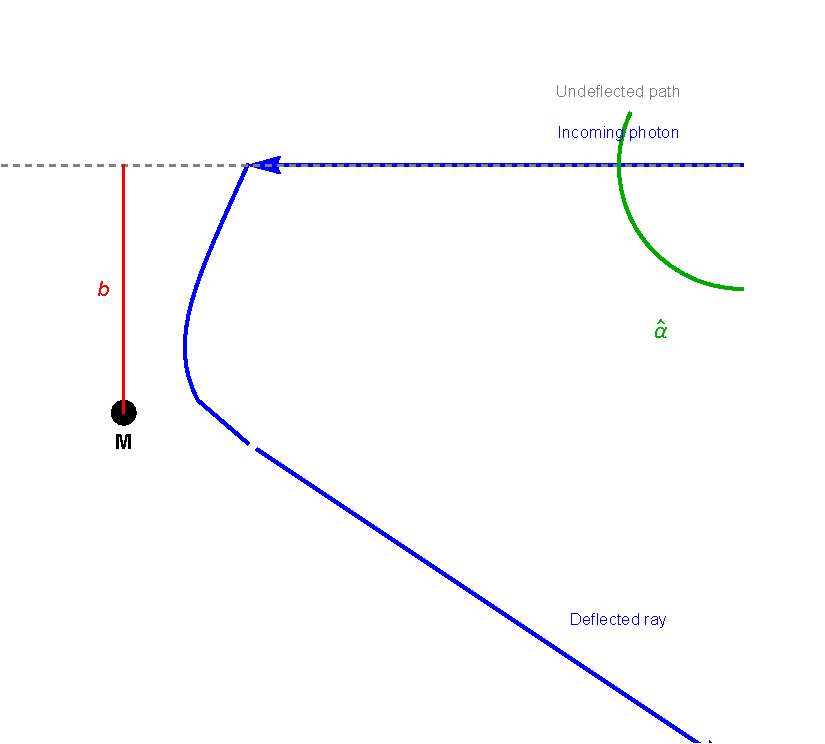
\includegraphics[width=0.75\textwidth]{../Figures/02_Light_Deflection/deflection_geometry.pdf}
    \caption{Geometry of gravitational light deflection by a point mass~$M$.
    A photon approaches from the right with impact parameter~$b$, reaches
    closest approach at~$r_0 \approx b$, and is deflected by
    $\alphahat = 4\Gnewton M/(\speedoflight^2 b)$.  The dashed line shows
    the undeflected path.  Generated by
    \texttt{deflection\_angle.wl}.}
    \label{fig:deflection_geometry}
\end{figure}

\begin{exercise}
\label{ex:gr_vs_newton}
Show that the GR deflection angle~\eqref{eq:alphahat_result} is exactly
twice the Newtonian prediction~\eqref{eq:soldner_deflection}.  Explain
physically why:
\begin{enumerate}[label=(\alph*)]
    \item The Newtonian calculation accounts for the deflection due to the
          gravitational potential (temporal curvature of the metric,
          $g_{tt}$), but ignores spatial curvature ($g_{rr}$).
    \item In GR, both $g_{tt}$ and $g_{rr}$ deviate from flat space by
          the same amount (to leading order in $m/r$), so the spatial
          curvature doubles the deflection.
\end{enumerate}
\textit{Hint:} Expand the Schwarzschild line element in isotropic
coordinates and identify the contributions from the time--time and
space--space components of the metric.
\end{exercise}


% =====================================================================
\section{The Shapiro Time Delay}
\label{sec:shapiro_delay}

In addition to deflecting light, a gravitational field \textit{slows it
down} --- or more precisely, causes an excess travel time relative to the
flat-spacetime path.  This effect was predicted by Irwin Shapiro in 1964
and first measured using radar echoes from Mercury and Venus.

Following Congdon \& Keeton Sec.~3.4.2 (eqs.~3.97--3.110), we derive the
time delay for a photon passing near a point mass.

\subsection{Coordinate Travel Time}
\label{sec:coordinate_travel_time}

For a photon on a null geodesic, we can write $dt/dr$ using the
conserved quantities (Congdon \& Keeton eq.~3.97):
\begin{equation}
    \frac{dt}{dr} = \frac{E / \speedoflight^2}{(1 - \RS/r)}
    \left[\frac{E^2}{\speedoflight^2}
    - \frac{L^2}{r^2}\left(1 - \frac{\RS}{r}\right)
    \right]^{-1/2} .
    \label{eq:dt_dr}
\end{equation}
The coordinate time for the photon to travel from closest approach $r_0$ to
a radial distance~$R$ is (Congdon \& Keeton eq.~3.98):
\begin{equation}
    T(R) = \int_{r_0}^{R} \frac{dt}{dr}\, dr \,.
    \label{eq:travel_time}
\end{equation}
In the weak-field limit ($m/r \ll 1$), expanding to first order gives
(Congdon \& Keeton eq.~3.104):
\begin{equation}
    T(R) \approx \frac{1}{\speedoflight}\sqrt{R^2 - r_0^2}
    + \frac{2m}{\speedoflight}\ln\!\left(
    \frac{R + \sqrt{R^2 - r_0^2}}{r_0}\right)
    + \frac{m}{\speedoflight}\sqrt{\frac{R - r_0}{R + r_0}} \,.
    \label{eq:travel_time_expanded}
\end{equation}

\subsection{The Two Components of Time Delay}
\label{sec:delay_components}

The total time delay $\Delta T$ for a lensed photon (relative to the
unlensed path) has two contributions
(Congdon \& Keeton eqs.~3.107--3.110):
\begin{equation}
    \boxed{
    \Delta T = \underbrace{\frac{\Dd \Ds}{2\speedoflight\,\Dds}
    (\theta - \beta)^2}_{\text{geometric delay}}
    - \underbrace{\frac{4\Gnewton M}{\speedoflight^3}
    \ln|\theta|}_{\text{Shapiro (gravitational) delay}}
    }
    \label{eq:time_delay_total}
\end{equation}
where $\Dd$, $\Ds$, $\Dds$ are the angular diameter distances from
observer to lens, observer to source, and lens to source respectively;
$\theta$ is the image position and $\beta$ the (unlensed) source position.

\begin{remark}
\textbf{Geometric delay:} The lensed ray follows a longer path through
space than the direct (unlensed) ray.  This is a purely geometric effect
and is always positive.

\textbf{Shapiro (gravitational) delay:}  The gravitational potential
slows the effective speed of light near the lens.  Clocks near a mass run
slower (gravitational redshift), so the signal takes longer to traverse the
gravitational potential well.
\end{remark}

\begin{remark}
The total time delay~\eqref{eq:time_delay_total} is closely related to the
\textbf{Fermat potential}, which we will study in detail in Module~6.  The
Fermat potential $\tau(\vectheta)$ encodes both the geometric and
gravitational delays, and its gradient gives the lens equation.  Images
form at stationary points of the Fermat potential (Fermat's principle
applied to gravitational lensing).
\end{remark}

\begin{exercise}
\label{ex:shapiro_sun}
Derive the Shapiro time delay for a radar signal passing near the Sun and
bouncing off a planet at distance~$R$ from the Sun.
\begin{enumerate}[label=(\alph*)]
    \item Show that the excess round-trip travel time is approximately
          \begin{equation*}
              \Delta T \approx \frac{4\Gnewton \Msun}{\speedoflight^3}
              \ln\!\left(\frac{4 R_\oplus R}{r_0^2}\right)
          \end{equation*}
          where $R_\oplus$ is the Earth--Sun distance and $r_0$ the
          closest approach distance.
    \item For a signal grazing the Sun ($r_0 = \Rsun$) bouncing off
          Mercury at inferior conjunction, compute $\Delta T$ numerically.
          You should find $\Delta T \approx 240~\mu\mathrm{s}$.
\end{enumerate}
\end{exercise}


% =====================================================================
\section{Deflection by the Sun}
\label{sec:deflection_sun}

The first and most famous test of the GR deflection formula was
\textbf{Eddington's 1919 solar eclipse expedition}.  During a total
eclipse, stars near the Sun become visible, and their apparent positions
are shifted outward by the gravitational deflection.

For light grazing the limb of the Sun ($b = \Rsun$):
\begin{equation}
    \alphahat_\odot = \frac{4\Gnewton \Msun}{\speedoflight^2\, \Rsun}
    = \frac{4 \times 6.674 \times 10^{-11} \times 1.989 \times 10^{30}}
          {(2.998 \times 10^{8})^2 \times 6.957 \times 10^{8}}
    \approx 8.49 \times 10^{-6}~\text{rad} \,.
    \label{eq:deflection_sun}
\end{equation}
Converting to arcseconds:
\begin{equation}
    \boxed{
    \alphahat_\odot = 1.75''
    }
    \label{eq:deflection_sun_arcsec}
\end{equation}
This is the Newtonian value $0.87''$ \textit{doubled} by general relativity.
Eddington's measurements confirmed the GR prediction (within the
substantial error bars of the time), making Einstein a global celebrity.

\begin{example}
\textbf{Deflection by Jupiter.}  Jupiter has $M_J = 1.898 \times 10^{27}$~kg
and $R_J = 7.149 \times 10^{7}$~m.  The deflection for light grazing
Jupiter's limb is:
\begin{equation}
    \alphahat_J = \frac{4\Gnewton M_J}{\speedoflight^2\, R_J}
    \approx 0.017'' = 17~\text{mas} \,.
    \label{eq:deflection_jupiter}
\end{equation}
This is small but measurable with modern astrometry (e.g., the Gaia
satellite, which achieves $\sim 10~\mu$as precision).
\end{example}

\begin{figure}[ht]
    \centering
    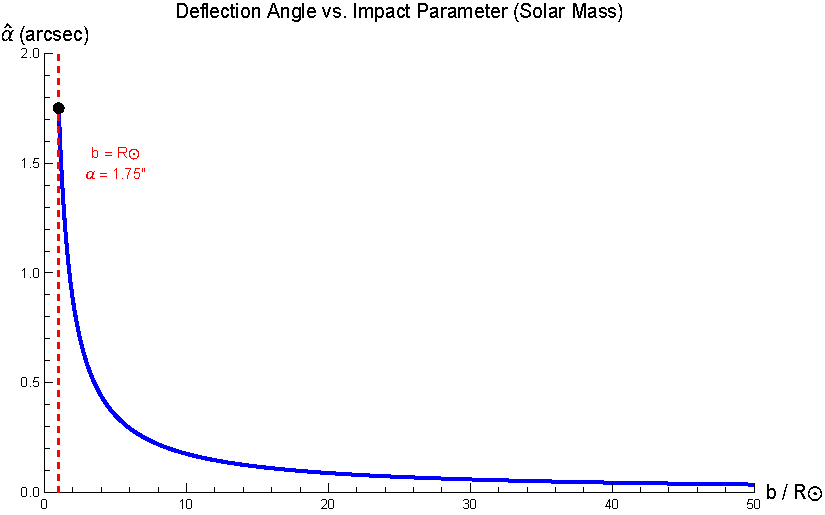
\includegraphics[width=0.75\textwidth]{../Figures/02_Light_Deflection/deflection_vs_impact.pdf}
    \caption{Deflection angle $\alphahat$ as a function of impact
    parameter~$b$ for a solar-mass lens, shown in arcseconds.  The
    deflection falls as $1/b$.  The vertical dashed line marks the solar
    radius ($b = \Rsun$) where $\alphahat = 1.75''$.  Generated by
    \texttt{deflection\_angle.wl}.}
    \label{fig:deflection_vs_impact}
\end{figure}

\begin{exercise}
\label{ex:numerical_deflections}
Compute the deflection angle for light grazing the surface of:
\begin{enumerate}[label=(\alph*)]
    \item The Sun ($M = 1.989 \times 10^{30}$~kg,
          $R = 6.957 \times 10^{8}$~m): verify $\alphahat = 1.75''$.
    \item Jupiter ($M = 1.898 \times 10^{27}$~kg,
          $R = 7.149 \times 10^{7}$~m).
    \item A $10^{12}\,\Msun$ galaxy with effective radius
          $R_e = 10$~kpc, using $b = R_e$.
          Express the result in arcseconds.
\end{enumerate}
\end{exercise}


% =====================================================================
\section{Deflection by Galaxies}
\label{sec:deflection_galaxies}

The astrophysical power of gravitational lensing comes from the fact that
the deflection angles produced by \textit{galaxies} are of order
arcseconds --- large enough to produce multiple images, arcs, and rings
that are observable with ground-based and space-based telescopes.

For a galaxy of mass $M = 10^{12}\,\Msun$ with a typical scale of
$b \sim 10$~kpc~$\approx 3.09 \times 10^{20}$~m:
\begin{equation}
    \alphahat \sim \frac{4\Gnewton M}{\speedoflight^2\, b}
    = \frac{4 \times 6.674 \times 10^{-11} \times 10^{12} \times 1.989 \times 10^{30}}
          {(2.998 \times 10^{8})^2 \times 3.09 \times 10^{20}}
    \approx 3.9''
    \label{eq:deflection_galaxy}
\end{equation}
The corresponding Einstein radius (which we will derive properly in
Module~4) is of order $\sim 1''$, depending on the distance configuration.

\begin{remark}
The Einstein radius $\thetaE$ for a point mass lens at cosmological
distances is:
\begin{equation}
    \thetaE = \sqrt{\frac{4\Gnewton M}{\speedoflight^2}
    \frac{\Dds}{\Dd\,\Ds}} \,.
    \label{eq:einstein_radius_deflection}
\end{equation}
For a $10^{12}\,\Msun$ galaxy at $z_d \sim 0.3$ with a source at
$z_s \sim 1$, this gives $\thetaE \sim 1''$.  Multiple images form
whenever the source lies within $\sim \thetaE$ of the optical axis ---
this is the regime of \textbf{strong gravitational lensing}.  We will
develop this quantitatively in Modules~4--5.
\end{remark}


% =====================================================================
\section{Exact vs.\ Weak-Field Deflection}
\label{sec:exact_vs_approx}

The weak-field formula $\alphahat = 4m/b$ is a first-order approximation
valid when $b \gg \RS$.  For photons passing closer to the mass, higher-order
corrections become important.  The \textit{exact} deflection angle is
obtained by evaluating the integral~\eqref{eq:delta_phi_u2} numerically
(or using elliptic integrals), without the weak-field expansion.

\begin{figure}[ht]
    \centering
    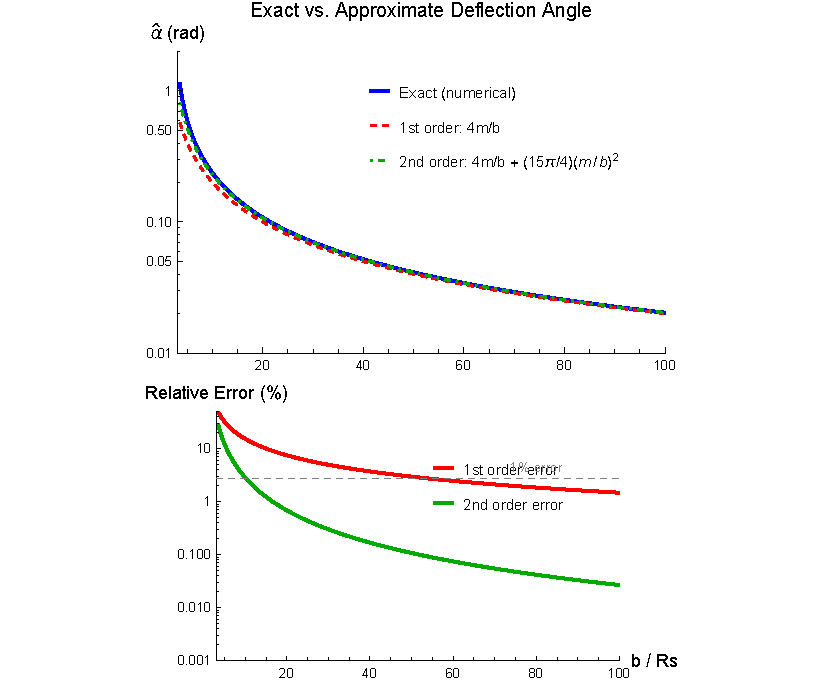
\includegraphics[width=0.75\textwidth]{../Figures/02_Light_Deflection/exact_vs_approx.pdf}
    \caption{Comparison of the exact deflection angle (solid blue, from
    numerical integration) and the weak-field approximations
    $\alphahat = 4m/b$ (dashed red, first order) and including the
    second-order correction (dot-dashed green), as a function of $b/\RS$.
    The lower panel shows the relative error.  The first-order
    approximation has $\sim 15\%$ error at $b = 10\,\RS$ and reaches
    $1\%$ accuracy only for $b \gtrsim 150\,\RS$.  At the photon sphere
    $b = 3\sqrt{3}\,\RS/2$, the exact deflection diverges (the photon
    orbits the mass).  Generated by \texttt{deflection\_angle.wl}.}
    \label{fig:exact_vs_approx}
\end{figure}

The second-order correction has been computed by several authors; the
result is (see, e.g., Keeton \& Petters 2006):
\begin{equation}
    \alphahat = \frac{4m}{b} + \frac{15\pi}{4}\left(\frac{m}{b}\right)^2
    + \order{m/b}^3 \,.
    \label{eq:deflection_second_order}
\end{equation}
The critical impact parameter below which the photon is captured (i.e.,
spirals into the mass) is $b_{\mathrm{crit}} = 3\sqrt{3}\,m =
3\sqrt{3}\,\RS/2$.  This corresponds to the photon sphere derived in
Module~1d.

\begin{exercise}
\label{ex:exact_vs_approx}
For a photon passing a Schwarzschild black hole at impact parameter
$b = 10\,\RS$:
\begin{enumerate}[label=(\alph*)]
    \item Evaluate the deflection integral~\eqref{eq:delta_phi_u2}
          numerically to obtain the exact deflection angle.
    \item Compare with the weak-field approximation
          $\alphahat = 4m/b = 0.2$~rad.  What is the relative error?
    \item Repeat for several values of $b/\RS$ from $5$ to $100$.  At what
          $b/\RS$ does the weak-field approximation first achieve 1\%
          accuracy?
\end{enumerate}
\textit{Use the Mathematica script}
\mathlink{02_Light_Deflection/deflection_angle.wl}{deflection\_angle.wl}
\textit{to verify your results.}
\end{exercise}


% =====================================================================
\section{Summary}
\label{sec:deflection_summary}

\begin{itemize}
    \item Light follows null geodesics in Schwarzschild spacetime.  The
          orbit equation~\eqref{eq:photon_orbit_eq} reduces to an integral
          for the total azimuthal angle change~$\Delta\phi$.

    \item \textbf{Newtonian prediction} (Soldner, 1801):
          $\alphahat_{\mathrm{Newton}} = 2\Gnewton M /
          (\speedoflight^2 b)$.  This accounts for only the
          \textit{temporal} curvature of spacetime.

    \item \textbf{GR prediction} (Einstein, 1915):
          $\alphahat = 4\Gnewton M / (\speedoflight^2 b)$.
          The factor of~$2$ enhancement comes from \textit{spatial}
          curvature, which contributes equally to the deflection.

    \item \textbf{Shapiro time delay:} A gravitational field causes an
          excess travel time $\Delta T$ with geometric and gravitational
          components.  This is connected to the Fermat potential
          (Module~6).

    \item \textbf{Solar deflection:} $\alphahat_\odot = 1.75''$, confirmed
          by Eddington (1919) and modern measurements to $< 0.01\%$.

    \item \textbf{Galaxy-scale lensing:} $\alphahat \sim 1''$--$4''$
          for $\sim 10^{12}\,\Msun$ galaxies at $b \sim 10$~kpc,
          producing multiple images, arcs, and Einstein rings in strong
          lensing.

    \item The weak-field approximation $\alphahat = 4m/b$ converges
          slowly; the error is $\sim 15\%$ at $b = 10\,\RS$ and drops
          below $1\%$ only for $b \gtrsim 150\,\RS$.  The exact
          deflection diverges at the photon sphere ($b_{\mathrm{crit}} =
          3\sqrt{3}\,\RS/2$).
\end{itemize}


% =====================================================================
\section{Problems}
\label{sec:deflection_problems}

\begin{exercise}
\label{ex:soldner_full}
\textbf{(Soldner's Newtonian deflection.)}
Derive the Newtonian deflection angle for a ``corpuscle of light''
traveling at speed $\speedoflight$ past a mass $M$ at impact parameter $b$.
\begin{enumerate}[label=(\alph*)]
    \item Write the Newtonian orbit equation and identify the semi-latus
          rectum $p$ and eccentricity $e$ in terms of $b$, $M$, $\Gnewton$,
          and $\speedoflight$.
    \item Show that the deflection angle is
          $\alphahat_{\mathrm{Newton}} = 2\Gnewton M /
          (\speedoflight^2 b)$ in the weak-field limit.
    \item Compute the Newtonian prediction for the solar deflection.  You
          should get $0.875''$.
\end{enumerate}
\end{exercise}

\begin{exercise}
\label{ex:factor_of_two}
\textbf{(The factor of 2: GR vs.\ Newton.)}
\begin{enumerate}[label=(\alph*)]
    \item Starting from the result $\Delta\phi = \pi + 4m/r_0$, show that
          the GR deflection angle is $\alphahat = 4\Gnewton M /
          (\speedoflight^2 b)$.
    \item The Newtonian result uses only $g_{tt} \approx -(1 - 2\Phi/
          \speedoflight^2)$ where $\Phi = -\Gnewton M/r$.  In GR, the
          spatial part of the Schwarzschild metric also curves:
          $g_{rr} \approx 1 + 2\Gnewton M/(\speedoflight^2 r)$.
          Argue qualitatively (or using the isotropic form of the metric)
          that the spatial curvature contributes an \textit{equal} amount
          of deflection, doubling the Newtonian result.
\end{enumerate}
\end{exercise}

\begin{exercise}
\label{ex:deflections_numerical}
\textbf{(Deflection for Sun, Jupiter, and galaxy.)}
Compute $\alphahat$ for:
\begin{enumerate}[label=(\alph*)]
    \item Light grazing the Sun: $M = 1.989 \times 10^{30}$~kg,
          $b = \Rsun = 6.957 \times 10^{8}$~m.
    \item Light grazing Jupiter: $M = 1.898 \times 10^{27}$~kg,
          $b = R_J = 7.149 \times 10^{7}$~m.
    \item A $10^{12}\,\Msun$ galaxy at $b = 10$~kpc.
\end{enumerate}
Express all answers in arcseconds.  Verify with
\solnlink{02_Light_Deflection/problems\_02.wl}{problems\_02.wl}.
\end{exercise}

\begin{exercise}
\label{ex:shapiro_radar}
\textbf{(Shapiro time delay for radar echoes.)}
A radar signal is sent from Earth, passes near the Sun at closest approach
$r_0$, bounces off Mercury, and returns.
\begin{enumerate}[label=(\alph*)]
    \item Using eq.~\eqref{eq:travel_time_expanded}, show that the excess
          round-trip time is
          \begin{equation*}
              \Delta T \approx
              \frac{4\Gnewton \Msun}{\speedoflight^3}
              \left[\ln\!\left(\frac{4\, R_\oplus\, R_{\mathrm{Merc}}}{r_0^2}
              \right) + 1\right]
          \end{equation*}
          where $R_\oplus = 1.496 \times 10^{11}$~m and
          $R_{\mathrm{Merc}} = 5.79 \times 10^{10}$~m are the
          Earth--Sun and Mercury--Sun distances.
    \item For $r_0 = \Rsun$, compute $\Delta T$ in microseconds.
    \item Shapiro's 1964 measurement using the Haystack radar gave
          $\Delta T = 200 \pm 20~\mu$s.  Is this consistent?
\end{enumerate}
\end{exercise}

\begin{exercise}
\label{ex:strong_field}
\textbf{(Exact vs.\ weak-field deflection.)}
For a photon passing a Schwarzschild mass at impact parameter $b = 10\,\RS$:
\begin{enumerate}[label=(\alph*)]
    \item Evaluate the exact deflection angle by numerically integrating
          eq.~\eqref{eq:delta_phi_u2}.
    \item Compare with the first-order approximation
          $\alphahat_1 = 4m/b$ and the second-order approximation
          $\alphahat_2 = 4m/b + (15\pi/4)(m/b)^2$.
    \item Tabulate the relative error of $\alphahat_1$ and $\alphahat_2$
          for $b/\RS = 5, 10, 20, 50, 100$.
    \item At what value of $b/\RS$ does the first-order approximation
          first achieve $1\%$ accuracy?
\end{enumerate}
\textit{Use}
\mathlink{02_Light_Deflection/deflection_angle.wl}{deflection\_angle.wl}
\textit{to generate and verify your results.}
\end{exercise}

% =============================================================================
% Module 3: Cosmological Distances
% =============================================================================
% Sources: Congdon & Keeton Ch. 3.5, Carroll, Narayan & Bartelmann
% Mathematica: ../Mathematica/03_Cosmological_Distances/
% =============================================================================

\chapter{Cosmological Distances}
\label{ch:cosmological_distances}

% TODO: Module content to be written
% Topics:
% - FRW metric and expanding universe
% - Comoving and proper distances
% - Angular diameter distance
% - Luminosity distance
% - Distance ratios in lensing geometry

% =============================================================================
% Module 4: The Gravitational Lens Equation
% =============================================================================
% Sources: Narayan & Bartelmann Sec. 2.1.3-2.1.5, Congdon & Keeton Ch. 2,
%          Saha et al. Sec. 1
% Mathematica: ../Mathematica/04_Lens_Equation/
% =============================================================================

\chapter{The Gravitational Lens Equation}
\label{ch:lens_equation}

% TODO: Module content to be written
% Topics:
% - Thin lens approximation
% - Source, lens, and image planes
% - Deflection angle and lens equation derivation
% - Reduced deflection angle
% - Multiple images and image multiplicity

% =============================================================================
% Module 5: Magnification, Convergence, and Shear
% =============================================================================
% Sources: Narayan & Bartelmann Sec. 3.2, Congdon & Keeton Ch. 2.6 & 4,
%          Saha et al.
% Mathematica: ../Mathematica/05_Magnification_Convergence_Shear/
% =============================================================================

\chapter{Magnification, Convergence, and Shear}
\label{ch:magnification_convergence_shear}

% TODO: Module content to be written
% Topics:
% - Jacobian of the lens mapping
% - Convergence (kappa) and surface mass density
% - Shear (gamma) components
% - Magnification tensor and magnification factor
% - Critical curves and caustics introduction

% =============================================================================
% Module 6: Fermat's Principle and Time Delays
% =============================================================================
% Sources: Saha et al. Sec. 1.2-1.3, Narayan & Bartelmann Sec. 3.3,
%          Congdon & Keeton Ch. 4.3-4.4
% Mathematica: ../Mathematica/06_Fermat_Time_Delays/
% =============================================================================

\chapter{Fermat's Principle and Time Delays}
\label{ch:fermat_time_delays}

\begin{quote}
\textit{The positions of the images of a gravitational lens are determined
by Fermat's principle: images form at stationary points of the arrival
time.  The time delays between multiple images, in turn, give us a
direct measurement of cosmological distances --- and hence the Hubble
constant.}
\hfill --- Narayan \& Bartelmann (1997)
\end{quote}

\noindent
In Module~\ref{ch:lens_equation} we derived the lens equation
$\vecbeta = \vectheta - \vecalpha(\vectheta)$ as a geometric
consequence of light deflection.  In Module~\ref{ch:light_deflection}
we computed the Shapiro time delay experienced by photons passing
through a gravitational potential, and in
Module~\ref{ch:linearized_gravity} we introduced the effective
refractive index of a weak gravitational field.

In this module we show that the lens equation itself emerges from a
variational principle: images form at stationary points of the
\textbf{arrival-time surface}.  This elegant reformulation ---
Fermat's principle for gravitational lensing --- not only provides a
deeper understanding of image formation, but also yields
\textbf{observable time delays} between multiple images.  These time
delays are directly proportional to $\Hubble^{-1}$, making
multiply-imaged variable sources (such as quasars) a powerful and
independent probe of the Hubble constant.

\medskip
\noindent
\textbf{Companion Mathematica files:}
\begin{itemize}[nosep]
    \item \mathlink{06_Fermat_Time_Delays/time_delay_function.wl}{time\_delay\_function.wl}
          --- symbolic computation of the Fermat potential, verification
          that $\nabla\tau = 0$ recovers the lens equation, time delay
          formulas for point mass and SIS lenses, numerical $\Hubble$
          estimation, and publication-quality figure generation
    \item \mathlink{06_Fermat_Time_Delays/arrival_time_surface.nb}{arrival\_time\_surface.nb}
          --- interactive notebook: 3D arrival-time surface with slider
          for source position, contour plots with critical curves,
          time delay visualization
\end{itemize}


% =====================================================================
\section{Introduction: From Geometry to a Variational Principle}
\label{sec:fermat_intro}

The lens equation $\vecbeta = \vectheta - \vecalpha(\vectheta)$ was
derived in Module~\ref{ch:lens_equation} by tracing light rays through
the lensing geometry.  While this approach is direct and intuitive, it
does not explain \textit{why} light ``chooses'' particular paths through
the lens plane, nor does it immediately reveal the relative arrival times
of multiple images.

A deeper perspective comes from \textbf{Fermat's principle}: among all
possible paths from source to observer, light follows those for which the
travel time is \textit{stationary} (a minimum, maximum, or saddle point
of the arrival time).  In classical optics, Fermat's principle explains
Snell's law and the focusing properties of lenses.  In gravitational
lensing, it does far more:
\begin{enumerate}
    \item It \textbf{derives} the lens equation as the stationarity
          condition $\nabla_{\vectheta}\, t = 0$.
    \item It \textbf{classifies} multiple images by the nature of the
          stationary point (minimum, saddle, or maximum), which
          determines their parity and arrival order.
    \item It produces \textbf{observable time delays} between multiple
          images, which can be used to measure the Hubble constant.
\end{enumerate}

The key quantity is the \textbf{time delay function} (or
\textbf{arrival-time surface}) $t(\vectheta)$, which gives the arrival
time of a photon traveling from a source at $\vecbeta$ via the lens
plane at $\vectheta$ to the observer.  Images form at the stationary
points of $t(\vectheta)$, and the differences in $t$ between stationary
points give the time delays.


% =====================================================================
\section{The Time Delay Function}
\label{sec:time_delay_function}

Consider a photon emitted by a source at angular position $\vecbeta$ in
the source plane.  The photon passes through the lens plane at angular
position $\vectheta$ and arrives at the observer.  The total travel time
relative to the unperturbed (unlensed, straight-line) path consists of
two contributions:

\begin{itemize}
    \item \textbf{Geometric delay} (extra path length): The deflected ray
          travels a longer geometric path than the straight-line ray.  In
          the small-angle, thin-lens approximation, the extra path length
          corresponds to an angular excess of $\half|\vectheta - \vecbeta|^2$
          (see Module~\ref{ch:lens_equation}, Section~\ref{sec:lensing_geometry}).
    \item \textbf{Shapiro (gravitational) delay}: The photon passes
          through the gravitational potential of the lens, experiencing the
          time delay derived in Module~\ref{ch:light_deflection}.  In the
          thin-lens formalism, this delay is encoded in the
          \textbf{lensing potential} $\psiL(\vectheta)$
          (Module~\ref{ch:magnification_convergence_shear}).
\end{itemize}

Combining these contributions, the total arrival time is
(Narayan \& Bartelmann eq.~21; Congdon \& Keeton eq.~4.46):
\begin{equation}
    \boxed{
    t(\vectheta) = \frac{(1 + z_d)}{\speedoflight}\,
    \frac{\Dd\,\Ds}{\Dds}\,
    \left[\half|\vectheta - \vecbeta|^2 - \psiL(\vectheta)\right]
    + \text{const}
    }
    \label{eq:time_delay_function}
\end{equation}
where $z_d$ is the redshift of the lens, the angular diameter distances
$\Dd$, $\Ds$, $\Dds$ are defined in Module~\ref{ch:cosmological_distances},
and the constant is an irrelevant additive term that depends on the
unperturbed travel time.

The factor $(1 + z_d)$ converts from the lens-frame time to the
observer-frame time (cosmological time dilation).  The combination
$\Dd\,\Ds / \Dds$ is the \textbf{effective lensing distance}, which
encodes the geometry of the observer--lens--source system.

\begin{definition}[Fermat potential]
The dimensionless quantity
\begin{equation}
    \boxed{
    \tau(\vectheta, \vecbeta) = \half|\vectheta - \vecbeta|^2
    - \psiL(\vectheta)
    }
    \label{eq:fermat_potential}
\end{equation}
is called the \textbf{Fermat potential} (or \textbf{time delay
potential}).  The arrival time is proportional to $\tau$:
\begin{equation}
    t(\vectheta) = \frac{(1 + z_d)}{\speedoflight}\,
    \frac{\Dd\,\Ds}{\Dds}\, \tau(\vectheta, \vecbeta)
    + \text{const} \,.
    \label{eq:t_tau_relation}
\end{equation}
\end{definition}

\begin{remark}
The Fermat potential has a simple physical interpretation:
\begin{itemize}[nosep]
    \item The first term $\half|\vectheta - \vecbeta|^2$ is the
          \textbf{geometric delay}: it penalizes paths where the ray in the
          lens plane ($\vectheta$) is far from the straight-line direction
          ($\vecbeta$).
    \item The second term $-\psiL(\vectheta)$ is the
          \textbf{gravitational (Shapiro) delay}: the lensing potential
          $\psiL > 0$ in the vicinity of the lens, so this term
          \textit{reduces} the arrival time --- photons passing through a
          deeper potential arrive earlier due to the Shapiro effect
          (recall Module~\ref{ch:light_deflection}).
\end{itemize}
The competition between geometric and gravitational delay determines the
structure of the arrival-time surface and hence the number and types of
images.
\end{remark}


% =====================================================================
\section{Fermat's Principle and the Lens Equation}
\label{sec:fermat_principle}

\textbf{Fermat's principle} states that images form at stationary points
of the arrival time $t(\vectheta)$, or equivalently, at stationary points
of the Fermat potential $\tau(\vectheta, \vecbeta)$:
\begin{equation}
    \nabla_{\vectheta}\, t(\vectheta) = 0
    \quad \Longleftrightarrow \quad
    \nabla_{\vectheta}\, \tau(\vectheta, \vecbeta) = 0 \,.
    \label{eq:fermat_condition}
\end{equation}

Computing the gradient of $\tau$:
\begin{align}
    \nabla_{\vectheta}\, \tau &= \nabla_{\vectheta}\left[
    \half|\vectheta - \vecbeta|^2 - \psiL(\vectheta)\right]
    \nonumber \\
    &= (\vectheta - \vecbeta) - \nabla\psiL(\vectheta) \,.
    \label{eq:grad_tau}
\end{align}
Setting this to zero:
\begin{equation}
    \vectheta - \vecbeta - \nabla\psiL(\vectheta) = 0
    \qquad \Longrightarrow \qquad
    \vecbeta = \vectheta - \nabla\psiL(\vectheta) \,.
    \label{eq:lens_eq_from_fermat}
\end{equation}
Since the reduced deflection angle is $\vecalpha(\vectheta) = \nabla\psiL(\vectheta)$
(from Module~\ref{ch:magnification_convergence_shear}), this is precisely
the \textbf{lens equation}:
\begin{equation}
    \boxed{
    \vecbeta = \vectheta - \vecalpha(\vectheta)
    }
    \label{eq:lens_eq_fermat}
\end{equation}

\begin{remark}
This is a remarkable result: the lens equation, which we previously derived
from ray-tracing geometry, follows directly from the
\textbf{stationarity of the arrival time}.  Fermat's principle provides
a variational derivation of the fundamental equation of gravitational
lensing.  The connection between the gradient of the lensing potential and
the deflection angle, $\vecalpha = \nabla\psiL$, was established in
Module~\ref{ch:magnification_convergence_shear} from the Poisson equation
$\nabla^2\psiL = 2\kappab$.
\end{remark}


% =====================================================================
\section{Classification of Images: Morse Theory}
\label{sec:morse_theory}

At each stationary point $\vectheta_i$ of the Fermat potential (i.e.,
at each image position), we can characterize the nature of the
stationary point by the \textbf{Hessian matrix} of $\tau$:
\begin{equation}
    T_{ab} = \frac{\partial^2 \tau}{\partial\theta_a\,\partial\theta_b}
    = \delta_{ab} - \frac{\partial^2\psiL}{\partial\theta_a\,\partial\theta_b}
    = \Amat_{ab} \,,
    \label{eq:hessian_tau}
\end{equation}
where $\Amat_{ab}$ is the \textbf{Jacobian matrix} of the lens mapping
(the inverse magnification matrix, from
Module~\ref{ch:magnification_convergence_shear}).

The eigenvalues of $T_{ab}$ at a stationary point determine the
\textit{type} of the image.  There are exactly three possibilities,
classified by \textbf{Morse theory}:

\begin{enumerate}
    \item \textbf{Type I image --- Minimum of $\tau$:}
    Both eigenvalues of $T$ are positive.  Equivalently,
    $\det(\Amat) > 0$ and $\mathrm{tr}(\Amat) > 0$.  The magnification
    $\mu = 1/\det(\Amat) > 0$ (positive parity: the image is not
    mirror-reflected).  This image corresponds to the \textit{minimum}
    of the arrival-time surface and therefore \textbf{arrives first}.

    \item \textbf{Type II image --- Saddle point of $\tau$:}
    One eigenvalue is positive and one is negative.  Equivalently,
    $\det(\Amat) < 0$.  The magnification $\mu = 1/\det(\Amat) < 0$
    (negative parity: the image is mirror-reflected).

    \item \textbf{Type III image --- Maximum of $\tau$:}
    Both eigenvalues of $T$ are negative.  Equivalently,
    $\det(\Amat) > 0$ and $\mathrm{tr}(\Amat) < 0$.  The magnification
    $\mu = 1/\det(\Amat) > 0$ (positive parity).  This image
    corresponds to the \textit{maximum} of the arrival-time surface and
    therefore \textbf{arrives last}.
\end{enumerate}

\begin{table}[ht]
\centering
\caption{Classification of images by Morse type.  The Hessian of the
Fermat potential at each image determines its type, parity, and arrival
order.}
\label{tab:morse_types}
\begin{tabular}{lccccc}
\toprule
\textbf{Type} & \textbf{Stationary point} & \textbf{Eigenvalues}
& $\det(\Amat)$ & \textbf{Parity} & \textbf{Arrival} \\
\midrule
I   & Minimum & $+, +$ & $> 0$ & $+$ (same) & First \\
II  & Saddle  & $+, -$ & $< 0$ & $-$ (flipped) & Middle \\
III & Maximum & $-, -$ & $> 0$ & $+$ (same) & Last \\
\bottomrule
\end{tabular}
\end{table}

\begin{theorem}[Burke's Odd-Number Theorem]
\label{thm:odd_number}
For a \textbf{transparent} lens (i.e., a lens with a smooth, bounded
surface mass density $\Sigma(\vectheta)$ that falls off sufficiently
rapidly at large $|\vectheta|$), the total number of images is always
\textbf{odd}.  Specifically, if we denote by $n_{\mathrm{min}}$,
$n_{\mathrm{sad}}$, and $n_{\mathrm{max}}$ the numbers of minima,
saddle points, and maxima of $\tau$, then:
\begin{equation}
    n_{\mathrm{min}} - n_{\mathrm{sad}} + n_{\mathrm{max}} = 1 \,.
    \label{eq:odd_number}
\end{equation}
This is a topological result from Morse theory.
\end{theorem}

\begin{remark}
The odd-number theorem explains why a point mass lens produces two
bright images plus one highly demagnified image at the center (which is
a maximum of $\tau$).  In practice, the central image is so faint that
it is unobservable, and we see only the two images $\theta_\pm$ from
Module~\ref{ch:lens_equation}.  For an extended galaxy lens (such as the
SIS model, Module~7), strong lensing typically produces either one image
(when the source is outside the caustic) or three images (when the
source is inside the caustic, with one image usually highly
demagnified).
\end{remark}


% =====================================================================
\section{The Arrival-Time Surface}
\label{sec:arrival_time_surface}

The arrival-time surface is the three-dimensional plot of
$\tau(\vectheta)$ as a function of the two-dimensional image-plane
position $\vectheta = (\theta_1, \theta_2)$ for a fixed source position
$\vecbeta$.  This is the iconic visualization of Fermat's principle in
gravitational lensing.

\subsection{Point Mass Lens}

For a point mass lens with Einstein radius $\thetaE$, the lensing
potential is (from Module~\ref{ch:magnification_convergence_shear}):
\begin{equation}
    \psiL(\vectheta) = \thetaE^2\, \ln|\vectheta| \,.
    \label{eq:psi_point_mass}
\end{equation}
The Fermat potential becomes:
\begin{equation}
    \tau(\vectheta, \vecbeta) = \half|\vectheta - \vecbeta|^2
    - \thetaE^2\, \ln|\vectheta| \,.
    \label{eq:tau_point_mass}
\end{equation}

For a source at $\vecbeta = (\beta, 0)$ with $\beta > 0$ (placing the
source along the $\theta_1$-axis without loss of generality by the
azimuthal symmetry of the lens), the arrival-time surface
$\tau(\theta_1, \theta_2)$ has exactly \textbf{two} stationary points
in the region $|\vectheta| > 0$:
\begin{itemize}
    \item A \textbf{minimum} (Type~I) at $\vectheta = (\theta_+, 0)$,
          where $\theta_+ = (\beta + \sqrt{\beta^2 + 4\thetaE^2})/2$ is
          the primary image from eq.~\eqref{eq:image_positions}.  This
          image arrives \textit{first}.
    \item A \textbf{saddle point} (Type~II) at
          $\vectheta = (\theta_-, 0)$, where
          $\theta_- = (\beta - \sqrt{\beta^2 + 4\thetaE^2})/2$ is the
          secondary image.  This image arrives \textit{second}.
\end{itemize}

In addition, there is a formal maximum at $\vectheta = \mathbf{0}$ (the
lens position), but $\psiL$ diverges logarithmically there, so this
image has zero magnification and is unobservable.

\begin{figure}[ht]
    \centering
    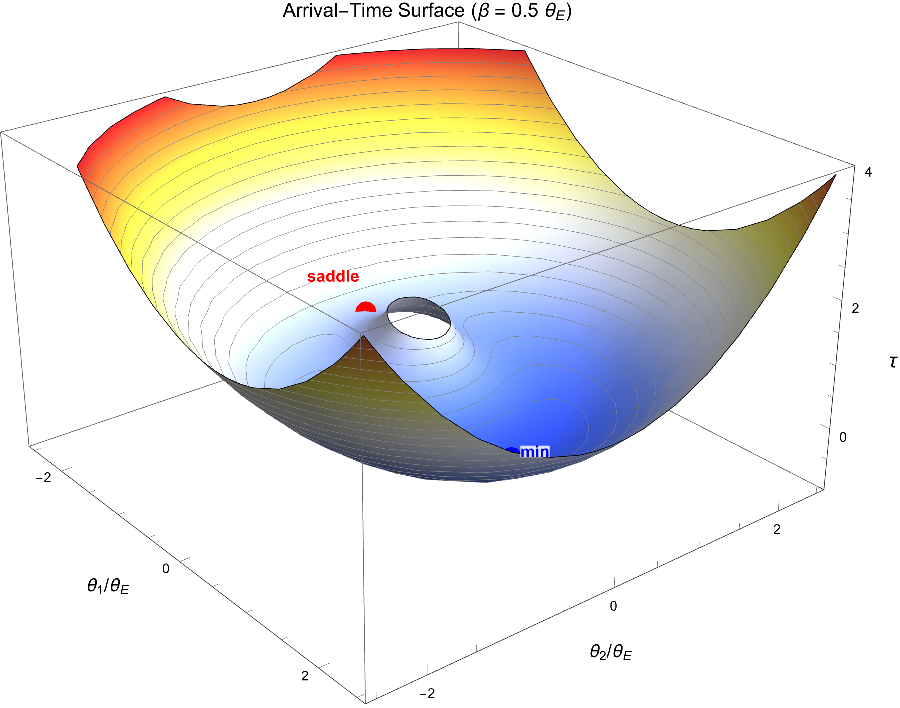
\includegraphics[width=0.85\textwidth]{../Figures/06_Fermat_Time_Delays/arrival_time_surface.pdf}
    \caption{The arrival-time surface $\tau(\theta_1, \theta_2)$ for a
    point mass lens with source at $\vecbeta = (0.5, 0)\,\thetaE$.
    The surface shows a minimum (Type~I image, blue dot) and a saddle
    point (Type~II image, red dot).  The minimum has the smaller
    arrival time and corresponds to the image that is observed first.
    The difference in $\tau$ between the two stationary points gives
    the dimensionless time delay.  Generated by
    \texttt{time\_delay\_function.wl}.}
    \label{fig:arrival_time_surface}
\end{figure}

\subsection{The Einstein Ring as a Degenerate Minimum}

When the source is exactly behind the lens ($\vecbeta = 0$), the
Fermat potential becomes circularly symmetric:
\begin{equation}
    \tau(\vectheta, \mathbf{0}) = \half|\vectheta|^2
    - \thetaE^2\, \ln|\vectheta| \,.
\end{equation}
The stationarity condition $d\tau/d|\vectheta| = 0$ gives
$|\vectheta| = \thetaE$, which is the Einstein ring.  The minimum
of $\tau$ is no longer an isolated point but a \textbf{circle} of
stationary points --- the Einstein ring is a degenerate minimum of
the arrival-time surface.

\begin{figure}[ht]
    \centering
    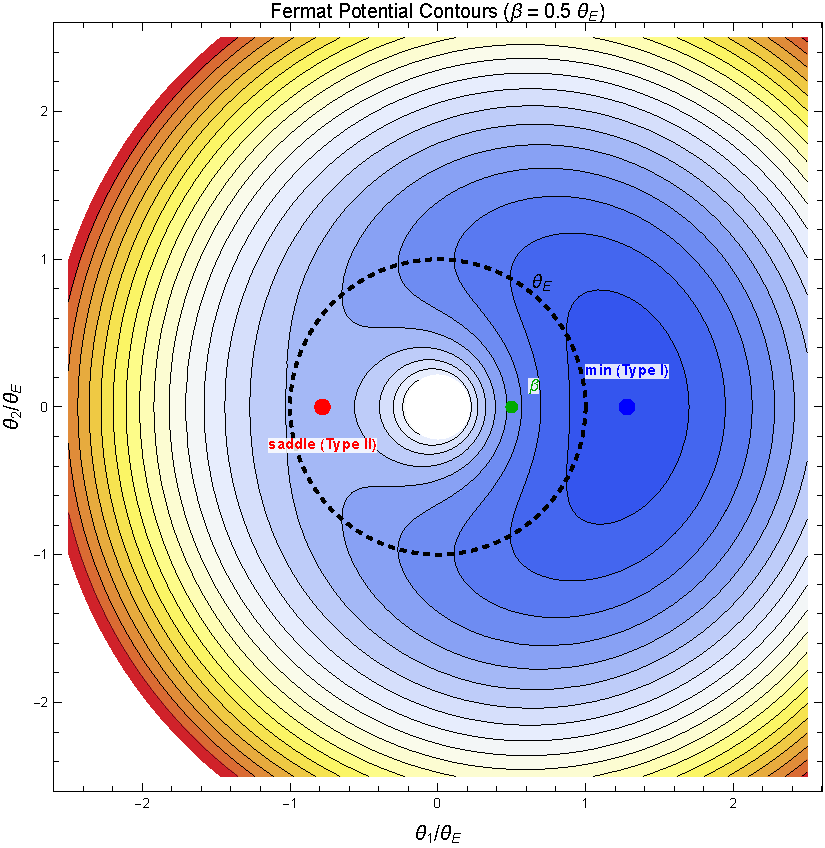
\includegraphics[width=0.78\textwidth]{../Figures/06_Fermat_Time_Delays/arrival_time_contours.pdf}
    \caption{Contour plot of the Fermat potential $\tau(\theta_1,
    \theta_2)$ for a point mass lens with $\vecbeta = (0.5, 0)\,\thetaE$.
    The two stationary points (minimum and saddle) are marked.  The
    critical curve (Einstein ring, dashed circle) is overlaid.
    Generated by \texttt{time\_delay\_function.wl}.}
    \label{fig:arrival_time_contours}
\end{figure}


% =====================================================================
\section{Observable Time Delays}
\label{sec:observable_time_delays}

The arrival time at each image $\vectheta_i$ is given by
eq.~\eqref{eq:time_delay_function}.  The \textbf{time delay} between
two images $i$ and $j$ is the difference in their arrival times:
\begin{equation}
    \boxed{
    \Delta t_{ij} = t(\vectheta_i) - t(\vectheta_j)
    = \frac{(1 + z_d)}{\speedoflight}\,
    \frac{\Dd\,\Ds}{\Dds}\,
    \left[\tau(\vectheta_i, \vecbeta) - \tau(\vectheta_j, \vecbeta)\right]
    }
    \label{eq:time_delay_between_images}
\end{equation}

This quantity is \textbf{directly observable}: if the source is variable
(as quasars are), the light curves measured at the two image positions
will show the same variability pattern, but shifted by $\Delta t_{ij}$.
By cross-correlating the light curves, one can extract $\Delta t_{ij}$
to high precision.

\begin{remark}
The time delay $\Delta t_{ij}$ depends on three ingredients:
\begin{enumerate}[nosep]
    \item The \textbf{cosmological distances} $(1+z_d)\,\Dd\,\Ds/\Dds$,
          which encode the expansion history of the universe.
    \item The \textbf{image positions} $\vectheta_i$, $\vectheta_j$,
          which are directly observed.
    \item The \textbf{lensing potential} $\psiL(\vectheta)$, which must
          be modeled from the observed lens properties (mass distribution,
          image positions, fluxes, etc.).
\end{enumerate}
Given items (2) and (3), a measurement of $\Delta t_{ij}$ constrains
the distance combination in item (1) --- and hence the cosmological
parameters.
\end{remark}


% =====================================================================
\section{Time Delay and the Hubble Constant}
\label{sec:time_delay_H0}

The key cosmological application of time delays is the measurement of
the Hubble constant $\Hubble$.  The distance combination
$\Dd\,\Ds / \Dds$ is an angular diameter distance ratio that scales
inversely with the Hubble constant:
\begin{equation}
    \frac{\Dd\,\Ds}{\Dds} \propto \frac{1}{\Hubble} \,.
    \label{eq:distance_H0_scaling}
\end{equation}
This follows from the definition of angular diameter distances in
Module~\ref{ch:cosmological_distances}: all comoving distances scale as
$\speedoflight / \Hubble$ times a dimensionless integral over the
expansion history.

Therefore, the time delay between images scales as:
\begin{equation}
    \boxed{
    \Delta t \propto \Hubble^{-1}
    }
    \label{eq:Dt_H0}
\end{equation}

This is the basis of \textbf{time-delay cosmography}: by measuring
$\Delta t$ from monitoring campaigns and modeling the lens potential
$\psiL$, one can determine $\Hubble$ \textit{independently of the
cosmic distance ladder}.  The method is sometimes called ``one-step''
distance measurement, because it converts an observed time delay
directly into a physical distance.

\begin{remark}
To extract $\Hubble$ from a time delay measurement, one needs:
\begin{enumerate}[nosep]
    \item A precise measurement of $\Delta t$ (from light curve
          monitoring of a multiply-imaged variable source).
    \item The lens and source redshifts $z_d$, $z_s$.
    \item A model for the lens mass distribution $\psiL(\vectheta)$,
          constrained by the observed image positions, fluxes, and
          extended image structure.
    \item A cosmological model (usually flat $\Lambda$CDM with $\Omegam$
          fixed) to convert the distance ratio into $\Hubble$.
\end{enumerate}
The main systematic uncertainty is the lens model degeneracy (the
``mass-sheet degeneracy''), which we will encounter in later modules.
\end{remark}

\subsection{Observational Milestones}

Time-delay cosmography has been applied to a growing number of
multiply-imaged quasars:
\begin{itemize}
    \item \textbf{Q0957+561} (Walsh, Carswell \& Weymann 1979): the first
          discovered gravitational lens.  The time delay ($\Delta t \approx
          417$~days) was measured after years of photometric monitoring.
    \item \textbf{B1608+656}: a four-image lens system with three
          independent time delays, providing strong constraints.
    \item \textbf{H0LiCOW/TDCOSMO} (2017--present): a systematic program
          combining precise time delays from COSMOGRAIL monitoring with
          detailed lens models and line-of-sight structure analysis.
          Their combined result gives $\Hubble = 73.3^{+1.7}_{-1.8}$~km\,s$^{-1}$\,Mpc$^{-1}$,
          in agreement with local distance ladder measurements and in
          some tension with the CMB value ($\Hubble \approx 67$~km\,s$^{-1}$\,Mpc$^{-1}$
          from Planck).
\end{itemize}


% =====================================================================
\section{Example: Point Mass Time Delay}
\label{sec:point_mass_time_delay}

We now compute the time delay for a point mass lens explicitly.  This
illustrative calculation demonstrates the method and gives a sense of
the physical scales involved.

\subsection{Fermat Potential for the Point Mass}

Using the lensing potential $\psiL(\vectheta) = \thetaE^2 \ln|\vectheta|$
and working in units of $\thetaE$ (i.e., defining $x = \theta/\thetaE$
and $y = \beta/\thetaE$), the Fermat potential along the symmetry axis
(where both images lie for a point mass) is:
\begin{equation}
    \tau(x) = \half(x - y)^2 - \ln|x| \,,
    \label{eq:tau_point_mass_1d}
\end{equation}
where we have set $\thetaE = 1$ in the logarithmic term.

The two image positions are $x_\pm = (y \pm \sqrt{y^2 + 4})/2$.

\subsection{Time Delay Computation}

The Fermat potential at the two images is:
\begin{align}
    \tau(x_+) &= \half(x_+ - y)^2 - \ln x_+ \,, \\
    \tau(x_-) &= \half(x_- - y)^2 - \ln|x_-| \,.
\end{align}
The dimensionless time delay is $\Delta\tau = \tau(x_-) - \tau(x_+)$
(since $\tau(x_-) > \tau(x_+)$, the saddle image arrives later).

After algebraic simplification (verified in
\mathlink{06_Fermat_Time_Delays/time_delay_function.wl}{time\_delay\_function.wl}),
the result is:
\begin{equation}
    \boxed{
    \Delta\tau = \frac{y\sqrt{y^2 + 4}}{2}
    + \ln\!\left(\frac{\sqrt{y^2 + 4} + y}{\sqrt{y^2 + 4} - y}\right)
    }
    \label{eq:delta_tau_point_mass}
\end{equation}
where $y = \beta / \thetaE$ is the dimensionless source position.

The physical time delay is:
\begin{equation}
    \Delta t = \frac{(1 + z_d)}{\speedoflight}\,
    \frac{\Dd\,\Ds}{\Dds}\, \thetaE^2\, \Delta\tau \,.
    \label{eq:delta_t_point_mass}
\end{equation}
Using $\thetaE^2 = 4\Gnewton M / (\speedoflight^2) \cdot \Dds / (\Dd\,\Ds)$:
\begin{equation}
    \Delta t = \frac{4\Gnewton M}{\speedoflight^3}\, (1 + z_d)\, \Delta\tau
    = \frac{\RS}{\speedoflight}\, (1 + z_d)\, \Delta\tau \,,
    \label{eq:delta_t_schwarzschild}
\end{equation}
where $\RS = 2\Gnewton M / \speedoflight^2$ is the Schwarzschild
radius.

\begin{example}
\label{ex:point_mass_numerical}
\textbf{Numerical time delay for a galaxy-mass point lens.}

Consider a lens mass $M = 10^{12}\,\Msun$ at $z_d = 0.3$ with a source
at $\beta = 0.5\,\thetaE$ ($y = 0.5$).  The Schwarzschild radius is:
\begin{equation*}
    \RS = \frac{2 \times 6.674 \times 10^{-11} \times
    10^{12} \times 1.989 \times 10^{30}}{(2.998 \times 10^8)^2}
    \approx 2.95 \times 10^{15}~\text{m}
    \approx 0.096~\text{pc} \,.
\end{equation*}
For $y = 0.5$: $\sqrt{y^2 + 4} = \sqrt{4.25} \approx 2.0616$.
\begin{align*}
    \Delta\tau &= \frac{0.5 \times 2.0616}{2}
    + \ln\!\left(\frac{2.0616 + 0.5}{2.0616 - 0.5}\right) \\
    &= 0.5154 + \ln(1.6401)
    = 0.5154 + 0.4947 = 1.0101 \,.
\end{align*}
The time delay is:
\begin{equation*}
    \Delta t = \frac{2.95 \times 10^{15}}{2.998 \times 10^8}
    \times 1.3 \times 1.0101
    \approx 1.29 \times 10^{7}~\text{s}
    \approx 149~\text{days} \,.
\end{equation*}
This is a realistic order of magnitude --- observed time delays in
galaxy-scale lens systems range from days to months.  Computed and
verified in
\mathlink{06_Fermat_Time_Delays/time_delay_function.wl}{time\_delay\_function.wl}.
\end{example}

\begin{figure}[ht]
    \centering
    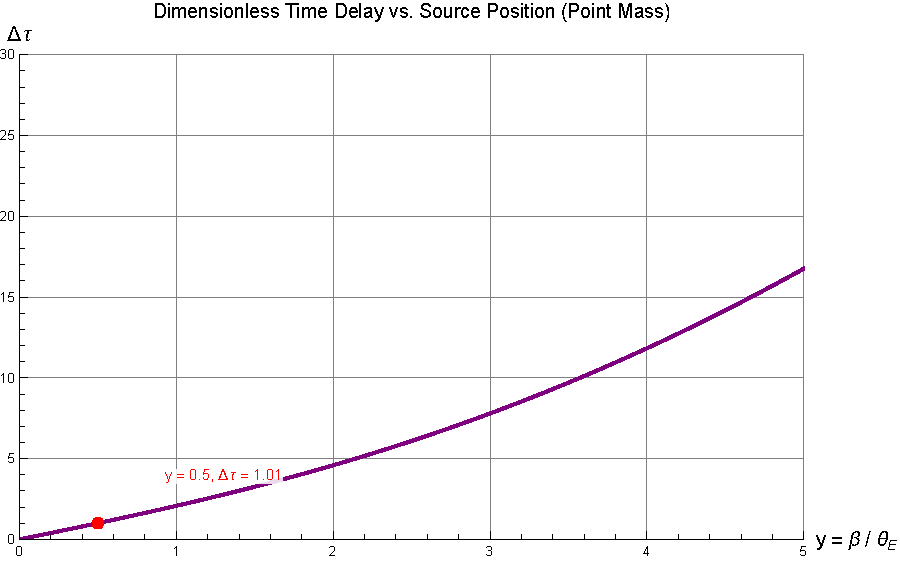
\includegraphics[width=0.78\textwidth]{../Figures/06_Fermat_Time_Delays/time_delay_vs_beta.pdf}
    \caption{Dimensionless time delay $\Delta\tau$ between the two images
    of a point mass lens as a function of the source position
    $y = \beta / \thetaE$.  The time delay increases with the source
    offset.  For $y \to 0$ (Einstein ring limit), $\Delta\tau \to 0$
    because the two images become symmetric.  Generated by
    \texttt{time\_delay\_function.wl}.}
    \label{fig:time_delay_vs_beta}
\end{figure}


% =====================================================================
\section{Example: SIS Time Delay}
\label{sec:sis_time_delay}

As a preview for Module~7 (axially symmetric lens models), we state the
time delay for the \textbf{singular isothermal sphere} (SIS).  The SIS
is characterized by its velocity dispersion $\sigma_v$, and its Einstein
radius is $\thetaE = 4\pi\,(\sigma_v/\speedoflight)^2\,\Dds/\Ds$.

For a source inside the Einstein ring ($\beta < \thetaE$), the SIS
produces two images at positions $\theta_\pm = \beta \pm \thetaE$
(both on the same side of the lens for $\theta_+$, opposite for
$\theta_-$).  The lensing potential is
$\psiL(\vectheta) = \thetaE\,|\vectheta|$, and the time delay between
the two images is:
\begin{equation}
    \boxed{
    \Delta t_{\mathrm{SIS}} = \frac{(1 + z_d)}{\speedoflight}\,
    \frac{\Dd\,\Ds}{\Dds}\,
    \frac{\thetaE^2}{2}\left(
    \frac{\theta_+^2 - \theta_-^2}{\thetaE^2}
    \right)
    = \frac{(1 + z_d)}{2\speedoflight}\,
    \frac{\Dd\,\Ds}{\Dds}\,
    \left(\theta_+^2 - \theta_-^2\right)
    }
    \label{eq:time_delay_SIS}
\end{equation}
Since $\theta_+^2 - \theta_-^2 = (\theta_+ + \theta_-)(\theta_+ - \theta_-)
= 2\beta \cdot 2\thetaE = 4\beta\,\thetaE$, this simplifies to:
\begin{equation}
    \Delta t_{\mathrm{SIS}} = \frac{2(1 + z_d)}{\speedoflight}\,
    \frac{\Dd\,\Ds}{\Dds}\, \beta\,\thetaE \,.
    \label{eq:time_delay_SIS_simple}
\end{equation}
For the SIS, the time delay is proportional to the source position ---
the further the source from the optical axis, the larger the time delay.
This simple relation makes the SIS a useful ``first approximation'' for
time-delay estimates.


% =====================================================================
\section{Summary}
\label{sec:fermat_summary}

\begin{itemize}
    \item The \textbf{time delay function}
          $t(\vectheta) \propto \tau(\vectheta, \vecbeta)$
          gives the arrival time of a photon passing through the lens
          plane at $\vectheta$.  The \textbf{Fermat potential}
          $\tau = \half|\vectheta - \vecbeta|^2 - \psiL(\vectheta)$
          combines the geometric delay (extra path length) and the
          Shapiro delay (gravitational time delay from the lensing
          potential).

    \item \textbf{Fermat's principle}: images form at stationary points
          of $\tau(\vectheta)$.  The condition $\nabla_{\vectheta}\tau = 0$
          recovers the lens equation
          $\vecbeta = \vectheta - \nabla\psiL = \vectheta - \vecalpha$.

    \item Images are classified by \textbf{Morse theory}:
          \textbf{Type~I} (minimum, positive parity, arrives first),
          \textbf{Type~II} (saddle, negative parity),
          \textbf{Type~III} (maximum, positive parity, arrives last).
          \textbf{Burke's theorem}: the number of images is always odd
          for a transparent lens.

    \item The \textbf{arrival-time surface} $\tau(\theta_1, \theta_2)$
          visualizes the image-forming process.  For a point mass lens,
          it has a minimum and a saddle point (plus a singular maximum
          at the lens center).

    \item The \textbf{time delay between images}
          $\Delta t_{ij} \propto (1+z_d)\,\Dd\Ds/\Dds \times
          [\tau(\vectheta_i) - \tau(\vectheta_j)]$
          is directly observable by monitoring variable sources.

    \item $\Delta t \propto \Hubble^{-1}$: measuring time delays and
          modeling the lens potential gives $\Hubble$ independently of
          the distance ladder.  This is \textbf{time-delay cosmography},
          implemented by programs such as H0LiCOW/TDCOSMO.

    \item For a point mass lens, the dimensionless time delay is
          $\Delta\tau = y\sqrt{y^2+4}/2 + \ln[(\sqrt{y^2+4}+y)/(\sqrt{y^2+4}-y)]$,
          where $y = \beta/\thetaE$.  The physical time delay for a
          galaxy-mass lens is of order days to months.

    \item For the SIS, $\Delta t_{\mathrm{SIS}} \propto \beta\,\thetaE$,
          a simple linear dependence on the source position.
\end{itemize}


% =====================================================================
\section{Problems}
\label{sec:fermat_problems}

\begin{exercise}
\label{ex:fermat_lens_eq}
\textbf{(Deriving the lens equation from Fermat's principle.)}
Starting from the Fermat potential
$\tau(\vectheta, \vecbeta) = \half|\vectheta - \vecbeta|^2
- \psiL(\vectheta)$:
\begin{enumerate}[label=(\alph*)]
    \item Compute the gradient $\nabla_{\vectheta}\,\tau$.
    \item Set $\nabla_{\vectheta}\,\tau = 0$ and show that this gives
          the lens equation
          $\vecbeta = \vectheta - \nabla\psiL(\vectheta)
          = \vectheta - \vecalpha(\vectheta)$.
    \item Explain physically why images form at stationary points of
          the arrival time.
\end{enumerate}
Verify with
\solnlink{06_Fermat_Time_Delays/problems\_06.wl}{problems\_06.wl}.
\end{exercise}

\begin{exercise}
\label{ex:point_mass_arrival}
\textbf{(Arrival times for a point mass lens.)}
Consider a point mass lens with Einstein radius $\thetaE = 1''$ and a
source at $\beta = 0.5\,\thetaE$.
\begin{enumerate}[label=(\alph*)]
    \item Find the two image positions $\theta_+$ and $\theta_-$.
    \item Compute the Fermat potential $\tau$ at each image position
          using $\tau(x) = \half(x - y)^2 - \ln|x|$ with $y = 0.5$,
          where $x = \theta / \thetaE$.
    \item Compute the dimensionless time delay
          $\Delta\tau = \tau(x_-) - \tau(x_+)$.
    \item For a lens mass $M = 10^{12}\,\Msun$ at $z_d = 0.3$, compute
          the physical time delay $\Delta t$ in days.
\end{enumerate}
Verify with
\solnlink{06_Fermat_Time_Delays/problems\_06.wl}{problems\_06.wl}.
\end{exercise}

\begin{exercise}
\label{ex:typeI_first}
\textbf{(Type~I image arrives first.)}
For a point mass lens with source at $\beta > 0$:
\begin{enumerate}[label=(\alph*)]
    \item Show that $\tau(\theta_+) < \tau(\theta_-)$, i.e., the
          minimum-image (Type~I) has a smaller value of $\tau$ than the
          saddle-image (Type~II).
    \item Verify this by computing $\tau(\theta_\pm)$ for
          $\beta = 0.1, 0.5, 1.0, 2.0$ (in units of $\thetaE$) and
          checking that $\tau(\theta_+) < \tau(\theta_-)$ in all cases.
    \item Explain why this implies the Type~I image arrives
          \textit{before} the Type~II image.
\end{enumerate}
Verify with
\solnlink{06_Fermat_Time_Delays/problems\_06.wl}{problems\_06.wl}.
\end{exercise}

\begin{exercise}
\label{ex:H0_from_time_delay}
\textbf{(Measuring $\Hubble$ from time delays.)}
A multiply-imaged quasar has a measured time delay $\Delta t = 420$~days
between two images.  The lens model gives a dimensionless Fermat
potential difference of $\tau_1 - \tau_2 = 25~\text{arcsec}^2$.  The
lens is at $z_d = 0.3$ and the source is at $z_s = 1.0$.
\begin{enumerate}[label=(\alph*)]
    \item Using the relation
          $\Delta t = (1+z_d)/\speedoflight \times \Dd\Ds/\Dds
          \times (\tau_1 - \tau_2)$,
          solve for $\Dd\Ds/\Dds$.
    \item For a flat $\Lambda$CDM cosmology with $\Omegam = 0.3$,
          show that $\Dd\Ds/\Dds \propto 1/\Hubble$ and compute the
          proportionality constant (hint: use the dimensionless distance
          ratios from Module~3).
    \item Determine $\Hubble$ in km\,s$^{-1}$\,Mpc$^{-1}$.  Compare
          with the H0LiCOW result and the Planck value.
\end{enumerate}
\textit{This is a simplified version of the analysis performed in real
time-delay cosmography.}
Verify with
\solnlink{06_Fermat_Time_Delays/problems\_06.wl}{problems\_06.wl}.
\end{exercise}

\begin{exercise}
\label{ex:arrival_surface_plot}
\textbf{(Plotting the arrival-time surface.)}
Using Mathematica (or your preferred software):
\begin{enumerate}[label=(\alph*)]
    \item Plot the arrival-time surface $\tau(\theta_1, \theta_2)$ for a
          point mass lens with source at
          $\vecbeta = (0.3, 0)\,\thetaE$.  Use $\thetaE = 1$.
    \item Identify the two stationary points on the surface.  Label them
          as ``minimum'' and ``saddle.''
    \item Make a contour plot of $\tau$ and overlay the critical curve
          (the Einstein ring $|\vectheta| = \thetaE$).
    \item Verify that the stationary points agree with the analytical
          image positions $\theta_\pm$ from the lens equation.
\end{enumerate}
See
\mathlink{06_Fermat_Time_Delays/arrival_time_surface.nb}{arrival\_time\_surface.nb}
and
\solnlink{06_Fermat_Time_Delays/problems\_06.wl}{problems\_06.wl}.
\end{exercise}


% =============================================================================
% Part III: Lens Models and Applications
% =============================================================================
\part{Lens Models and Applications}

% =============================================================================
% Module 7: Axisymmetric Lens Models
% =============================================================================
% Sources: Narayan & Bartelmann Sec. 3.1 & 3.4, Congdon & Keeton Ch. 2.3
%          & 6.1-6.2
% Mathematica: ../Mathematica/07_Axisymmetric_Models/
% =============================================================================

\chapter{Axisymmetric Lens Models}
\label{ch:axisymmetric_models}

\begin{quote}
\textit{For most applications in gravitational lensing, one begins with
a specific mass model and derives the observable consequences ---
image positions, magnifications, and time delays.  The simplest models
with circular symmetry already capture the essential physics of galaxy
and cluster lensing.}
\hfill --- Narayan \& Bartelmann (1997)
\end{quote}

\noindent
In Modules~\ref{ch:lens_equation} and~\ref{ch:magnification} we
developed the general framework of gravitational lensing: the lens
equation $\vecbeta = \vectheta - \vecalpha(\vectheta)$, the convergence
$\kappab$, the shear $\gammaL$, and the magnification
$\mu = 1/[(1 - \kappab)^2 - |\gammaL|^2]$.  We applied these to the
point mass lens and briefly previewed the singular isothermal sphere
(SIS).

Now we move from formalism to \textit{modeling}.  Real gravitational
lenses --- galaxies and galaxy clusters --- have extended mass
distributions, and to interpret observations we need specific,
physically motivated models.  This module covers the most important
\textbf{circularly symmetric} (axisymmetric) lens models:
\begin{itemize}[nosep]
    \item The \textbf{point mass} (recap from Module~4),
    \item The \textbf{singular isothermal sphere} (SIS),
    \item The \textbf{nonsingular isothermal sphere} (NIS),
    \item The \textbf{Navarro--Frenk--White} (NFW) profile.
\end{itemize}

These models form the building blocks for more complex, non-circular
lens models (Module~8) and for practical lens modeling applications
(Modules~9--10).

\medskip
\noindent
\textbf{Companion Mathematica files:}
\begin{itemize}[nosep]
    \item \mathlink{07_Axisymmetric_Models/axisymmetric_models.wl}{axisymmetric\_models.wl}
          --- symbolic derivation of SIS, NIS, and NFW lensing quantities;
          numerical examples with realistic parameters; comparison figures
          exported to \texttt{Figures/07\_Axisymmetric\_Models/}
    \item \mathlink{07_Axisymmetric_Models/sis_nis_nfw.nb}{sis\_nis\_nfw.nb}
          --- interactive notebook with \texttt{Manipulate} widgets for
          exploring SIS, NIS, and NFW models: vary velocity dispersion,
          core radius, concentration, and source position
\end{itemize}


% =====================================================================
\section{Introduction: From Formalism to Models}
\label{sec:axi_intro}

The general formalism of Module~\ref{ch:magnification} provides the
machinery for computing lensing observables --- but to apply it, one
must specify a mass distribution.  In practice, the choice of mass
model is guided by the physics of the lens:
\begin{itemize}
    \item \textbf{Stars and compact objects:} point mass
          ($\S$\ref{sec:point_mass_recap}).
    \item \textbf{Elliptical galaxies:} the stellar and dark matter
          mass distribution is approximately described by an isothermal
          profile with $\rho \propto r^{-2}$
          ($\S$\ref{sec:sis}--\ref{sec:nis}).
    \item \textbf{Dark matter haloes:} $N$-body simulations show that
          the radial density profile of dark matter haloes is
          well-described by the universal NFW profile
          ($\S$\ref{sec:nfw}).
\end{itemize}

In this module we restrict ourselves to \textbf{circularly symmetric}
models, where all lensing quantities depend only on the angular radius
$\theta = |\vectheta|$.  This simplification allows analytic progress
and builds intuition before tackling the elliptical models of
Module~8.


% =====================================================================
\section{General Formalism for Circularly Symmetric Lenses}
\label{sec:circular_formalism}

For a lens with circular symmetry about the optical axis, the surface
mass density $\Sigma$, the convergence $\kappab$, the deflection angle
$\vecalpha$, and the shear $\gammaL$ all depend only on the angular
radius $\theta = |\vectheta|$.  The vector deflection is purely radial:
\begin{equation}
    \vecalpha(\vectheta) = \alpha(\theta)\,\frac{\vectheta}{\theta} \,,
    \label{eq:alpha_radial}
\end{equation}
and the lens equation reduces to a single dimension
(Narayan \& Bartelmann eq.~14):
\begin{equation}
    \boxed{
    \beta = \theta - \alpha(\theta)
    }
    \label{eq:lens_eq_1d}
\end{equation}
where $\beta = |\vecbeta|$ (by symmetry, source and image are collinear
with the lens center).

\subsection{Deflection Angle from Enclosed Mass}

For a circularly symmetric mass distribution, the deflection angle at
radius $\theta$ depends only on the mass enclosed within that radius
(just as in Newtonian gravity, by the circular analog of Newton's
shell theorem).  The projected mass within angular radius $\theta$ is:
\begin{equation}
    M(\theta) = 2\pi \int_0^{\Dd\,\theta}
    \Sigma(\xi)\, \xi\, d\xi
    = 2\pi \Dd^2 \int_0^\theta
    \Sigma(\Dd\,\theta')\, \theta'\, d\theta' \,,
    \label{eq:enclosed_mass}
\end{equation}
and the reduced deflection angle is
(Congdon \& Keeton Sec.~2.2.1):
\begin{equation}
    \boxed{
    \alpha(\theta) = \frac{M(\theta)}{\pi\, \Sigmacr\, \Dd^2\, \theta}
    }
    \label{eq:alpha_enclosed_mass}
\end{equation}

\subsection{Mean Convergence}

It is useful to define the \textbf{mean convergence} within radius
$\theta$:
\begin{equation}
    \bar{\kappa}(\theta) = \frac{1}{\pi\theta^2}
    \int_0^\theta \kappab(\theta')\, 2\pi\theta'\, d\theta'
    = \frac{2}{\theta^2} \int_0^\theta
    \kappab(\theta')\, \theta'\, d\theta' \,.
    \label{eq:mean_kappa}
\end{equation}
Since $M(\theta) = \pi \Dd^2 \Sigmacr\, \theta^2\, \bar{\kappa}(\theta)$,
the deflection angle~\eqref{eq:alpha_enclosed_mass} can be written as:
\begin{equation}
    \alpha(\theta) = \bar{\kappa}(\theta)\, \theta \,.
    \label{eq:alpha_mean_kappa}
\end{equation}

\subsection{Shear for Circular Symmetry}

For a circularly symmetric lens, the shear magnitude takes a remarkably
simple form (cf.\ Narayan \& Bartelmann Sec.~3.4):
\begin{equation}
    \boxed{
    |\gammaL(\theta)| = \bar{\kappa}(\theta) - \kappab(\theta)
    }
    \label{eq:gamma_circular}
\end{equation}
The shear is the difference between the mean convergence inside
$\theta$ and the local convergence at $\theta$.  Physically, this
makes sense: the shear arises from the \textit{differential} focusing
between interior and exterior mass.

\subsection{Magnification for Circular Symmetry}

From Module~\ref{ch:lens_equation} (eq.~\ref{eq:magnification_circular}),
the magnification of a circularly symmetric lens is:
\begin{equation}
    \mu = \frac{\theta}{\beta}\,
    \frac{d\theta}{d\beta}
    = \frac{1}{\left(1 - \frac{\alpha}{\theta}\right)
    \left(1 - \frac{d\alpha}{d\theta}\right)} \,.
    \label{eq:mu_circular}
\end{equation}
The two factors correspond to the tangential and radial eigenvalues
of the Jacobian:
\begin{equation}
    \lambda_t = 1 - \frac{\alpha(\theta)}{\theta}
    = 1 - \bar{\kappa}(\theta) \,, \qquad
    \lambda_r = 1 - \frac{d\alpha}{d\theta}
    = 1 - 2\kappab(\theta) + \bar{\kappa}(\theta) \,.
    \label{eq:eigenvalues_circular}
\end{equation}
The \textbf{tangential critical curve} occurs where $\lambda_t = 0$
(i.e., $\bar{\kappa} = 1$), and the \textbf{radial critical curve}
occurs where $\lambda_r = 0$ (i.e., $2\kappab = 1 + \bar{\kappa}$).


% =====================================================================
\section{Point Mass Lens (Recap)}
\label{sec:point_mass_recap}

We briefly collect the point mass results from
Modules~\ref{ch:lens_equation} and~\ref{ch:magnification} for
comparison with the extended models.

For a point mass $M$ at the origin:
\begin{align}
    \Sigma(\theta) &= M\,\delta^{(2)}(\Dd\,\vectheta) / \Dd^2
    \,, \qquad
    \kappab(\theta) = 0 \quad (\theta \neq 0) \,,
    \label{eq:pm_kappa} \\
    \alpha(\theta) &= \frac{\thetaE^2}{\theta} \,,
    \label{eq:pm_alpha} \\
    |\gammaL(\theta)| &= \frac{\thetaE^2}{\theta^2}
    = \bar{\kappa}(\theta) \,,
    \label{eq:pm_gamma}
\end{align}
where $\thetaE = \sqrt{4\Gnewton M \Dds / (\speedoflight^2 \Dd\,\Ds)}$
is the Einstein radius (eq.~\ref{eq:einstein_radius}).

The lens equation $\beta = \theta - \thetaE^2/\theta$ yields two
images at $\theta_\pm = (\beta \pm \sqrt{\beta^2 + 4\thetaE^2})/2$,
with magnifications
\begin{equation}
    \mu_\pm = \frac{u^2 + 2}{2u\sqrt{u^2 + 4}} \pm \frac{1}{2} \,,
    \qquad u = \beta/\thetaE \,.
    \label{eq:pm_magnification}
\end{equation}

\begin{remark}
The point mass has no radial critical curve (the convergence is a
delta function, so $\lambda_r = 1 + \bar{\kappa} > 0$ everywhere
away from the origin).  It has only a tangential critical curve at
$\theta = \thetaE$ (the Einstein ring), whose corresponding caustic
is the degenerate point $\beta = 0$.
\end{remark}


% =====================================================================
\section{Singular Isothermal Sphere (SIS)}
\label{sec:sis}

The \textbf{singular isothermal sphere} is the simplest realistic model
for a galaxy lens.  It describes a self-gravitating system of particles
with a Maxwellian velocity distribution and one-dimensional velocity
dispersion $\sigma_v$.  Despite its simplicity, the SIS captures many
essential features of observed galaxy lenses.

\subsection{Three-Dimensional Density Profile}

The SIS density profile is
(Congdon \& Keeton eq.~2.42):
\begin{equation}
    \boxed{
    \rho(r) = \frac{\sigma_v^2}{2\pi\Gnewton\, r^2}
    }
    \label{eq:sis_rho}
\end{equation}
where $r$ is the three-dimensional (spherical) radius and $\sigma_v$ is
the one-dimensional velocity dispersion.  This profile is ``isothermal''
because it corresponds to a self-gravitating gas at constant temperature
$T \propto \sigma_v^2$, and ``singular'' because $\rho \to \infty$ as
$r \to 0$.

\begin{remark}
The $\rho \propto r^{-2}$ profile gives a flat rotation curve:
$v_c(r) = \sqrt{2}\,\sigma_v = \mathrm{const}$.  This is consistent
with observations of spiral galaxies, which show approximately flat
rotation curves out to large radii.  For elliptical galaxies, the
velocity dispersion $\sigma_v$ plays the analogous role.
\end{remark}

\subsection{Surface Mass Density}

Projecting along the line of sight (taking $\xi$ as the impact
parameter in the lens plane):
\begin{equation}
    \Sigma(\xi) = \int_{-\infty}^{+\infty}
    \rho\!\left(\sqrt{\xi^2 + z^2}\right)\, dz
    = \frac{\sigma_v^2}{2\Gnewton\, \xi} \,.
    \label{eq:sis_sigma}
\end{equation}
The surface mass density diverges as $\xi \to 0$ and falls off as
$\xi^{-1}$.

\subsection{Einstein Radius of the SIS}

The physical deflection angle of the SIS is one of its most remarkable
properties.  The enclosed projected mass
$M_{\mathrm{2D}}(\xi) = \pi\sigma_v^2\xi/\Gnewton$ follows from the
SIS surface density $\Sigma(\xi) = \sigma_v^2/(2\Gnewton\xi)$ by a
one-line integral,
\begin{equation*}
    M_{\mathrm{2D}}(\xi)
    \;=\; 2\pi\!\int_0^\xi\!\Sigma(\xi')\,\xi'\,d\xi'
    \;=\; 2\pi\cdot\frac{\sigma_v^2}{2\Gnewton}\!\int_0^\xi\!d\xi'
    \;=\; \frac{\pi\sigma_v^2\xi}{\Gnewton}\,,
\end{equation*}
and $\Sigma(\xi)$ itself follows from
$\int_{-\infty}^{\infty}\!(\sigma_v^2/(2\pi\Gnewton))/(\xi^2+z^2)\,dz
= \sigma_v^2/(2\Gnewton\xi)$.  Substituting into the axisymmetric
deflection formula (eq.~\ref{eq:deflection_integral} from Module~4):
\begin{equation}
    \boxed{
    \alphahat = \frac{4\pi\sigma_v^2}{\speedoflight^2}
    }
    \label{eq:sis_alphahat}
\end{equation}
This is \textbf{constant} --- independent of the impact parameter!
Every light ray is deflected by the same angle, regardless of how
close it passes to the lens center.  This deeply counterintuitive
result has a clean physical explanation: the SIS has $\rho \propto r^{-2}$,
so the projected (surface) mass enclosed within a cylinder of radius
$\xi$ grows linearly, $M(\xi) = \pi\sigma_v^2\xi/\Gnewton \propto \xi$
(eq.~\ref{eq:enclosed_mass} and Exercise~\ref{ex:sis_deflection_derivation}).
Since the deflection angle is $\alphahat = 4\Gnewton M(\xi)/(\speedoflight^2\,\xi)$,
the $\xi$ in numerator and denominator cancel exactly, leaving
$\alphahat$ independent of $\xi$.  The $\rho \propto r^{-2}$ profile is
the \textit{unique} power law for which this cancellation occurs; any
steeper or shallower profile gives a deflection that varies with impact
parameter.  This is also why the velocity dispersion $\sigma_v$ --- rather
than a mass scale --- is the natural parameter of the SIS
(Congdon \& Keeton Sec.~6.1; Narayan \& Bartelmann Sec.~3.4;
verified in
\mathlink{07_Axisymmetric_Models/axisymmetric_models.wl}{axisymmetric\_models.wl}).

The reduced deflection angle is:
\begin{equation}
    \alpha = \frac{\Dds}{\Ds}\, \alphahat
    = \frac{4\pi\sigma_v^2}{\speedoflight^2}\,
    \frac{\Dds}{\Ds} = \thetaE \,,
    \label{eq:sis_alpha_reduced}
\end{equation}
where the \textbf{Einstein radius} of the SIS is:
\begin{equation}
    \boxed{
    \thetaE = 4\pi\left(\frac{\sigma_v}{\speedoflight}\right)^2
    \frac{\Dds}{\Ds}
    }
    \label{eq:sis_einstein_radius}
\end{equation}

\begin{example}
\textbf{SIS Einstein radius for a typical galaxy lens.}
For $\sigma_v = 250$~km\,s$^{-1}$, $z_d = 0.3$, $z_s = 1$
($\Dds/\Ds \approx 1055/1652 \approx 0.638$):
\begin{equation}
    \thetaE = 4\pi\left(\frac{250 \times 10^3}{3 \times 10^8}\right)^2
    \times 0.638
    \approx 5.6 \times 10^{-6}~\text{rad}
    \approx 1.15'' \,.
    \label{eq:sis_thetaE_numerical}
\end{equation}
This is typical of galaxy-scale strong lenses.  The value is computed
and verified in
\mathlink{07_Axisymmetric_Models/axisymmetric_models.wl}{axisymmetric\_models.wl}.
\end{example}

\subsection{Convergence and Shear of the SIS}

The convergence is (previewed in Module~\ref{ch:magnification},
eq.~\ref{eq:kappa_sis}):
\begin{equation}
    \kappab(\theta) = \frac{\Sigma(\Dd\,\theta)}{\Sigmacr}
    = \frac{\thetaE}{2\theta} \,.
    \label{eq:sis_kappa}
\end{equation}

The mean convergence within $\theta$ is:
\begin{equation}
    \bar{\kappa}(\theta) = \frac{2}{\theta^2}
    \int_0^\theta \frac{\thetaE}{2\theta'}\, \theta'\, d\theta'
    = \frac{\thetaE}{\theta} \,.
    \label{eq:sis_mean_kappa}
\end{equation}

The shear magnitude is (from eq.~\ref{eq:gamma_circular}):
\begin{equation}
    \boxed{
    |\gammaL(\theta)| = \bar{\kappa} - \kappab
    = \frac{\thetaE}{\theta} - \frac{\thetaE}{2\theta}
    = \frac{\thetaE}{2\theta}
    = \kappab(\theta)
    }
    \label{eq:sis_gamma}
\end{equation}

\begin{remark}
The equality $|\gammaL| = \kappab$ at every point is a special
property of the SIS\@.  It does \textit{not} hold for general lens
models.  For the point mass, $\kappab = 0$ (away from the origin)
while $|\gammaL| = \thetaE^2/\theta^2 \neq 0$.  For the NIS and NFW
models below, $|\gammaL| \neq \kappab$ in general.
\end{remark}

\subsection{SIS Lens Equation and Images}

Substituting $\alpha(\theta) = \thetaE$ into the 1D lens equation:
\begin{equation}
    \beta = \theta - \thetaE \,.
    \label{eq:sis_lens_eq}
\end{equation}
This is \textit{linear} in $\theta$ (unlike the point mass lens
equation, which is quadratic).  The analysis depends on whether the
source lies inside or outside the Einstein radius:

\paragraph{Case 1: $\beta < \thetaE$ (source inside the caustic).}
There are \textbf{two images}:
\begin{equation}
    \theta_+ = \beta + \thetaE \,, \qquad
    \theta_- = -(\thetaE - \beta) = \beta - \thetaE \,,
    \label{eq:sis_two_images}
\end{equation}
where $\theta_- < 0$ indicates the image is on the opposite side of
the lens from the source.  (We must include the solution on the
opposite side, where the lens equation is
$\beta = -\theta - (-\thetaE) = \thetaE - \theta$.)

\paragraph{Case 2: $\beta > \thetaE$ (source outside the caustic).}
There is only \textbf{one image}:
\begin{equation}
    \theta = \beta + \thetaE \,.
    \label{eq:sis_one_image}
\end{equation}
The second image would have $|\theta| = \thetaE - \beta < 0$ in
absolute value, which is unphysical.

\paragraph{Case 3: $\beta = 0$ (source on the optical axis).}
The image is a complete \textbf{Einstein ring} at $\theta = \thetaE$.

\subsection{SIS Magnification}

The magnification of the SIS images is:
\begin{equation}
    \mu_\pm = \frac{\theta_\pm}{\beta}\,
    \frac{d\theta}{d\beta}
    = \frac{\theta_\pm}{\beta} = 1 \pm \frac{\thetaE}{\beta} \,,
    \label{eq:sis_magnification}
\end{equation}
where we used $d\theta/d\beta = 1$ (the SIS lens equation is
linear).  The total magnification for a doubly-imaged source
($\beta < \thetaE$) is:
\begin{equation}
    |\mu_+| + |\mu_-| = \left(1 + \frac{\thetaE}{\beta}\right)
    + \left(\frac{\thetaE}{\beta} - 1\right)
    = \frac{2\thetaE}{\beta} \,.
    \label{eq:sis_total_mag}
\end{equation}

\subsection{Critical Curves and Caustics of the SIS}

The SIS has a particularly simple critical curve structure:
\begin{itemize}
    \item \textbf{Tangential critical curve:} $\lambda_t = 0$ requires
          $\bar{\kappa}(\theta) = 1$, i.e.,
          $\thetaE/\theta = 1$, giving
          $\theta_{\mathrm{crit}} = \thetaE$.  The critical curve is
          the Einstein ring.
    \item \textbf{Tangential caustic:} mapping the critical curve to
          the source plane: $\beta = \thetaE - \thetaE = 0$.  The
          caustic degenerates to a single \textbf{point} at the origin.
    \item \textbf{Radial critical curve:} $\lambda_r = 0$ requires
          $2\kappab = 1 + \bar{\kappa}$.  For the SIS,
          $2\kappab = \thetaE/\theta$ and
          $1 + \bar{\kappa} = 1 + \thetaE/\theta$, so the equation
          becomes $\thetaE/\theta = 1 + \thetaE/\theta$, i.e., $0 = 1$.
          There is \textbf{no radial critical curve} for the SIS ---
          the singularity at the center prevents its formation.
\end{itemize}

\begin{remark}
The absence of a radial critical curve is a consequence of the
central singularity.  As we will see in Section~\ref{sec:nis},
introducing a finite core radius (NIS) creates a radial critical
curve and fundamentally changes the image configuration.
\end{remark}


% =====================================================================
\section{Nonsingular Isothermal Sphere (NIS)}
\label{sec:nis}

The SIS has an unphysical singularity at $r = 0$: the density and
surface mass density diverge.  A more realistic model introduces a
finite \textbf{core radius} $\theta_c$ that softens the central
density cusp.

\subsection{Surface Mass Density}

The NIS surface mass density is
(Congdon \& Keeton Sec.~2.3.3):
\begin{equation}
    \boxed{
    \Sigma(\theta) = \frac{\sigma_v^2}{2\Gnewton\, \Dd\,
    \sqrt{\theta^2 + \theta_c^2}}
    }
    \label{eq:nis_sigma}
\end{equation}
where $\theta_c$ is the angular core radius.  For $\theta \gg \theta_c$,
$\Sigma \to \sigma_v^2 / (2\Gnewton\, \Dd\, \theta)$, recovering
the SIS\@.  For $\theta \to 0$,
$\Sigma(0) = \sigma_v^2 / (2\Gnewton\, \Dd\, \theta_c)$ is finite.

\subsection{Convergence of the NIS}

\begin{equation}
    \kappab(\theta) = \frac{\Sigma(\theta)}{\Sigmacr}
    = \frac{\thetaE}{2\sqrt{\theta^2 + \theta_c^2}}
    \label{eq:nis_kappa}
\end{equation}
where $\thetaE$ is the SIS Einstein radius (eq.~\ref{eq:sis_einstein_radius}).
The central convergence is:
\begin{equation}
    \kappab(0) = \frac{\thetaE}{2\theta_c} \,.
    \label{eq:nis_kappa_central}
\end{equation}
For strong lensing to occur, we need $\kappab(0) > 1$, requiring
$\theta_c < \thetaE / 2$.

\subsection{Deflection Angle of the NIS}

The axisymmetric formula $\alpha(\theta) = (2/\theta)\int_0^\theta
\kappab(\theta')\,\theta'\,d\theta'$ reduces to an elementary
integral once we substitute eq.~\eqref{eq:nis_kappa}:
\begin{equation*}
    \alpha(\theta)
    \;=\; \frac{2}{\theta}\int_0^\theta
        \frac{\thetaE}{2\sqrt{{\theta'}^2+\theta_c^2}}\,\theta'\,d\theta'
    \;=\; \frac{\thetaE}{\theta}\bigl[\sqrt{{\theta'}^2+\theta_c^2}\bigr]_0^\theta,
\end{equation*}
where the antiderivative follows from
$d/d\theta'\sqrt{{\theta'}^2+\theta_c^2} = \theta'/\sqrt{{\theta'}^2+\theta_c^2}$.
Evaluating the limits,
\begin{equation}
    \alpha(\theta) = \thetaE\,
    \frac{\sqrt{\theta^2 + \theta_c^2} - \theta_c}{\theta} \,.
    \label{eq:nis_alpha}
\end{equation}
In the limit $\theta_c \to 0$:
\begin{equation}
    \alpha(\theta) \;\to\; \thetaE\,\frac{\theta - 0}{\theta}
    \;=\; \thetaE \,,
    \label{eq:nis_alpha_limit}
\end{equation}
recovering the constant SIS deflection angle.  The integral and the
SIS limit are checked symbolically in
\mathlink{07_Axisymmetric_Models/axisymmetric\_models.wl}{axisymmetric\_models.wl}.

\subsection{Effect of the Core Radius on Image Multiplicity}

The NIS lens equation is:
\begin{equation}
    \beta = \theta - \thetaE\,
    \frac{\sqrt{\theta^2 + \theta_c^2} - \theta_c}{\theta} \,.
    \label{eq:nis_lens_eq}
\end{equation}

The core radius has a dramatic effect on the critical curve structure:

\begin{itemize}
    \item \textbf{For $\theta_c < \thetaE/2$} (supercritical core):
          the central convergence exceeds unity, and there exist both
          a tangential and a \textbf{radial} critical curve.  A
          source near the center can produce \textbf{three images}
          (compared to two for the SIS).

    \item \textbf{For $\theta_c = \thetaE/2$}: the central convergence
          is exactly unity.  The radial critical curve contracts to a
          point at the center.

    \item \textbf{For $\theta_c > \thetaE/2$} (subcritical core):
          $\kappab < 1$ everywhere, and the lens cannot produce
          multiple images.  There is only a single image for any
          source position.
\end{itemize}

The radial critical curve of the NIS creates a \textbf{radial
caustic} in the source plane: a circle of radius $\beta_r > 0$.
Sources inside this radial caustic (and inside the tangential
caustic) produce three images; sources between the radial and
tangential caustics produce one image.

\begin{remark}
The transition from SIS to NIS illustrates a general principle:
the \textit{central density profile} of a lens model determines
whether a radial critical curve (and hence a third image) can form.
Observed lens systems rarely show a detectable central (third)
image, which constrains the core radius to be very small or zero ---
supporting cuspy density profiles.
\end{remark}

\begin{figure}[ht]
    \centering
    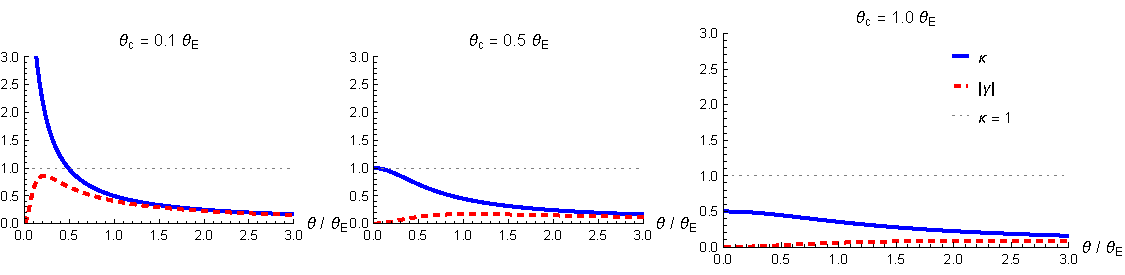
\includegraphics[width=0.85\textwidth]{../Figures/07_Axisymmetric_Models/nis_critical_curves.pdf}
    \caption{Effect of the core radius on the NIS convergence and
    shear, shown for three regimes that control the critical-curve
    topology.
    \textbf{Left:} for $\theta_c = 0.1\,\thetaE < \thetaE/2$, the
    central convergence $\kappab(0)>1$, so both tangential and radial
    critical curves exist and three images can form.
    \textbf{Center:} at the critical value $\theta_c = 0.5\,\thetaE =
    \thetaE/2$, $\kappab(0)=1$ exactly and the radial critical curve
    collapses to a point.
    \textbf{Right:} for $\theta_c = 1.0\,\thetaE > \thetaE/2$,
    $\kappab(0)<1$ everywhere; no critical curves exist and only one
    image forms.  Generated by
    \texttt{axisymmetric\_models.wl}.}
    \label{fig:nis_critical_curves}
\end{figure}


% =====================================================================
\section{NFW Profile}
\label{sec:nfw}

The \textbf{Navarro--Frenk--White} (NFW) profile is the ``universal''
dark matter halo density profile found in cosmological $N$-body
simulations (Navarro, Frenk \& White 1996, 1997).  It is the standard
model for the mass distribution of galaxy clusters and is essential
for cluster lensing (Module~10).

\subsection{Three-Dimensional Density Profile}

\begin{equation}
    \boxed{
    \rho(r) = \frac{\rho_s}{\left(\dfrac{r}{r_s}\right)
    \left(1 + \dfrac{r}{r_s}\right)^2}
    }
    \label{eq:nfw_rho}
\end{equation}
where $r_s$ is the \textbf{scale radius} and $\rho_s$ is a
characteristic density.  The profile has two regimes:
\begin{itemize}
    \item $r \ll r_s$: $\rho \propto r^{-1}$ (cusp, shallower than
          isothermal),
    \item $r \gg r_s$: $\rho \propto r^{-3}$ (steeper than
          isothermal, finite total mass within a virial radius).
\end{itemize}

\subsection{NFW Parameters: Concentration and Virial Mass}

The NFW profile is usually parametrized by two quantities:
\begin{itemize}
    \item The \textbf{virial mass} $M_{200}$: the mass enclosed
          within the virial radius $r_{200}$, defined as the radius
          within which the mean density is 200 times the critical
          density of the universe.
    \item The \textbf{concentration parameter}
          $c = r_{200}/r_s$: the ratio of virial to scale radius.
          Typical values are $c \sim 3$--$5$ for massive clusters
          ($M_{200} \sim 10^{15}\,\Msun$) and $c \sim 10$--$20$ for
          galaxy-mass haloes ($M_{200} \sim 10^{12}\,\Msun$).
\end{itemize}

The characteristic density is related to $c$ by:
\begin{equation}
    \rho_s = \frac{200}{3}\,\rho_{\mathrm{crit}}\,
    \frac{c^3}{\ln(1+c) - c/(1+c)} \,.
    \label{eq:nfw_rho_s}
\end{equation}

\subsection{Surface Mass Density of the NFW}
\label{sec:nfw_sigma}

The line-of-sight projection of the NFW density gives the surface mass
density
\begin{equation}
    \Sigma(\xi) \;=\; \int_{-\infty}^{\infty}
        \rho\!\left(\sqrt{\xi^2 + z^2}\right)\,dz \,,
    \label{eq:nfw_sigma_setup}
\end{equation}
where $\xi$ is the physical impact parameter in the lens plane and $z$
is the line-of-sight coordinate.  We now evaluate this integral
explicitly; the computation separates cleanly into three steps and is
the first place where the distinctive NFW branch structure
(arccosh vs.\ arctan) appears.  The full derivation is verified
symbolically in
\mathlink{07_Axisymmetric_Models/nfw\_projection.wl}{nfw\_projection.wl}.

\paragraph{Step 1: dimensionless variables.}
Let $x = \xi/r_s$ and $u = z/r_s$, so that $r/r_s = \sqrt{x^2+u^2}$ and
$dz = r_s\,du$.  The NFW density (eq.~\ref{eq:nfw_rho}) becomes
\begin{equation*}
    \rho = \frac{\rho_s}{\sqrt{x^2+u^2}\,\bigl(1 + \sqrt{x^2+u^2}\bigr)^2}\,.
\end{equation*}
Using the symmetry $z \leftrightarrow -z$,
\begin{equation}
    \Sigma(\xi) \;=\; 2\,\rho_s\,r_s\,I(x) \,,
    \qquad
    I(x) = \int_0^{\infty}\!
        \frac{du}{\sqrt{x^2+u^2}\,\bigl(1 + \sqrt{x^2+u^2}\bigr)^2}\,.
    \label{eq:nfw_I_definition}
\end{equation}

\paragraph{Step 2: change of variable $w = \sqrt{x^2+u^2}$.}
Then $u\,du = w\,dw$ and $du = w\,dw/\sqrt{w^2-x^2}$.  The limits
$u\!:\!0\to\infty$ map to $w\!:\!x\to\infty$, and
\begin{equation}
    I(x) \;=\; \int_{x}^{\infty}\!
        \frac{dw}{(1+w)^2\,\sqrt{w^2 - x^2}} \,.
    \label{eq:nfw_I_wform}
\end{equation}

\paragraph{Step 3: reduce to a simpler integral.}
A short calculation gives the identity
\begin{equation}
    \frac{d}{dw}\!\left[\frac{\sqrt{w^2-x^2}}{1+w}\right]
    \;=\;
    \frac{w + x^2}{(1+w)^2\sqrt{w^2-x^2}}\,.
    \label{eq:nfw_parts_identity}
\end{equation}
Writing $w + x^2 = (1+w) + (x^2 - 1)$ splits the right side into a
piece involving one power of $(1+w)$ in the denominator and the
target integrand $\bigl[(1+w)^2\sqrt{w^2-x^2}\bigr]^{-1}$ multiplied by
$(x^2-1)$.  Integrating eq.~\eqref{eq:nfw_parts_identity} from $w=x$ to
$w=\infty$ and using $\sqrt{w^2-x^2}/(1+w)\to 1$ at infinity and $0$ at
$w=x$:
\begin{equation}
    1 \;=\; K(x) \;+\; (x^2 - 1)\,I(x) \,,
    \qquad
    K(x) \equiv \int_x^{\infty}\!\frac{dw}{(1+w)\sqrt{w^2-x^2}}\,,
    \label{eq:nfw_IbK}
\end{equation}
so
\begin{equation}
    I(x) \;=\; \frac{1 - K(x)}{x^2 - 1}\,.
    \label{eq:nfw_I_as_K}
\end{equation}

\paragraph{Step 4: evaluate $K(x)$.}
The substitution $w = x\cosh\tau$ (with $\sqrt{w^2-x^2} = x\sinh\tau$,
$dw = x\sinh\tau\,d\tau$) turns $K$ into
\begin{equation}
    K(x) \;=\; \int_0^{\infty} \frac{d\tau}{1 + x\cosh\tau} \,,
    \label{eq:nfw_Ktau}
\end{equation}
which is elementary.  Using the Weierstrass half-angle substitution
$t = \tanh(\tau/2)$ and the standard result
$\int_0^1\! 2\,dt/(a-b\,t^2)
= (2/\sqrt{ab})\,\operatorname{arctanh}\!\sqrt{b/a}$
(and its arctan analog when the signs flip), one finds
\begin{equation}
    \boxed{
    K(x) = \begin{cases}
        \dfrac{\operatorname{arccosh}(1/x)}{\sqrt{1-x^2}},
            & 0 < x < 1, \\[8pt]
        1, & x = 1, \\[4pt]
        \dfrac{\arctan\!\sqrt{x^2-1}}{\sqrt{x^2-1}},
            & x > 1.
    \end{cases}}
    \label{eq:nfw_K_branches}
\end{equation}
The two branches are related by the identity
$\operatorname{arccosh}(1/x) \leftrightarrow \arccos(1/x)$ (analytic
continuation through $x=1$), and the $x=1$ value follows from a
Taylor expansion of either branch.

\paragraph{Collected result.}
Substituting eq.~\eqref{eq:nfw_K_branches} into
eq.~\eqref{eq:nfw_I_as_K}, and then eq.~\eqref{eq:nfw_I_definition},
\begin{equation}
    \boxed{
    \Sigma(x) = 2\,\rho_s\,r_s\, f(x)\,,
    \qquad
    f(x) = \frac{1 - K(x)}{x^2 - 1}\,,}
    \label{eq:nfw_sigma}
\end{equation}
where $x = \xi / r_s = \theta / \theta_s$ and $\theta_s = r_s / \Dd$.
Writing out the three branches explicitly,
\begin{equation}
    f(x) = \begin{cases}
    \dfrac{1}{x^2 - 1}\!\left(1 - \dfrac{\operatorname{arccosh}(1/x)}{\sqrt{1-x^2}}\right)
            & 0 < x < 1, \\[8pt]
    \dfrac{1}{3} & x = 1, \\[8pt]
    \dfrac{1}{x^2 - 1}\!\left(1 - \dfrac{\arctan\!\sqrt{x^2-1}}{\sqrt{x^2-1}}\right)
            & x > 1.
    \end{cases}
    \label{eq:nfw_f}
\end{equation}
This recovers the standard result of Bartelmann (1996) and
Wright \& Brainerd (2000).

\begin{remark}
The apparent singularity at $x = 1$ in eq.~\eqref{eq:nfw_f} cancels
between numerator and denominator.  A Taylor expansion of $1 - K(x)$
about $x = 1$ (for either branch) gives
$1 - K(x) = \tfrac{1}{3}(x^2 - 1) + \order{(x^2-1)^2}$, leaving
$f(1) = 1/3$ --- a smooth function of $x$.
\end{remark}

\subsection{Convergence of the NFW}

Dividing eq.~\eqref{eq:nfw_sigma} by the critical surface density,
\begin{equation}
    \boxed{
    \kappab(x) \;=\; \frac{\Sigma(x)}{\Sigmacr}
    \;=\; \frac{2\,\rho_s\,r_s}{\Sigmacr}\, f(x)
    \;\equiv\; \kappa_s\, f(x) \,,
    \qquad
    \kappa_s \equiv \frac{2\rho_s r_s}{\Sigmacr}.}
    \label{eq:nfw_kappa}
\end{equation}
The characteristic convergence $\kappa_s$ collects every
dimensionful quantity from the density profile and the distance
configuration, leaving $f(x)$ purely dimensionless.

\begin{remark}
Unlike the SIS (where $\kappab \propto \theta^{-1}$), the NFW
convergence has a \textit{logarithmic} divergence as $x \to 0$.  This
follows from the small-$x$ expansion of eq.~\eqref{eq:nfw_K_branches},
$\operatorname{arccosh}(1/x) = \ln(2/x) + \order{x^2}$, which gives
$K(x)\to \ln(2/x)$ and hence $f(x) \sim \ln(2/x)$ as $x\to 0$.  The
NFW cusp ($\rho \propto r^{-1}$) is shallower than the isothermal cusp
($\rho \propto r^{-2}$), which has important consequences for central
image formation.
\end{remark}

\subsection{Deflection Angle and Shear of the NFW}

For any axisymmetric profile, the reduced deflection angle satisfies
eqs.~\eqref{eq:mean_kappa} and~\eqref{eq:alpha_mean_kappa},
\begin{equation}
    \alpha(\theta) \;=\; \theta\,\bar\kappa(\theta) \,,
    \qquad
    \bar\kappa(\theta) = \frac{2}{\theta^2}\int_0^\theta
        \kappab(\theta')\,\theta'\,d\theta'.
    \label{eq:nfw_alpha_setup}
\end{equation}
Switching to $x = \theta/\theta_s$ and using
$\kappab = \kappa_s f(x)$ (eq.~\ref{eq:nfw_kappa}) turns the integral
into
\begin{equation}
    \bar\kappa(x) = \frac{2\kappa_s}{x^2}\,h(x) \,,
    \qquad
    h(x) \equiv \int_0^x f(x')\,x'\,dx'.
    \label{eq:nfw_hdef}
\end{equation}

\paragraph{Evaluation of $h(x)$.}
From eq.~\eqref{eq:nfw_I_as_K},
$f(x) = [1 - K(x)]/(x^2-1)$, where $K(x)$ is given by
eq.~\eqref{eq:nfw_K_branches}.  A direct calculation shows
\begin{equation}
    \frac{d}{dx}\!\left[\ln\!\tfrac{x}{2} + K(x)\right]
    \;=\; x\,f(x)
    \quad\text{for } 0 < x \neq 1,
    \label{eq:nfw_antiderivative}
\end{equation}
and, using
$\operatorname{arccosh}(1/x) = \ln(2/x) + \order{x^2}$ as $x \to 0$,
\begin{equation*}
    \lim_{x\to 0^+}\bigl[\ln(x/2) + K(x)\bigr] = 0 \,.
\end{equation*}
Hence
\begin{equation}
    h(x) \;=\; \ln\!\frac{x}{2} + g(x) \,,
    \qquad
    g(x) \equiv K(x),
    \label{eq:nfw_h_evaluated}
\end{equation}
with
\begin{equation}
    g(x) = \begin{cases}
        \dfrac{\operatorname{arccosh}(1/x)}{\sqrt{1-x^2}}, & 0 < x < 1, \\[6pt]
        1, & x = 1, \\[4pt]
        \dfrac{\arctan\!\sqrt{x^2-1}}{\sqrt{x^2-1}}, & x > 1.
    \end{cases}
    \label{eq:nfw_g}
\end{equation}

\paragraph{Deflection angle and shear.}
Substituting eq.~\eqref{eq:nfw_h_evaluated} into
eqs.~\eqref{eq:nfw_alpha_setup}--\eqref{eq:nfw_hdef} and using
$\theta = x\,\theta_s$:
\begin{equation}
    \boxed{
    \alpha(x) = \frac{2\kappa_s\,\theta_s}{x}\,
    \left[\ln\frac{x}{2} + g(x)\right],
    \qquad
    \bar\kappa(x) = \frac{2\kappa_s}{x^2}\,
    \left[\ln\frac{x}{2} + g(x)\right].}
    \label{eq:nfw_alpha}
\end{equation}
The tangential shear of any axisymmetric profile is
$|\gammaL(x)| = \bar\kappa(x) - \kappab(x)$
(cf.\ eq.~\ref{eq:gamma_circular}):
\begin{equation}
    |\gammaL(x)| \;=\; \frac{2\kappa_s}{x^2}
        \left[\ln\frac{x}{2} + g(x)\right]
        \;-\; \kappa_s\,f(x) \,.
    \label{eq:nfw_gamma}
\end{equation}
Every identity in this subsection --- the antiderivative
eq.~\eqref{eq:nfw_antiderivative}, the $x \to 0$ limit, and the
numerical consistency of eq.~\eqref{eq:nfw_alpha} with direct
integration of $\kappab$ --- is verified symbolically and numerically
in
\mathlink{07_Axisymmetric_Models/nfw\_projection.wl}{nfw\_projection.wl}.

\subsection{Role of Concentration in NFW Lensing}

The concentration parameter $c$ has a strong effect on the lensing
strength of an NFW halo:
\begin{itemize}
    \item Higher $c$ means more centrally concentrated mass, increasing
          the central convergence $\kappab(0)$ and making strong lensing
          more likely.
    \item For a fixed virial mass, increasing $c$ increases $\kappa_s$
          and decreases $\theta_s$, concentrating the lensing signal in
          a smaller angular region.
    \item Typical galaxy clusters ($c \sim 4$--$5$) are strong lenses
          for background sources at $z_s \gtrsim 1$, producing giant
          arcs with radii of $\sim 10''$--$30''$.
\end{itemize}

The NFW model will be applied extensively to cluster lensing in
Module~10.

\begin{figure}[ht]
    \centering
    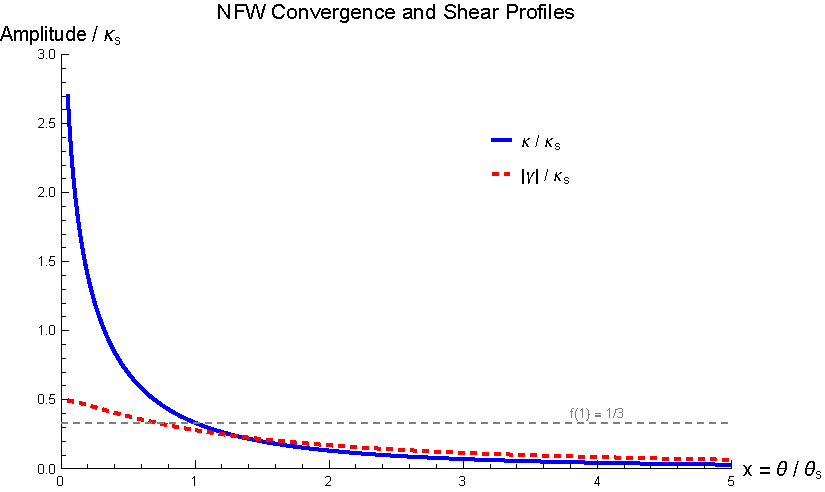
\includegraphics[width=0.75\textwidth]{../Figures/07_Axisymmetric_Models/nfw_profiles.pdf}
    \caption{NFW convergence $\kappab(x)/\kappa_s = f(x)$ (solid) and
    shear $|\gammaL(x)|/\kappa_s = \bar\kappa(x)/\kappa_s - f(x)$
    (dashed) as functions of the dimensionless radius $x = \theta/
    \theta_s$.  Both curves are normalized to $\kappa_s$ and are
    universal functions of $x$ (independent of concentration); the
    horizontal grey line marks $f(1) = 1/3$.  The concentration $c$
    enters only through the overall scale $\kappa_s$ and the angular
    scale $\theta_s$, both of which absorb the dependence on $c$ and
    on the cosmological distances.  Generated by
    \texttt{axisymmetric\_models.wl}.}
    \label{fig:nfw_profiles}
\end{figure}


% =====================================================================
\section{Comparison of Models}
\label{sec:model_comparison}

Table~\ref{tab:model_comparison} summarizes the key properties of the
four axisymmetric lens models covered in this module.

\begin{table}[ht]
\centering
\caption{Comparison of axisymmetric lens models.  Here
$\theta$ is the angular radius from the lens center in units of the
appropriate scale ($\thetaE$ for point mass and SIS, $\theta_s$ for
NFW).}
\label{tab:model_comparison}
\begin{tabular}{@{}lcccc@{}}
\toprule
Property & Point Mass & SIS & NIS & NFW \\
\midrule
$\rho(r)$ & $\delta^{(3)}$ & $\propto r^{-2}$ & $\propto (r^2+r_c^2)^{-1}$ & eq.~\eqref{eq:nfw_rho} \\[4pt]
$\kappab(\theta)$ & $0$ ($\theta \neq 0$) & $\thetaE / 2\theta$ & $\thetaE / 2\sqrt{\theta^2+\theta_c^2}$ & $\kappa_s\, f(x)$ \\[4pt]
$\alpha(\theta)$ & $\thetaE^2/\theta$ & $\thetaE$ & eq.~\eqref{eq:nis_alpha} & eq.~\eqref{eq:nfw_alpha} \\[4pt]
$\kappab = |\gammaL|$? & No ($\kappab=0$) & Yes & No & No \\[4pt]
Tangential CC & $\theta = \thetaE$ & $\theta = \thetaE$ & Yes & Yes \\[4pt]
Radial CC & No & No & Yes ($\theta_c < \thetaE/2$) & Yes \\[4pt]
Max images & 2 & 2 & 3 & 3 \\[4pt]
Caustic & Point & Point & Point $+$ circle & Point $+$ circle \\
\bottomrule
\end{tabular}
\end{table}

The key qualitative differences between the models are:

\begin{enumerate}
    \item \textbf{Central density:} The point mass and SIS have
          singular central densities; the NIS and NFW have finite (or
          logarithmically divergent) central densities.  The central
          density determines whether a radial critical curve can form.

    \item \textbf{Deflection angle behavior:} The point mass
          deflection $\alpha \propto 1/\theta$ diverges at the center
          and falls off with distance.  The SIS deflection is constant.
          The NIS and NFW deflections are intermediate.

    \item \textbf{Image multiplicity:} Models with a radial critical
          curve (NIS, NFW) can produce a third (central) image.  The
          SIS and point mass produce at most two images.

    \item \textbf{Asymptotic behavior:} The SIS has $\Sigma \propto
          \theta^{-1}$ and infinite total mass.  The NFW has
          $\Sigma \propto \theta^{-2}$ (for $\theta \gg \theta_s$) and
          a well-defined virial mass.
\end{enumerate}

\begin{figure}[ht]
    \centering
    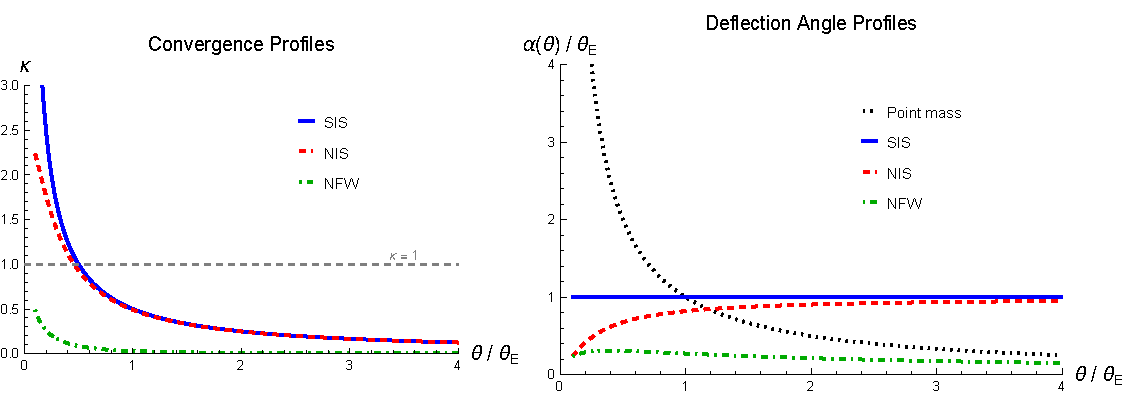
\includegraphics[width=0.85\textwidth]{../Figures/07_Axisymmetric_Models/model_comparison.pdf}
    \caption{Comparison of convergence profiles (left) and deflection
    angles (right) for the four axisymmetric models.  All curves use
    the SIS Einstein radius $\thetaE$ as the unit of length on the
    horizontal axis; the SIS, NIS and NFW amplitudes are set so that
    the profiles can be compared on the same panel
    (specifically NIS with $\theta_c = 0.2\,\thetaE$ and NFW with
    $\theta_s = 0.3\,\thetaE,\;\kappa_s = 0.5$).  Only the SIS and
    NIS are normalized to reproduce $\bar\kappa(\thetaE) = 1$; the
    NFW deflection therefore does not pass through $\alpha = \thetaE$
    at $\theta = \thetaE$ on this plot.  The point mass convergence
    is a delta function and is not shown.  Generated by
    \texttt{axisymmetric\_models.wl}.}
    \label{fig:model_comparison}
\end{figure}


% =====================================================================
\section{Summary}
\label{sec:axi_summary}

\begin{itemize}
    \item For a \textbf{circularly symmetric} lens, all quantities
          depend only on $\theta = |\vectheta|$.  The deflection angle
          is $\alpha(\theta) = \bar{\kappa}(\theta)\,\theta$, and the
          shear is $|\gammaL| = \bar{\kappa} - \kappab$.

    \item The \textbf{point mass} lens has $\alpha = \thetaE^2/\theta$,
          $\kappab = 0$ (away from origin), and always produces two
          images.

    \item The \textbf{SIS} has $\rho \propto r^{-2}$, a constant
          physical deflection angle
          $\alphahat = 4\pi\sigma_v^2/\speedoflight^2$, Einstein radius
          $\thetaE = 4\pi(\sigma_v/\speedoflight)^2\,\Dds/\Ds$, and
          $\kappab = |\gammaL| = \thetaE/(2\theta)$ everywhere.

    \item The SIS produces two images for $\beta < \thetaE$ and one
          image for $\beta > \thetaE$, with magnifications
          $\mu_\pm = 1 \pm \thetaE/\beta$.  It has a tangential
          critical curve (Einstein ring) but no radial critical curve.

    \item The \textbf{NIS} introduces a core radius $\theta_c$ that
          removes the central singularity.  For $\theta_c < \thetaE/2$,
          a radial critical curve appears, enabling a third (central)
          image.  The NIS reduces to the SIS for $\theta_c \to 0$.

    \item The \textbf{NFW} profile
          $\rho = \rho_s / [(r/r_s)(1+r/r_s)^2]$ is the universal dark
          matter halo profile.  It is parametrized by the virial mass
          $M_{200}$ and concentration $c$.  Higher concentration
          increases the lensing strength.

    \item Models with finite central density (NIS, NFW) possess a
          radial critical curve and can produce three images.  The
          SIS and point mass cannot.
\end{itemize}


% =====================================================================
\section{Problems}
\label{sec:axi_problems}

\begin{exercise}
\label{ex:sis_deflection_derivation}
\textbf{(Derivation of the SIS deflection angle.)}
Starting from the SIS density profile $\rho(r) = \sigma_v^2/(2\pi
\Gnewton r^2)$:
\begin{enumerate}[label=(\alph*)]
    \item Compute the surface mass density
          $\Sigma(\xi) = \int_{-\infty}^{+\infty}
          \rho(\sqrt{\xi^2 + z^2})\, dz$ and show that
          $\Sigma(\xi) = \sigma_v^2 / (2\Gnewton\,\xi)$.
          \textit{Hint:} Use the substitution $z = \xi\tan\phi$.
    \item Compute the projected enclosed mass
          $M(\xi) = 2\pi \int_0^\xi \Sigma(\xi')\,\xi'\,d\xi'$.
    \item Using $\alphahat(\xi) = 4\Gnewton M(\xi) /
          (\speedoflight^2\,\xi)$, show that
          $\alphahat = 4\pi\sigma_v^2/\speedoflight^2$, independent of
          $\xi$.
    \item Derive the SIS Einstein radius $\thetaE$.
\end{enumerate}
Verify with
\solnlink{07_Axisymmetric_Models/problems\_07.wl}{problems\_07.wl}.
\end{exercise}

\begin{exercise}
\label{ex:sis_kappa_equals_gamma}
\textbf{(SIS: $\kappab = |\gammaL|$ everywhere.)}
\begin{enumerate}[label=(\alph*)]
    \item For the SIS with $\kappab(\theta) = \thetaE/(2\theta)$,
          compute the mean convergence $\bar{\kappa}(\theta)$ using
          eq.~\eqref{eq:mean_kappa}.
    \item Show that $|\gammaL(\theta)| = \bar{\kappa}(\theta) -
          \kappab(\theta) = \thetaE/(2\theta) = \kappab(\theta)$.
    \item Explain physically why $\kappab = |\gammaL|$ for the SIS
          but $\kappab = 0 \neq |\gammaL|$ for the point mass.
          \textit{Hint:} Consider the mass distribution --- where is
          the mass located for each model?
    \item Show that for \textit{any} power-law profile
          $\kappab(\theta) \propto \theta^{-n}$ with $n > 0$, the
          ratio $|\gammaL|/\kappab$ is constant, and find the value of
          $n$ for which $|\gammaL| = \kappab$.
\end{enumerate}
Verify with
\solnlink{07_Axisymmetric_Models/problems\_07.wl}{problems\_07.wl}.
\end{exercise}

\begin{exercise}
\label{ex:sis_numerical}
\textbf{(SIS numerical example.)}
Consider an SIS lens with $\sigma_v = 250$~km\,s$^{-1}$ at
$z_d = 0.3$ lensing a source at $z_s = 1$.  Use
$\Dd \approx 920$~Mpc, $\Ds \approx 1650$~Mpc,
$\Dds \approx 1055$~Mpc.
\begin{enumerate}[label=(\alph*)]
    \item Compute the Einstein radius $\thetaE$ in arcseconds.
    \item For a source at $\beta = 0.5''$:
          \begin{enumerate}[label=(\roman*)]
              \item Is the source inside or outside the caustic?
              \item Find the image positions $\theta_+$ and $\theta_-$.
              \item Compute the magnifications $\mu_+$ and $\mu_-$.
              \item Compute the total magnification.
          \end{enumerate}
    \item For what source position $\beta$ does the SIS produce images
          with equal absolute magnification?  Is this physically
          realizable?
    \item Compare the SIS Einstein radius with the point mass Einstein
          radius for $M = 10^{12}\,\Msun$ at the same redshifts.
          Comment on the difference.
\end{enumerate}
Verify with
\solnlink{07_Axisymmetric_Models/problems\_07.wl}{problems\_07.wl}.
\end{exercise}

\begin{exercise}
\label{ex:nis_convergence}
\textbf{(NIS convergence and SIS limit.)}
\begin{enumerate}[label=(\alph*)]
    \item Starting from the NIS surface mass density
          $\Sigma(\theta) = \sigma_v^2 / [2\Gnewton\,\Dd\,
          \sqrt{\theta^2 + \theta_c^2}]$, derive the NIS convergence
          $\kappab(\theta) = \thetaE / [2\sqrt{\theta^2 + \theta_c^2}]$.
    \item Show that the NIS convergence reduces to the SIS convergence
          $\kappab = \thetaE/(2\theta)$ in the limit $\theta_c \to 0$.
    \item Find the critical value of $\theta_c$ (in terms of $\thetaE$)
          above which the NIS cannot produce multiple images.
          \textit{Hint:} multiple images require $\kappab(0) \geq 1$.
    \item For the NIS with $\theta_c = 0.1\,\thetaE$, compute
          $\kappab(0)$, $\kappab(\thetaE)$, and
          $\kappab(2\,\thetaE)$.
    \item Sketch (or plot) the NIS convergence profile for
          $\theta_c = 0$ (SIS), $\theta_c = 0.1\,\thetaE$,
          $\theta_c = 0.3\,\thetaE$, and $\theta_c = 0.5\,\thetaE$
          on the same axes.
\end{enumerate}
Verify with
\solnlink{07_Axisymmetric_Models/problems\_07.wl}{problems\_07.wl}.
\end{exercise}

\begin{exercise}
\label{ex:nfw_concentration}
\textbf{(NFW concentration and lensing strength.)}
\begin{enumerate}[label=(\alph*)]
    \item Using the NFW convergence formula
          $\kappab(x) = \kappa_s\,f(x)$ (eq.~\ref{eq:nfw_kappa}),
          plot $\kappab(x)/\kappa_s$ as a function of
          $x = \theta/\theta_s$ for $0.01 \leq x \leq 10$.
    \item For a cluster at $z_d = 0.3$ with $M_{200} = 10^{15}\,\Msun$
          and source at $z_s = 1$, compute $\kappa_s$ and $\theta_s$
          for $c = 5$, $c = 10$, and $c = 20$.
    \item Plot the convergence profiles $\kappab(\theta)$ (in arcsec)
          for the three concentrations on the same axes.  At what
          angular radius does $\kappab = 1$ for each case?
    \item Discuss how the concentration parameter affects:
          (i)~the Einstein radius, (ii)~the size of the region
          where $\kappab > 1$, and (iii)~the lensing cross-section
          for producing giant arcs.
\end{enumerate}
Use Mathematica to generate the plots.
See \mathlink{07_Axisymmetric_Models/axisymmetric_models.wl}{axisymmetric\_models.wl}
and \solnlink{07_Axisymmetric_Models/problems\_07.wl}{problems\_07.wl}.
\end{exercise}

% =============================================================================
% Module 8: Non-Axisymmetric Models and Critical Curves
% =============================================================================
% Sources: Congdon & Keeton Ch. 4.5 & 6.1, Narayan & Bartelmann Sec. 3.5,
%          Saha et al., Petters, Levine & Wambsganss (2001)
% Mathematica: ../Mathematica/08_Elliptical_Models_Caustics/
% =============================================================================

\chapter{Non-Axisymmetric Models and Critical Curves}
\label{ch:elliptical_models}

\begin{quote}
\textit{Breaking circular symmetry in the lens model produces the rich
phenomenology of strong lensing: quadruply imaged quasars, Einstein
crosses, giant luminous arcs.  The structure of critical curves and
caustics determines everything --- how many images form, where they
appear, how bright they are, and even which direction they face.}
\hfill --- adapted from Congdon \& Keeton (2018)
\end{quote}

\noindent
In Modules~\ref{ch:magnification} and~\ref{ch:axisymmetric_models} we
developed the Jacobian formalism for magnification and applied it to
axisymmetric lens models: the point mass and the singular isothermal
sphere (SIS).  These models have a continuous rotational symmetry that
makes the mathematics tractable but the phenomenology limited.  The SIS,
for instance, can produce at most two images of a point source, and its
critical curve is a perfect circle.

Real galaxies, however, are \textit{elliptical}.  Their mass
distributions have axis ratios $q \sim 0.5$--$0.9$, and they live in
environments that contribute external tidal shear.  Breaking circular
symmetry introduces qualitatively new phenomena:
\begin{itemize}[nosep]
    \item Critical curves deform from circles into ellipses and ovals.
    \item Caustics develop a \textbf{diamond (astroid)} shape with
          cusps and folds.
    \item Sources can be \textbf{quadruply imaged} (not just doubly),
          producing Einstein crosses and arcs.
    \item The \textbf{topology} of image configurations --- how many
          images exist, their parities, and their magnifications ---
          is entirely governed by the source's position relative to
          the caustic structure.
\end{itemize}

This module introduces the two workhorse non-axisymmetric models
(SIS + external shear and the singular isothermal ellipsoid) and then
develops the theory of critical curves, caustics, and image topology
in full detail.  The image topology section is the conceptual heart
of strong lensing theory.

\medskip
\noindent
\textbf{Companion Mathematica files:}
\begin{itemize}[nosep]
    \item \mathlink{08_Elliptical_Models_Caustics/critical\_curves\_caustics.wl}{critical\_curves\_caustics.wl}
          --- symbolic and numerical computation of critical curves
          and caustics for SIS+shear and SIE models; image position
          solver; figure generation for all module figures
    \item \mathlink{08_Elliptical_Models_Caustics/image\_configurations.nb}{image\_configurations.nb}
          --- interactive notebook: place a source on the source
          plane and watch images appear, colored by parity; animate
          caustic crossings; sliders for ellipticity and shear
\end{itemize}


% =====================================================================
\section{Introduction: Why Non-Axisymmetric Models Matter}
\label{sec:elliptical_intro}

The singular isothermal sphere (Module~\ref{ch:axisymmetric_models}) is
an excellent starting point for galaxy-scale lensing.  Its velocity
dispersion $\sigma_v$ maps directly onto observable galaxy kinematics,
and its Einstein radius $\thetaE = 4\pi\sigma_v^2 \Dds/(\speedoflight^2
\Ds)$ sets the angular scale of lensing.  But the SIS has a fundamental
limitation: perfect circular symmetry.

Observations of strong lens systems reveal:
\begin{enumerate}
    \item \textbf{Quadruple images} are common.  About 20--30\% of
          known galaxy-scale lens systems are quads (four bright images
          plus a faint central image), which an SIS cannot produce.
    \item \textbf{Giant luminous arcs} in galaxy clusters are
          tangentially stretched images that trace out the critical
          curves of the cluster potential.  These arcs are not perfect
          circles, implying the mass distribution is not axisymmetric.
    \item \textbf{Astrometric anomalies} in lens models require
          ellipticity and/or external shear to achieve acceptable fits.
\end{enumerate}

The simplest way to break axial symmetry is to add a constant
\textbf{external shear} to the SIS potential.  The resulting
SIS + shear model already captures the essential features: diamond
caustics, quad images, and fold/cusp configurations.  The more
physically motivated \textbf{singular isothermal ellipsoid} (SIE)
achieves the same through an intrinsically elliptical mass
distribution and is the model used in modern lens-modeling codes
such as \texttt{lenstronomy} and \texttt{PyAutoLens}.


% =====================================================================
\section{SIS + External Shear}
\label{sec:sis_shear}

The simplest non-axisymmetric lens model augments the SIS potential
with a constant external tidal shear $\gamma_{\mathrm{ext}}$.
Physically, this shear arises from the tidal gravitational field of
neighboring galaxies or the cluster environment in which the lens
galaxy resides.

\subsection{Lensing Potential}

The lensing potential is
(Congdon \& Keeton eq.~6.7):
\begin{equation}
    \boxed{
    \psiL(\vectheta) = \thetaE\,|\vectheta|
    + \frac{1}{2}\,\gamma_{\mathrm{ext}}\,
    (\theta_1^2 - \theta_2^2)
    }
    \label{eq:psi_sis_shear}
\end{equation}
where $|\vectheta| = \sqrt{\theta_1^2 + \theta_2^2}$ and we have
chosen the shear to be aligned with the $\theta_1$-axis (the general
case involves a rotation by the shear angle $\phi_\gamma$).  The
first term is the SIS potential; the second is the external shear
contribution.

\subsection{Deflection Angle}

The deflection angle components are:
\begin{equation}
    \alpha_1 = \frac{\partial\psiL}{\partial\theta_1}
    = \thetaE\,\frac{\theta_1}{|\vectheta|}
    + \gamma_{\mathrm{ext}}\,\theta_1 \,,
    \qquad
    \alpha_2 = \frac{\partial\psiL}{\partial\theta_2}
    = \thetaE\,\frac{\theta_2}{|\vectheta|}
    - \gamma_{\mathrm{ext}}\,\theta_2 \,.
    \label{eq:alpha_sis_shear}
\end{equation}
The SIS contribution deflects radially inward; the shear contribution
stretches along $\theta_1$ and compresses along $\theta_2$ (for
$\gamma_{\mathrm{ext}} > 0$).

\subsection{Convergence and Shear}

The convergence of the SIS + shear model is the same as the pure SIS
(the external shear does not add mass):
\begin{equation}
    \kappab(\vectheta) = \frac{\thetaE}{2\,|\vectheta|} \,.
    \label{eq:kappa_sis_shear}
\end{equation}
The total shear now has contributions from both the SIS and the
external shear.  For the SIS alone,
$|\gammaL_{\mathrm{SIS}}| = \thetaE/(2|\vectheta|) = \kappab$.
The external shear adds $\gamma_{\mathrm{ext}}$ aligned with the
coordinate axes, so the total shear field is anisotropic and
position-dependent.

\subsection{Critical Curves}

The critical curves are defined by $\det\Amat = 0$.  For the
SIS + shear model, the condition becomes (working in polar
coordinates $\theta_1 = \theta\cos\phi$,
$\theta_2 = \theta\sin\phi$):
\begin{equation}
    \boxed{
    \theta_{\mathrm{crit}}(\phi)
    = \frac{\thetaE}{1 - \gamma_{\mathrm{ext}}^2
    - 2\,\gamma_{\mathrm{ext}}\cos 2\phi}
    \cdot (1 - \gamma_{\mathrm{ext}}\cos 2\phi)
    }
    \label{eq:crit_sis_shear}
\end{equation}
For $\gamma_{\mathrm{ext}} = 0$ this reduces to $\theta = \thetaE$
(the SIS critical circle).  For $\gamma_{\mathrm{ext}} > 0$, the
critical curve is an \textbf{ellipse}: elongated along the
$\theta_2$-axis (perpendicular to the shear direction) and compressed
along $\theta_1$.

\begin{remark}
The critical curve is elongated \textit{perpendicular} to the shear
direction.  This is physically intuitive: the shear stretches images
along $\theta_1$, which means the magnification diverges at smaller
$\theta$ in that direction, pushing the critical curve inward along
$\theta_1$ and outward along $\theta_2$.
\end{remark}

\subsection{Caustics: The Diamond (Astroid)}

The caustics are obtained by mapping the critical curves through the
lens equation $\vecbeta = \vectheta_{\mathrm{crit}} -
\vecalpha(\vectheta_{\mathrm{crit}})$.  For the SIS + shear model,
the tangential caustic takes the shape of a \textbf{diamond} or
\textbf{astroid} --- a four-cusped curve.

In parametric form, the caustic is:
\begin{align}
    \beta_1(\phi) &= \theta_{\mathrm{crit}}(\phi)\cos\phi
    - \thetaE\cos\phi - \gamma_{\mathrm{ext}}\,
    \theta_{\mathrm{crit}}(\phi)\cos\phi \,,
    \label{eq:caustic_sis_shear_1} \\
    \beta_2(\phi) &= \theta_{\mathrm{crit}}(\phi)\sin\phi
    - \thetaE\sin\phi + \gamma_{\mathrm{ext}}\,
    \theta_{\mathrm{crit}}(\phi)\sin\phi \,.
    \label{eq:caustic_sis_shear_2}
\end{align}
This curve has four cusps (at $\phi = 0, \pi/2, \pi, 3\pi/2$) and
four fold segments connecting them.  The size of the diamond is
proportional to $\gamma_{\mathrm{ext}}$: for
$\gamma_{\mathrm{ext}} = 0$, the caustic degenerates to a point
(the SIS point caustic), and for larger shear values, the diamond
grows.

\begin{figure}[ht]
    \centering
    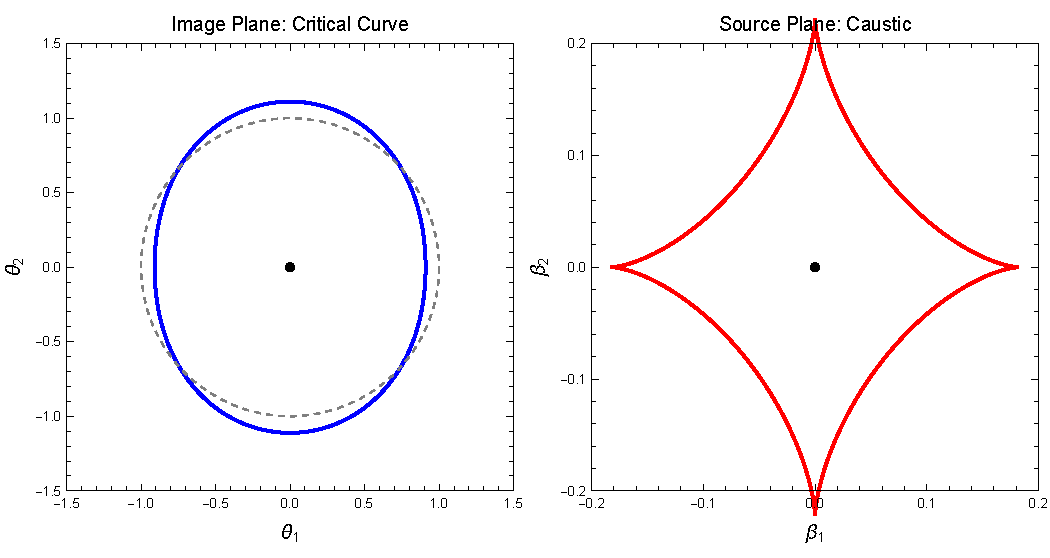
\includegraphics[width=0.85\textwidth]{../Figures/08_Elliptical_Models_Caustics/sis_shear_critical_caustic.pdf}
    \caption{Critical curves (left, image plane) and caustics (right,
    source plane) for the SIS + external shear model with
    $\thetaE = 1''$ and $\gamma_{\mathrm{ext}} = 0.1$.  The critical
    curve is an ellipse; the caustic is a diamond (astroid) with four
    cusps.  The shear axis is horizontal.
    Generated by \texttt{critical\_curves\_caustics.wl}.}
    \label{fig:sis_shear_crit_caust}
\end{figure}

\subsection{Image Configurations}

The image configurations for the SIS + shear model depend on the
source position relative to the diamond caustic:
\begin{itemize}
    \item \textbf{Source outside the diamond:} Two images (a double).
          One image is outside the critical curve (Type~I, positive
          parity); the other is inside (Type~II, negative parity,
          demagnified).
    \item \textbf{Source inside the diamond:} Four images (a quad).
          Two images outside the critical curve (positive parity);
          two inside (negative parity).
    \item \textbf{Source on a fold:} Three images, with two of them
          merging on the critical curve (highly magnified).
    \item \textbf{Source on a cusp:} Three images, with the merging
          triplet producing a characteristic cusp configuration.
\end{itemize}

\begin{remark}
The SIS is singular, so there is no separate radial critical curve
or radial caustic.  The SIS + shear model therefore has only a
tangential caustic (the diamond).  A non-singular model (e.g., a
softened isothermal sphere + shear) would also have a radial caustic
enclosing the tangential one.
\end{remark}


% =====================================================================
\section{The Singular Isothermal Ellipsoid (SIE)}
\label{sec:sie}

The \textbf{singular isothermal ellipsoid} (SIE) is the workhorse
model for galaxy-scale strong lensing.  Rather than adding shear
externally, the SIE builds ellipticity directly into the mass
distribution.

\subsection{Surface Mass Density}

The SIE surface mass density is
(Kormann, Schneider \& Bartelmann 1994; Congdon \& Keeton eq.~6.15):
\begin{equation}
    \boxed{
    \Sigma(\xi_1, \xi_2)
    = \frac{\sigma_v^2}{2\Gnewton}
    \,\frac{\sqrt{q}}{\sqrt{\xi_1^2 + q^2\,\xi_2^2}}
    }
    \label{eq:sie_sigma}
\end{equation}
where $q \leq 1$ is the axis ratio ($q = b/a$, with $a$ the
semi-major axis aligned along $\xi_1$), $\sigma_v$ is the velocity
dispersion, and $(\xi_1, \xi_2)$ are physical coordinates in the
lens plane.  For $q = 1$ this reduces to the SIS surface mass
density $\Sigma = \sigma_v^2/(2\Gnewton\xi)$.

The iso-density contours are ellipses with axis ratio $q$.  The
factor $\sqrt{q}$ ensures that the total mass enclosed within a
given elliptical radius is consistent with the isothermal profile.

\subsection{Deflection Angle}

The deflection angle for the SIE was derived by Kormann et al.\ (1994)
and involves inverse trigonometric/hyperbolic functions:
\begin{equation}
    \boxed{
    \alpha_1 = \frac{\thetaE\,\sqrt{q}}{\sqrt{1 - q^2}}
    \,\mathrm{arctan}\!\left(
    \frac{\theta_1\,\sqrt{1 - q^2}}
    {\sqrt{q^2\theta_1^2 + \theta_2^2}}\right)
    }
    \label{eq:sie_alpha1}
\end{equation}
\begin{equation}
    \boxed{
    \alpha_2 = \frac{\thetaE\,\sqrt{q}}{\sqrt{1 - q^2}}
    \,\mathrm{arctanh}\!\left(
    \frac{\theta_2\,\sqrt{1 - q^2}}
    {\sqrt{q^2\theta_1^2 + \theta_2^2}}\right)
    }
    \label{eq:sie_alpha2}
\end{equation}
where $\thetaE = 4\pi\sigma_v^2\Dds/(\speedoflight^2\Ds)$ is the
Einstein radius of the corresponding SIS\@.  Note the asymmetry:
$\alpha_1$ involves $\mathrm{arctan}$ while $\alpha_2$ involves
$\mathrm{arctanh}$.  This asymmetry reflects the elliptical geometry.

\begin{remark}
For $q \to 1$ (circular limit), both deflection components reduce to
$\alpha_i \to \thetaE\,\theta_i/|\vectheta|$, recovering the SIS
result.  This can be verified by taking the limit
$\sqrt{1-q^2} \to 0$ and using $\mathrm{arctan}(x)/x \to 1$ and
$\mathrm{arctanh}(x)/x \to 1$ as $x \to 0$.
\end{remark}

\subsection{Critical Curves and Caustics of the SIE}

The critical curves of the SIE are found by solving
$\det\Amat(\vectheta) = 0$.  Unlike the SIS (where the critical
curve is a circle), the SIE critical curves are smooth oval curves
whose shape depends on $q$.

For axis ratios $q \lesssim 0.9$, the SIE has:
\begin{itemize}
    \item A \textbf{tangential critical curve}: a smooth oval close
          to the Einstein radius, elongated perpendicular to the
          mass distribution's major axis.
    \item A \textbf{tangential caustic}: a diamond (astroid) shape,
          similar to the SIS + shear case, with four cusps.
\end{itemize}

The SIE, being singular at the origin, does not have a radial
critical curve (just as the SIS does not).  A non-singular
isothermal ellipsoid would also have a radial critical curve mapping
to a radial caustic.

The cross-section for quad lensing (the area enclosed by the
tangential caustic) increases with ellipticity.  For $q = 0.7$, the
caustic area is roughly $0.04\,\thetaE^2$, while for $q = 0.5$ it
can be several times larger.  This is why more elliptical galaxies
are more likely to produce quad lens systems.

\begin{figure}[ht]
    \centering
    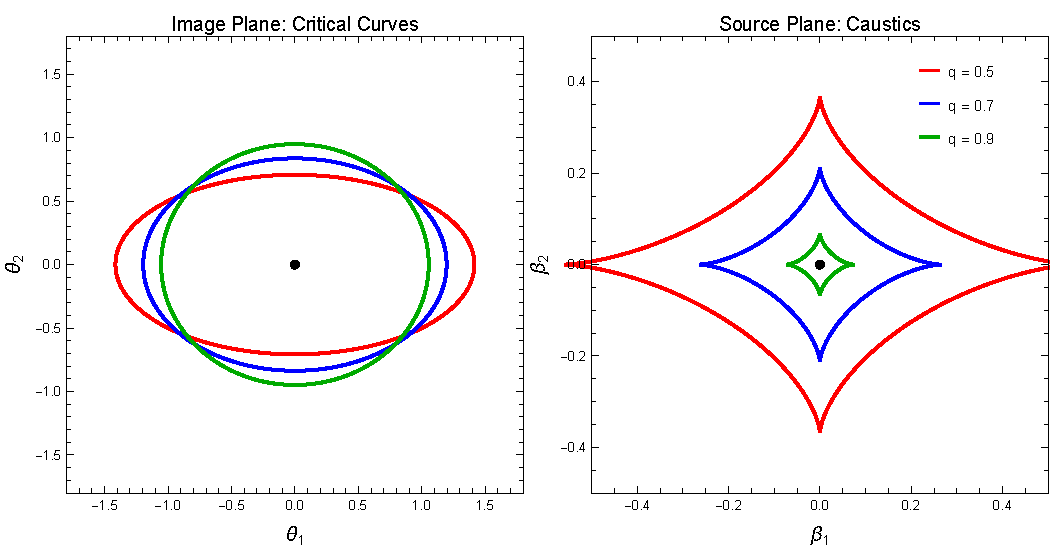
\includegraphics[width=0.85\textwidth]{../Figures/08_Elliptical_Models_Caustics/sie_critical_caustic.pdf}
    \caption{Critical curves (left) and caustics (right) for the SIE
    model with $\thetaE = 1''$ and axis ratios $q = 0.5$, $0.7$,
    and $0.9$.  As $q$ decreases (more elliptical), the diamond
    caustic grows larger, increasing the cross-section for
    quad imaging.
    Generated by \texttt{critical\_curves\_caustics.wl}.}
    \label{fig:sie_crit_caust}
\end{figure}


% =====================================================================
\section{Critical Curves}
\label{sec:critical_curves}

We now develop the general theory of critical curves, building on
the preview in Module~\ref{ch:magnification}
(Section~\ref{sec:critical_curves_preview}).

\begin{definition}
The \textbf{critical curves} are the loci in the image plane where
the Jacobian determinant vanishes:
\begin{equation}
    \boxed{
    \det\Amat(\vectheta) = 0
    \qquad \Longleftrightarrow \qquad
    (1 - \kappab)^2 - |\gammaL|^2 = 0
    }
    \label{eq:critical_curve_def}
\end{equation}
Equivalently, $\mu(\vectheta) \to \infty$ on critical curves.
\end{definition}

\subsection{Two Families of Critical Curves}

Using the eigenvalues $\lambda_\pm = 1 - \kappab \pm |\gammaL|$ of
the Jacobian (Module~\ref{ch:magnification}, eq.~\ref{eq:eigenvalues}),
the condition $\det\Amat = \lambda_+\,\lambda_- = 0$ is satisfied
when either eigenvalue vanishes:

\begin{enumerate}
    \item \textbf{Tangential critical curve} ($\lambda_- = 0$):
    \begin{equation}
        1 - \kappab(\vectheta) = |\gammaL(\vectheta)|
        \label{eq:tangential_crit}
    \end{equation}
    Images near this curve are stretched \textit{tangentially}
    (along the curve), because the eigenvalue corresponding to the
    tangential direction vanishes.  Giant arcs in clusters trace the
    tangential critical curve.

    \item \textbf{Radial critical curve} ($\lambda_+ = 0$):
    \begin{equation}
        1 - \kappab(\vectheta) = -|\gammaL(\vectheta)|
        \label{eq:radial_crit}
    \end{equation}
    Images near this curve are stretched \textit{radially}
    (perpendicular to the curve).  Radial arcs (pointing toward the
    lens center) form near radial critical curves, though they are
    rarer and fainter than tangential arcs.
\end{enumerate}

\subsection{Critical Curves for Axisymmetric vs.\ Elliptical Lenses}

\begin{itemize}
    \item \textbf{Axisymmetric lenses:} The critical curves are
          circles centered on the lens.  For the SIS, there is only
          a tangential critical curve at $\theta = \thetaE$.  For
          the point mass, the critical curve is the Einstein ring.
    \item \textbf{Elliptical lenses:} The critical curves become
          ellipses or ovals.  The tangential critical curve is
          typically elongated perpendicular to the lens ellipticity
          axis.  The shapes are computed numerically by solving
          $\det\Amat = 0$ on a grid or parametrically.
\end{itemize}

\subsection{Physical Meaning}

Critical curves are the sites of maximum magnification.  Images that
form near a critical curve are:
\begin{enumerate}
    \item \textbf{Highly magnified:} $|\mu| \gg 1$, because
          $\det\Amat \approx 0$.
    \item \textbf{Highly stretched:} Along one direction (tangential
          or radial), the magnification diverges while it remains
          finite in the orthogonal direction.  This produces the
          elongated arc morphology.
    \item \textbf{On parity boundaries:} As we cross a critical
          curve, $\det\Amat$ changes sign, so the image parity
          flips.  One side has positive parity (Type~I); the other
          has negative parity (Type~II).
\end{enumerate}

The practical significance is enormous: critical curves are where we
look for the most highly magnified background sources.  Cluster
lensing surveys map out critical curves to find magnified galaxies at
very high redshift.


% =====================================================================
\section{Caustics}
\label{sec:caustics}

\begin{definition}
The \textbf{caustics} are the images of the critical curves under the
lens mapping.  That is, the caustics are the curves in the
\textit{source plane} obtained by applying the lens equation to each
point on a critical curve:
\begin{equation}
    \boxed{
    \vecbeta_{\mathrm{caustic}}
    = \vectheta_{\mathrm{crit}}
    - \vecalpha(\vectheta_{\mathrm{crit}})
    }
    \label{eq:caustic_def_mod8}
\end{equation}
\end{definition}

\subsection{Types of Caustics}

Corresponding to the two families of critical curves, there are two
types of caustics:

\begin{enumerate}
    \item \textbf{Tangential caustic:} The mapping of the tangential
          critical curve.  For elliptical lenses, this is typically a
          diamond (astroid) shape with four cusps.  Sources inside
          the tangential caustic are quadruply imaged.

    \item \textbf{Radial caustic:} The mapping of the radial
          critical curve.  This is typically a smooth, roughly
          elliptical curve that encloses the tangential caustic.
          Sources inside the radial caustic but outside the
          tangential caustic are doubly imaged; sources outside both
          caustics have a single image.
\end{enumerate}

\subsection{Caustics for Specific Models}

\begin{itemize}
    \item \textbf{Point mass:} The tangential critical curve (Einstein
          ring $\theta = \thetaE$) maps to a single point
          ($\beta = 0$) --- a \textbf{degenerate point caustic}.  A
          source at $\beta = 0$ produces the Einstein ring; any
          source at $\beta > 0$ produces exactly two images.

    \item \textbf{SIS:} Same as the point mass --- the critical curve
          $\theta = \thetaE$ maps to $\beta = 0$.  The SIS has no
          radial caustic.  Sources with $\beta < \thetaE$ produce two
          images; sources with $\beta > \thetaE$ produce one image.

    \item \textbf{SIS + shear:} The tangential caustic opens up into
          a diamond (astroid) with four cusps.  The diamond size is
          proportional to $\gamma_{\mathrm{ext}}$.

    \item \textbf{SIE:} Same diamond structure as SIS + shear, with
          the diamond size controlled by the ellipticity $(1 - q)$.

    \item \textbf{Non-singular models} (NIS, NFW): Both tangential
          and radial caustics are present.  The radial caustic
          encloses the tangential one, creating regions with 1, 3,
          and 5 images.
\end{itemize}


% =====================================================================
\section{Image Topology}
\label{sec:image_topology}

This section is the conceptual heart of strong gravitational lensing.
It explains \textit{why} images appear and disappear as a source
moves, why they always come in pairs, and how the full image
configuration (positions, parities, magnifications) is determined
entirely by the source's location relative to the caustic structure.

The key insight is that \textbf{caustics are the boundaries between
regions of different image multiplicity}, and \textbf{critical curves
are the boundaries between regions of different image parity}.
Together, they provide a complete topological description of the
lens mapping.


\subsection{Critical Curves as Parity Boundaries}
\label{sec:parity_boundaries}

Recall from Module~\ref{ch:magnification} that the magnification is
$\mu = 1/\det\Amat$ and that the sign of $\mu$ determines the image
parity:
\begin{itemize}
    \item $\det\Amat > 0 \;\Rightarrow\; \mu > 0$: \textbf{positive
          parity} (Type~I image).  The image has the same orientation
          as the source.
    \item $\det\Amat < 0 \;\Rightarrow\; \mu < 0$: \textbf{negative
          parity} (Type~II image).  The image is mirror-reflected
          relative to the source.
\end{itemize}

Since $\det\Amat$ is a continuous function of position that passes
through zero on critical curves, the sign of $\det\Amat$ must
\textit{change} across a critical curve.  Therefore:

\begin{proposition}
\textbf{Critical curves are parity boundaries.}  Images on opposite
sides of a critical curve have opposite parities.  If a critical
curve separates region $R_+$ ($\det\Amat > 0$) from region $R_-$
($\det\Amat < 0$), then:
\begin{itemize}
    \item Images in $R_+$ have positive parity (Type~I, minima of the
          arrival time surface).
    \item Images in $R_-$ have negative parity (Type~II, saddle points
          of the arrival time surface).
\end{itemize}
\end{proposition}

For a typical galaxy lens with an elliptical mass distribution:
\begin{itemize}
    \item The region \textbf{outside} the tangential critical curve
          has $\det\Amat > 0$: images here are Type~I (positive
          parity, time-delay minima).
    \item The region \textbf{between} the tangential and radial
          critical curves has $\det\Amat < 0$: images here are
          Type~II (negative parity, saddle points).
    \item The region \textbf{inside} the radial critical curve has
          $\det\Amat > 0$ again: images here are Type~I or Type~III
          (positive parity, but corresponding to time-delay maxima
          for Type~III, as discussed in Module~\ref{ch:fermat_time_delays}).
\end{itemize}

\begin{remark}
The connection to Morse theory (Module~\ref{ch:fermat_time_delays})
is direct.  The three image types correspond to the three types of
stationary points of the Fermat potential: \textbf{Type~I} = minimum,
\textbf{Type~II} = saddle, \textbf{Type~III} = maximum.  The
magnification parity determines the Morse index.
\end{remark}


\subsection{Caustic Crossings and Image Creation/Destruction}
\label{sec:caustic_crossings}

The most important property of caustics is:

\begin{proposition}
\textbf{Image creation/destruction at caustics.}  When a source
crosses a caustic, the number of images changes by exactly two.  A
pair of images either \textbf{appears} (as the source enters a
higher-multiplicity region) or \textbf{disappears} (as it exits).
\end{proposition}

This happens because, as a source approaches a caustic from the side
with fewer images, two of the ``potential'' image positions on
opposite sides of the corresponding critical curve converge toward
the critical curve.  At the moment the source is exactly on the
caustic, the two images merge \textit{on} the critical curve (where
$\det\Amat = 0$ and the magnification diverges).  As the source
crosses the caustic, the two images separate and become distinct.

Crucially, the two images that appear or disappear:
\begin{enumerate}
    \item Are located on \textbf{opposite sides} of the critical
          curve.
    \item Have \textbf{opposite parities} (one Type~I, one Type~II).
    \item Are both \textbf{highly magnified} near the caustic
          (their magnifications diverge as they approach the critical
          curve).
    \item Have \textbf{nearly equal magnifications} (in absolute
          value) near the caustic.
\end{enumerate}

\begin{remark}
The fact that images always appear or disappear in \textbf{pairs}
with opposite parities is a topological necessity.  It preserves
\textbf{Burke's odd-number theorem}
(Module~\ref{ch:fermat_time_delays}): the total number of images is
always odd (for a non-singular, transparent lens with a source
inside the outermost caustic).  Since images are created and
destroyed in pairs, the parity of the count (odd or even) never
changes.
\end{remark}


\subsection{Walking a Source Across Caustics: A Worked Example}
\label{sec:source_walk}

To make the image creation/destruction process concrete, we walk
through a complete example using an SIE lens with axis ratio
$q = 0.7$ and Einstein radius $\thetaE = 1''$.  The SIE has a
tangential caustic (diamond shape) in the source plane.  For a
non-singular model there would also be a radial caustic enclosing
the diamond, but for the SIE (which is singular at the center) we
focus on the tangential caustic.

Consider a source that starts far from the lens and moves inward,
crossing the caustics:

\paragraph{Stage 1: Source far outside all caustics.}
The source position $\vecbeta$ is far from the lens center, well
outside any caustic.  There is \textbf{one image} (for singular
models like the SIE, there are actually two images even here, but
the second is extremely demagnified near the lens center and is
often unobservable).  The observable image is:
\begin{itemize}
    \item \textbf{Type~I} (positive parity, minimum of the arrival
          time).
    \item Located outside the tangential critical curve, near the
          true source position.
    \item Weakly magnified ($|\mu| \approx 1$).
\end{itemize}

\paragraph{Stage 2: Source crosses the tangential caustic (outside
$\to$ inside).}
As the source reaches the tangential (diamond) caustic, two new
images appear simultaneously, straddling the tangential critical
curve.  The total count goes from \textbf{1 to 3 images}
(or effectively from 2 to 4, counting the faint central image):
\begin{enumerate}
    \item The \textbf{original Type~I image} (positive parity,
          outside the tangential critical curve) persists, moving
          slightly.
    \item A \textbf{new Type~II image} (negative parity) appears
          just inside the tangential critical curve.  This is a
          \textit{saddle point} of the arrival time surface.  It is
          highly magnified and tangentially stretched.
    \item A \textbf{new Type~I image} (positive parity) appears
          just outside the tangential critical curve, close to the
          Type~II image.  This is a \textit{minimum} of the
          arrival time surface.  It is also highly magnified.
\end{enumerate}

The two new images are born as a highly magnified, closely spaced
pair straddling the critical curve.  They have opposite parities
(one positive, one negative) and nearly equal $|\mu|$.  As the
source moves further inside the caustic, they separate and their
magnifications decrease.

\paragraph{Stage 3: Source inside the tangential caustic (quad
configuration).}
With the source well inside the diamond caustic, four bright images
surround the lens (plus a faint, highly demagnified central image in
non-singular models).  The typical configuration is an
\textbf{Einstein cross}:
\begin{itemize}
    \item Two Type~I images (positive parity, outside the tangential
          critical curve).
    \item Two Type~II images (negative parity, inside the tangential
          critical curve).
\end{itemize}

The four images form a roughly cross-shaped pattern around the lens.
The magnification depends on the source's proximity to the caustic
folds and cusps.

\paragraph{Stage 4: Source crosses the tangential caustic again
(inside $\to$ outside).}
As the source exits the diamond caustic, two images converge on the
critical curve, merge, and disappear.  The count drops from
\textbf{3 back to 1} (or 4 to 2 counting the central image).  The
two images that disappear are a Type~I/Type~II pair, just as in the
creation event.

\begin{figure}[ht]
    \centering
    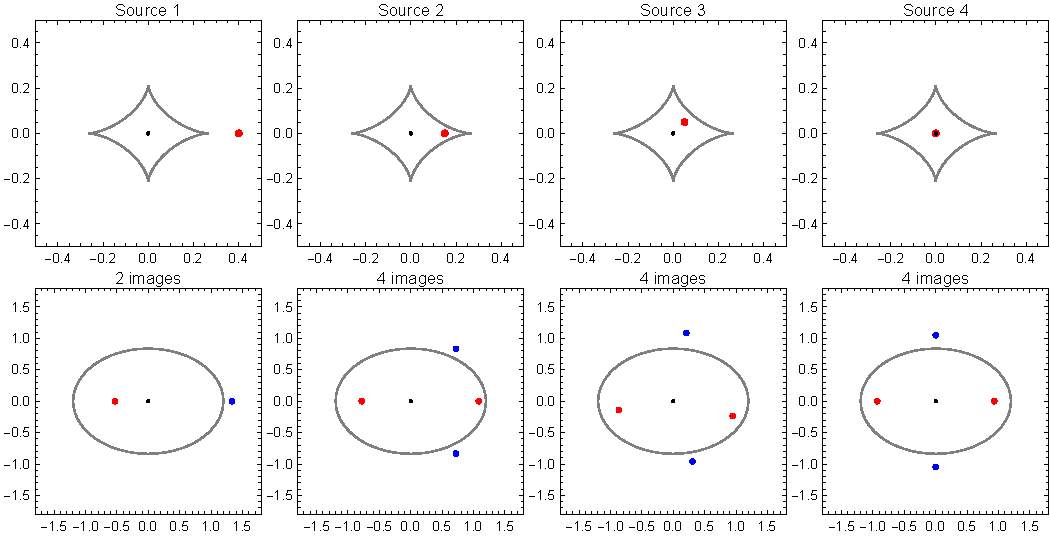
\includegraphics[width=0.95\textwidth]{../Figures/08_Elliptical_Models_Caustics/source_walk_caustic.pdf}
    \caption{A source walks across the caustic of an SIE lens
    ($q = 0.7$).  \textbf{Top row:} Source positions (red star) in
    the source plane, with the diamond caustic shown.
    \textbf{Bottom row:} Corresponding image configurations in the
    image plane, with the critical curve shown.  Blue circles =
    Type~I images (positive parity); red squares = Type~II images
    (negative parity).  As the source crosses the caustic, images
    appear/disappear in pairs.
    Generated by \texttt{critical\_curves\_caustics.wl}.}
    \label{fig:source_walk}
\end{figure}

For a non-singular lens model (e.g., a softened isothermal
ellipsoid), there is also a \textbf{radial caustic} enclosing the
tangential one.  As the source crosses the radial caustic inward,
two additional images appear near the radial critical curve (near
the lens center), bringing the total from 3 to 5.  This gives the
complete sequence:
\begin{center}
\begin{tabular}{ccccc}
\toprule
\textbf{Region} & \textbf{Image count} & \textbf{Types} \\
\midrule
Outside radial caustic & 1 & I \\
Between radial \& tangential & 3 & I, II, III \\
Inside tangential caustic & 5 & I, I, II, II, III \\
\bottomrule
\end{tabular}
\end{center}
Here Type~III is a maximum of the arrival time (the highly
demagnified central image).


\subsection{The Fold and Cusp Catastrophes}
\label{sec:fold_cusp}

The caustic curves of a generic smooth lens consist of two types of
points: \textbf{folds} (smooth segments) and \textbf{cusps} (pointed
corners).  These are the only two generic singularities of smooth
two-dimensional mappings, a result from \textbf{catastrophe theory}
(or singularity theory; see Petters, Levine \& Wambsganss 2001 for
a thorough treatment).

\subsubsection{Fold Caustics}

Near a \textbf{fold} (a smooth segment of the caustic), the
following properties hold:

\begin{enumerate}
    \item \textbf{Two images merge.}  As a source crosses a fold
          caustic, two images appear or disappear.  The images
          straddle the critical curve, one on each side.

    \item \textbf{Magnification scaling.}  Near a fold, the
          magnification of each of the two merging images scales as:
    \begin{equation}
        \boxed{
        |\mu| \propto \frac{1}{\sqrt{d_{\perp}}}
        }
        \label{eq:fold_magnification}
    \end{equation}
    where $d_\perp$ is the perpendicular distance of the source
    from the caustic.  The magnification diverges as
    $d_\perp \to 0$ (source on the caustic), but only as an
    inverse square root --- a relatively mild divergence.

    \item \textbf{Equal and opposite magnifications.}  The two
          merging images have magnifications that approach
          $+|\mu_0|$ and $-|\mu_0|$ (equal absolute values,
          opposite signs), so their \textit{total signed
          magnification} approaches zero.  The unsigned total
          $2|\mu_0| \propto 1/\sqrt{d_\perp}$ diverges.

    \item \textbf{Tangential stretching.}  The merging images are
          highly elongated tangentially (along the critical curve)
          and compressed radially.  This is the origin of the
          ``arc'' morphology.
\end{enumerate}

\subsubsection{Cusp Caustics}

Near a \textbf{cusp} (a pointed corner of the caustic), the behavior
is richer:

\begin{enumerate}
    \item \textbf{Three images merge.}  As a source approaches a
          cusp from inside the caustic, three images converge toward
          a single point on the critical curve.  These form the
          characteristic \textbf{cusp triplet}.

    \item \textbf{Stronger magnification divergence.}  Near a cusp,
          the total magnification diverges more strongly than for a
          fold.  The scaling is:
    \begin{equation}
        \mu_{\mathrm{total}} \propto d_{\perp}^{-1}
        \label{eq:cusp_magnification}
    \end{equation}
    (compared to $d_\perp^{-1/2}$ for a fold).

    \item \textbf{Cusp relation.}  The magnifications of the three
          cusp images satisfy a relation:
    \begin{equation}
        \mu_A + \mu_B + \mu_C \approx 0
        \label{eq:cusp_relation}
    \end{equation}
    where $A$, $B$, $C$ are the three images of the cusp triplet
    (with signed magnifications).  That is, the sum of the signed
    magnifications of the three brightest images in a cusp
    configuration should vanish.  Violations of this relation
    indicate substructure (e.g., dark matter subhalos) perturbing
    the images.

    \item \textbf{Configuration.}  The three cusp images are
          closely spaced along the critical curve.  One is on the
          opposite side of the critical curve from the other two,
          ensuring opposite parities.
\end{enumerate}

\begin{remark}
The fold and cusp are the only \textbf{stable} (generic)
singularities of smooth two-dimensional maps.  Higher-order
singularities (swallowtails, lips, etc.)\ require special symmetries
or fine-tuning and are not generically present in gravitational lens
models.  This is a deep result of Whitney's theorem in singularity
theory (Petters et al.\ 2001, Ch.~5--6).
\end{remark}

\begin{figure}[ht]
    \centering
    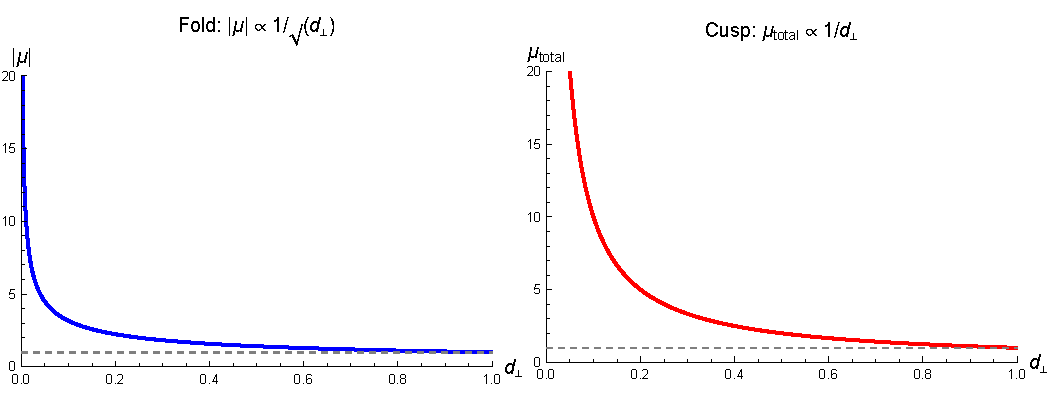
\includegraphics[width=0.85\textwidth]{../Figures/08_Elliptical_Models_Caustics/fold_cusp_magnification.pdf}
    \caption{Magnification behavior near fold and cusp caustics.
    \textbf{Left:} Near a fold, two images straddle the critical
    curve with magnifications scaling as $|\mu| \propto
    1/\sqrt{d_\perp}$.
    \textbf{Right:} Near a cusp, three images merge, with stronger
    divergence.  The cusp relation $\mu_A + \mu_B + \mu_C \approx 0$
    holds for the signed magnifications.
    Generated by \texttt{critical\_curves\_caustics.wl}.}
    \label{fig:fold_cusp}
\end{figure}


\subsection{Image Configuration Taxonomy}
\label{sec:image_taxonomy}

The caustic structure of a lens determines all possible image
configurations.  For an elliptical galaxy lens (SIE or similar model),
the following taxonomy applies:

\subsubsection{Doubles}

\textbf{Source outside the tangential caustic.}  Two images form (or
effectively one bright image plus one highly demagnified image near
the lens center for singular models):
\begin{itemize}
    \item One Type~I image (positive parity, outside the critical
          curve): the dominant, brighter image.
    \item One Type~II image (negative parity, inside the critical
          curve): typically fainter, on the opposite side of the
          lens from the source.
\end{itemize}
Doubles account for $\sim$70--80\% of known galaxy-scale lens
systems.

\subsubsection{Quads / Einstein Crosses}

\textbf{Source inside the tangential caustic.}  Four bright images
form (plus a faint central image):
\begin{itemize}
    \item Two Type~I images (positive parity), roughly on the side
          of the lens closer to the source.
    \item Two Type~II images (negative parity), on the opposite
          side.
\end{itemize}
The four images form a roughly cross-shaped (\textbf{Einstein cross})
or diamond-shaped pattern around the lens.  Quads account for
$\sim$20--30\% of galaxy-scale systems and are extremely valuable
for cosmography because they provide three independent time delays.

\subsubsection{Cusp Configurations}

\textbf{Source near a cusp of the tangential caustic.}  Three of the
four images in a quad merge into a closely spaced triplet near one
point on the critical curve.  This produces the \textbf{naked cusp}
or \textbf{cusp triplet} configuration:
\begin{itemize}
    \item Three closely spaced images near the cusp of the critical
          curve, with the cusp relation
          $\mu_A + \mu_B + \mu_C \approx 0$.
    \item One isolated image on the opposite side of the lens.
\end{itemize}

\subsubsection{Why Most Observed Quads Have a Diamond Caustic}

The tangential caustic of an elliptical galaxy lens is generically a
diamond (astroid) shape.  This is because:
\begin{enumerate}
    \item The dominant perturbation from circular symmetry is
          quadrupolar (ellipticity or shear), which produces
          exactly four cusps.
    \item Higher-order multipoles (hexapole, octupole) are typically
          subdominant and do not change the topology of the caustic.
    \item The diamond caustic produces Einstein crosses (quads with
          roughly equal magnifications) when the source is near the
          center, and fold/cusp configurations when the source is
          near a fold or cusp of the diamond.
\end{enumerate}


\subsection{Why Giant Arcs Form}
\label{sec:giant_arcs_preview}

One of the most spectacular phenomena in strong lensing is the
formation of \textbf{giant luminous arcs} in galaxy clusters.  The
theory of critical curves and caustics provides a complete
explanation.

\paragraph{Step 1: Sources near the tangential caustic.}
Giant arcs form when a background galaxy lies very close to (but
just inside or outside) the tangential caustic.  At this location,
one or two of its images lie very close to the tangential critical
curve.

\paragraph{Step 2: Tangential stretching near the critical curve.}
The tangential critical curve is where $\lambda_- = 0$ (the
eigenvalue corresponding to the tangential direction vanishes).
Near this curve, images are stretched enormously in the
\textit{tangential} direction (along the critical curve) while
remaining relatively unstretched in the radial direction.

Quantitatively, if the source is at perpendicular distance
$d_\perp$ from the tangential caustic, the tangential magnification
scales as:
\begin{equation}
    \mu_{\mathrm{tan}} \propto \frac{1}{\sqrt{d_\perp}}
    \label{eq:tangential_magnification}
\end{equation}
while the radial magnification remains of order unity.  The result
is an image that is stretched by a factor of $\mu_{\mathrm{tan}}$
along the critical curve but not radially --- an \textbf{arc}.

\paragraph{Step 3: Arc length and curvature.}
Since the arc follows the tangential critical curve, its curvature
matches that of the critical curve.  For a galaxy cluster, the
tangential critical curve has a radius of $\sim$10--30 arcsec, so
giant arcs appear as curved features with large opening angles.
The length-to-width ratio of the arc is approximately
$\mu_{\mathrm{tan}} \sim 1/\sqrt{d_\perp}$, which can easily reach
10:1 or more for sources very close to the caustic.

\paragraph{Step 4: Multiple arcs.}
A source just inside the tangential caustic produces two highly
magnified images on opposite sides of the tangential critical curve
(a fold pair).  Both images are arcs.  If the source is also near a
cusp, three images merge into a very long arc (a ``cusp arc'').

\begin{remark}
The largest known arcs in galaxy clusters have length-to-width ratios
exceeding 10:1 and total magnifications of $\mu \sim 20$--50.  These
extreme magnifications are used to study intrinsically faint galaxies
at high redshift (``cosmic telescopes'').
\end{remark}


% =====================================================================
\section{Image Configurations: Doubles, Quads, and Einstein Crosses}
\label{sec:image_configurations}

We now illustrate the different image configurations with explicit
examples for an SIE lens.

\subsection{Double Configuration}

For a source at $\vecbeta = (0.5, 0.0)''$ lensed by an SIE with
$\thetaE = 1''$, $q = 0.7$:  The source is outside the tangential
caustic.  Two images form:
\begin{itemize}
    \item Image A at $\vectheta_A \approx (1.35, 0.0)''$: Type~I,
          positive parity, $\mu_A \approx 2.5$.
    \item Image B at $\vectheta_B \approx (-0.65, 0.0)''$: Type~II,
          negative parity, $\mu_B \approx -0.9$.
\end{itemize}
The brighter image (A) is on the same side as the source; the
fainter image (B) is on the opposite side.

\subsection{Quad / Einstein Cross Configuration}

For a source at $\vecbeta = (0.05, 0.05)''$ (inside the tangential
caustic):  Four bright images form, arranged in a cross pattern.
The two Type~I images tend to be on the side closer to the source;
the two Type~II images are on the opposite side.  The magnifications
of the four images are comparable, with the images nearer the
critical curve being brighter.

\subsection{Cusp Configuration}

For a source near a cusp of the tangential caustic (e.g., near
$\vecbeta \approx (0.15, 0.0)''$ for an SIE with $q = 0.7$):
Three images cluster together near the corresponding point on the
critical curve, forming a cusp triplet.  The fourth image is
isolated on the opposite side.

\begin{figure}[ht]
    \centering
    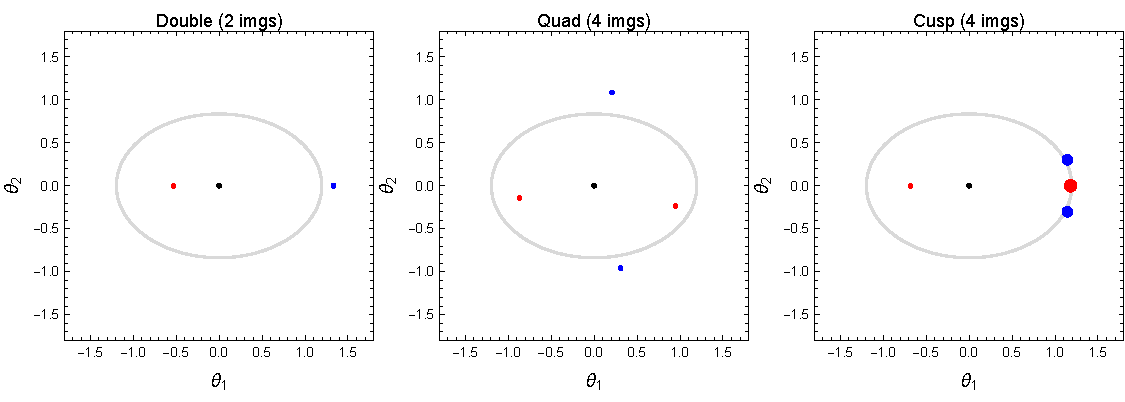
\includegraphics[width=0.95\textwidth]{../Figures/08_Elliptical_Models_Caustics/image_configurations.pdf}
    \caption{Image configurations for an SIE lens with
    $\thetaE = 1''$ and $q = 0.7$.  \textbf{Left:} Double (source
    outside caustic).  \textbf{Center:} Quad / Einstein cross
    (source inside caustic).  \textbf{Right:} Cusp configuration
    (source near a cusp).  Blue = Type~I (positive parity);
    red = Type~II (negative parity).  The critical curve and
    caustic are shown as gray curves.
    Generated by \texttt{critical\_curves\_caustics.wl}.}
    \label{fig:image_configs}
\end{figure}


% =====================================================================
\section{Summary}
\label{sec:elliptical_summary}

\begin{itemize}
    \item \textbf{SIS + external shear} is the simplest
          non-axisymmetric model.  The external shear
          $\gamma_{\mathrm{ext}}$ deforms the critical curve into an
          ellipse and opens the point caustic into a
          \textbf{diamond (astroid)} with four cusps.

    \item The \textbf{singular isothermal ellipsoid} (SIE) builds
          ellipticity directly into the mass distribution.  Its
          deflection angle involves $\arctan$ and $\mathrm{arctanh}$
          functions (Kormann et al.\ 1994).  It is the standard model
          for galaxy-scale lens modeling.

    \item \textbf{Critical curves} ($\det\Amat = 0$) are parity
          boundaries in the image plane.  The tangential critical
          curve ($1 - \kappab = |\gammaL|$) is the site of giant arcs;
          the radial critical curve ($1 - \kappab = -|\gammaL|$) is
          the site of radial arcs.

    \item \textbf{Caustics} are the mappings of critical curves to
          the source plane.  They divide the source plane into regions
          of different image multiplicity.

    \item \textbf{Image topology:}  As a source crosses a caustic,
          two images appear or disappear on opposite sides of the
          critical curve, with opposite parities.  This preserves
          Burke's odd-number theorem.

    \item \textbf{Fold caustics:}  Two images merge; magnification
          $|\mu| \propto 1/\sqrt{d_\perp}$.  This produces giant
          arcs.

    \item \textbf{Cusp caustics:}  Three images merge; the cusp
          relation $\mu_A + \mu_B + \mu_C \approx 0$ holds.

    \item \textbf{Image configurations:}  Doubles (source outside
          caustic), quads/Einstein crosses (source inside caustic),
          and cusp triplets (source near a cusp) account for the
          observed morphologies of strong lens systems.

    \item \textbf{Giant arcs} form when extended sources lie near the
          tangential caustic: images are tangentially stretched by
          factors of $\mu_{\mathrm{tan}} \propto 1/\sqrt{d_\perp}$
          along the tangential critical curve.
\end{itemize}


% =====================================================================
\section{Problems}
\label{sec:elliptical_problems}

\begin{exercise}
\label{ex:sis_shear_crit}
\textbf{(SIS + shear: critical curves and caustics.)}
Consider an SIS + external shear model with $\thetaE = 1''$ and
$\gamma_{\mathrm{ext}} = 0.1$.
\begin{enumerate}[label=(\alph*)]
    \item Starting from the lensing potential
          (eq.~\ref{eq:psi_sis_shear}), compute the Jacobian matrix
          $\Amat$ and the determinant $\det\Amat$ as functions of
          $(\theta_1, \theta_2)$.
    \item Solve $\det\Amat = 0$ to find the critical curve.  Express
          the result in polar coordinates $\theta_{\mathrm{crit}}(\phi)$.
          Plot the critical curve.
    \item Map the critical curve through the lens equation to obtain
          the caustic.  Plot the caustic in the source plane.  Verify
          that it has four cusps and the shape of an astroid.
    \item Estimate the area enclosed by the caustic (the quad
          cross-section).
\end{enumerate}
Verify with
\solnlink{08_Elliptical_Models_Caustics/problems\_08.wl}{problems\_08.wl}.
\end{exercise}

\begin{exercise}
\label{ex:sie_caustic}
\textbf{(SIE tangential caustic.)}
For an SIE with $\thetaE = 1''$ and axis ratio $q = 0.7$:
\begin{enumerate}[label=(\alph*)]
    \item Write down the deflection angle components $\alpha_1$ and
          $\alpha_2$ from eqs.~\eqref{eq:sie_alpha1}--\eqref{eq:sie_alpha2}.
    \item Compute the tangential caustic numerically by: (i)~finding
          the critical curve from $\det\Amat = 0$, and (ii)~mapping
          it through the lens equation.  Plot the caustic.
    \item Compute the area of the tangential caustic (the quad
          cross-section) numerically.  How does it compare to the
          SIS + shear model with the same effective ellipticity?
\end{enumerate}
Verify with
\solnlink{08_Elliptical_Models_Caustics/problems\_08.wl}{problems\_08.wl}.
\end{exercise}

\begin{exercise}
\label{ex:fold_magnification}
\textbf{(Fold magnification scaling.)}
Show that images appear or disappear in pairs at caustic crossings
by analyzing $\det\Amat$ near a fold:
\begin{enumerate}[label=(\alph*)]
    \item Near a fold caustic, the lens mapping in the direction
          perpendicular to the fold can be approximated as
          $\beta_\perp \approx a\,\theta_\perp^2$, where
          $\theta_\perp$ is the signed distance from the critical
          curve and $a$ is a constant.  Show that for
          $\beta_\perp > 0$, there are two solutions
          $\theta_\perp = \pm\sqrt{\beta_\perp/a}$ (one on each
          side of the critical curve), while for $\beta_\perp < 0$
          there are no solutions.
    \item Compute the Jacobian of the simplified mapping and show
          that the magnification scales as
          $|\mu| \propto 1/\sqrt{\beta_\perp}$ for each image.
    \item Show that the two images have opposite parities
          (opposite signs of $\det\Amat$).
\end{enumerate}
Verify with
\solnlink{08_Elliptical_Models_Caustics/problems\_08.wl}{problems\_08.wl}.
\end{exercise}

\begin{exercise}
\label{ex:sie_images}
\textbf{(SIE image positions.)}
For a source at $\vecbeta = (0.1, 0.2)''$ lensed by an SIE with
$\thetaE = 1''$ and $q = 0.8$:
\begin{enumerate}[label=(\alph*)]
    \item Determine whether the source is inside or outside the
          tangential caustic.  How many images do you expect?
    \item Find all image positions $\vectheta_i$ numerically by
          solving the lens equation
          $\vecbeta = \vectheta - \vecalpha(\vectheta)$.
    \item For each image, compute the magnification $\mu_i$ and
          determine the parity (Type~I or Type~II).
    \item Compute the signed magnification sum $\sum_i \mu_i$ and
          discuss whether it is consistent with the expected value
          (considering the missing central image for the singular SIE).
\end{enumerate}
Verify with
\solnlink{08_Elliptical_Models_Caustics/problems\_08.wl}{problems\_08.wl}.
\end{exercise}

\begin{exercise}
\label{ex:burke_verification}
\textbf{(Burke's odd-number theorem for the SIE.)}
Verify Burke's odd-number theorem for an SIE with $\thetaE = 1''$
and $q = 0.7$:
\begin{enumerate}[label=(\alph*)]
    \item For a source outside the tangential caustic (e.g.,
          $\vecbeta = (0.5, 0.0)''$), find all image positions.
          Count the images (including any faint central image) and
          verify the count is odd.
    \item For a source inside the tangential caustic (e.g.,
          $\vecbeta = (0.05, 0.05)''$), find all image positions.
          Verify the count is odd.
    \item For each case, classify each image by parity and verify
          that the number of positive-parity images exceeds the
          number of negative-parity images by one.
    \item Discuss why the SIE (being singular at the origin)
          requires care in applying Burke's theorem.  What role does
          the central image play?
\end{enumerate}
Verify with
\solnlink{08_Elliptical_Models_Caustics/problems\_08.wl}{problems\_08.wl}.
\end{exercise}

% =============================================================================
% Module 9: Strong Lensing by Galaxies: Applications
% =============================================================================
% Sources: Congdon & Keeton Ch. 6.5-6.6, Narayan & Bartelmann Sec. 3.6-3.7,
%          Saha et al.
% Mathematica: ../Mathematica/09_Galaxy_Lensing_Applications/
% =============================================================================

\chapter{Strong Lensing by Galaxies: Applications}
\label{ch:galaxy_lensing_applications}

% TODO: Module content to be written
% Topics:
% - Lens modeling and parameter estimation
% - Mass determination from lensing observables
% - Dark matter substructure
% - Flux ratio anomalies
% - H0 measurement from time delay cosmography

% =============================================================================
% Module 10: Strong Lensing by Galaxy Clusters
% =============================================================================
% Sources: Congdon & Keeton Ch. 7, Narayan & Bartelmann Sec. 4,
%          Meneghetti 2021 Ch. 5
% Mathematica: ../Mathematica/10_Cluster_Lensing/
% =============================================================================

\chapter{Strong Lensing by Galaxy Clusters}
\label{ch:cluster_lensing}

\begin{quote}
\textit{Galaxy clusters are the most massive gravitationally bound objects
in the universe.  When they act as gravitational lenses, they produce the
most dramatic manifestations of general relativity visible in the sky:
giant luminous arcs stretching tens of arcseconds, dozens of multiply
imaged background galaxies, and magnification factors large enough to
reveal individual stars at cosmological distances.}
\hfill --- adapted from Meneghetti (2021)
\end{quote}

\noindent
This final module brings together the entire gravitational lensing
framework developed in Modules~1--9 and applies it to the most
spectacular setting: \textbf{galaxy clusters}.  Where a single galaxy
lens (Module~9) typically produces two or four images of a background
source with an Einstein radius of $\sim 1''$, a massive galaxy cluster
can produce dozens of multiple image systems, giant arcs with
length-to-width ratios exceeding 10:1, and Einstein radii of
$\sim 10''$--$50''$.

Galaxy clusters have total masses of $10^{14}$--$10^{15}\,\Msun$,
with $\sim 85\%$ in dark matter, $\sim 13\%$ in hot intracluster gas,
and only $\sim 2\%$ in stars.  Their mass distributions are
well-described by the NFW profile introduced in
Module~\ref{ch:axisymmetric_models}, now applied at scales 100--1000
times more massive than individual galaxy halos.  The richness of
cluster lensing --- many image systems at multiple source redshifts ---
provides powerful constraints on the dark matter distribution and on
cosmological parameters.

\medskip
\noindent
\textbf{Companion Mathematica files:}
\begin{itemize}[nosep]
    \item \mathlink{10_Cluster_Lensing/cluster\_lensing.wl}{cluster\_lensing.wl}
          --- NFW cluster lensing quantities; critical curves and
          caustics at cluster scale; ray-tracing through cluster
          potential to generate arcs; Einstein radius vs.\ cluster mass;
          figures exported to \texttt{Figures/10\_Cluster\_Lensing/}
    \item \mathlink{10_Cluster_Lensing/nfw\_cluster.nb}{nfw\_cluster.nb}
          --- interactive notebook with \texttt{Manipulate} widgets for
          NFW cluster parameters, giant arc formation, magnification
          maps, and weak lensing shear profiles
\end{itemize}


% =====================================================================
\section{Introduction: Why Cluster Lensing Is Special}
\label{sec:cluster_intro}

Galaxy clusters occupy a unique place in both astrophysics and
gravitational lensing.  They are the largest objects in the universe
whose properties are determined by gravity alone --- they sit at the
top of the hierarchy of cosmic structure.  Their enormous masses make
them the most powerful gravitational lenses, producing phenomena that
are qualitatively different from galaxy-scale lensing:

\begin{enumerate}
    \item \textbf{Giant arcs.}  Extended background galaxies are
          stretched into luminous arcs tens of arcseconds long, tracing
          out the tangential critical curve of the cluster potential.
          The first giant arc was discovered in Abell~370 by Soucail
          et al.\ (1987), confirming the gravitational lensing
          interpretation of these features.

    \item \textbf{Many multiple image systems.}  A single massive
          cluster can produce 10--30 or more distinct sets of multiple
          images, each from a different background galaxy at a different
          redshift.  Each set independently constrains the cluster mass
          model.

    \item \textbf{Extreme magnification.}  Magnification factors of
          $\mu \sim 10$--100 are common near the critical curves of
          clusters.  This turns clusters into ``gravitational
          telescopes'' that reveal galaxies and even individual stars
          at redshifts $z > 6$ that would otherwise be undetectable.

    \item \textbf{Sensitivity to dark matter.}  Because clusters are
          dark-matter dominated, their lensing signal directly probes
          the dark matter distribution --- its radial profile,
          substructure, and overall mass.

    \item \textbf{Cosmological probe.}  The abundance and properties
          of cluster lenses depend on cosmological parameters
          ($\Omegam$, $\sigma_8$, the dark energy equation of state),
          making cluster lensing a tool for precision cosmology.
\end{enumerate}


% =====================================================================
\section{NFW Model for Cluster Lensing}
\label{sec:nfw_cluster}

In Module~\ref{ch:axisymmetric_models} (Section~\ref{sec:nfw}) we
introduced the NFW density profile as the universal dark matter halo
profile.  Here we apply it at \textbf{cluster scale}, where the
relevant parameters are much larger than for galaxy halos.

\subsection{Cluster-Scale NFW Parameters}

The NFW profile (eq.~\ref{eq:nfw_rho}) is parametrized by the virial
mass $M_{200}$ and concentration $c = r_{200}/r_s$.  Typical values
for galaxy clusters are:
\begin{center}
\begin{tabular}{lcc}
\toprule
\textbf{Parameter} & \textbf{Galaxy halo} & \textbf{Cluster halo} \\
\midrule
$M_{200}$ & $10^{12}\,\Msun$ & $10^{14}$--$10^{15}\,\Msun$ \\
$c$ & $10$--$20$ & $3$--$8$ \\
$r_s$ & $15$--$30$ kpc & $200$--$500$ kpc \\
$r_{200}$ & $200$--$300$ kpc & $1$--$2$ Mpc \\
\bottomrule
\end{tabular}
\end{center}
The key difference is that clusters are \textit{less concentrated}
($c \sim 3$--$8$) than galaxy halos ($c \sim 10$--$20$), reflecting
their later formation epoch in the hierarchical structure formation
scenario.  Despite the lower concentration, the vastly greater mass
more than compensates, producing far stronger lensing.

\subsection{Lensing Quantities at Cluster Scale}

The NFW convergence, deflection angle, and shear from
Module~\ref{ch:axisymmetric_models} (eqs.~\ref{eq:nfw_kappa}--\ref{eq:nfw_gamma})
apply directly.  We collect the key formulae here for reference.  Define
$x = \theta/\theta_s$, where $\theta_s = r_s/\Dd$ is the angular scale
radius.  Then:
\begin{align}
    \kappab(x) &= \kappa_s\, f(x) \,,
    \label{eq:cl_nfw_kappa} \\
    \alpha(x) &= \frac{4\kappa_s\,\theta_s}{x}
    \left[\ln\frac{x}{2} + g(x)\right] \,,
    \label{eq:cl_nfw_alpha} \\
    |\gammaL(x)| &= \bar{\kappa}(x) - \kappab(x) \,,
    \label{eq:cl_nfw_gamma}
\end{align}
with the functions $f(x)$ and $g(x)$ defined in
eqs.~\eqref{eq:nfw_f}--\eqref{eq:nfw_g}, and the characteristic
convergence:
\begin{equation}
    \kappa_s = \frac{2\rho_s\, r_s}{\Sigmacr} \,.
    \label{eq:cl_kappa_s}
\end{equation}

\begin{example}
\textbf{Characteristic convergence for a massive cluster.}
For a cluster with $M_{200} = 10^{15}\,\Msun$, $c = 5$, at
$z_d = 0.3$ lensing a source at $z_s = 2$
($\Dd \approx 900$~Mpc, $\Ds \approx 1750$~Mpc,
$\Dds \approx 1400$~Mpc):
\begin{itemize}[nosep]
    \item $r_{200} \approx 2.0$~Mpc, $r_s = r_{200}/c \approx 400$~kpc,
    \item $\theta_s = r_s / \Dd \approx 92''$,
    \item $\kappa_s \approx 0.46$.
\end{itemize}
Since $\kappa_s \times f(x)$ can exceed unity for $x \lesssim 0.5$
(i.e., $\theta \lesssim 46''$), the cluster is a strong lens ---
it has a region where $\kappab > 1$.  These values are computed and
verified in
\mathlink{10_Cluster_Lensing/cluster\_lensing.wl}{cluster\_lensing.wl}.
\end{example}

\subsection{Critical Curves and Caustics for Cluster NFW}
\label{sec:cluster_crit}

For the circularly symmetric NFW profile, the tangential and radial
critical curves are circles.  The tangential critical curve occurs
where $\bar{\kappa}(x) = 1$, i.e.:
\begin{equation}
    \frac{4\kappa_s}{x_t^2}\left[\ln\frac{x_t}{2} + g(x_t)\right] = 1 \,,
    \label{eq:cl_tangential_crit}
\end{equation}
and the radial critical curve where
$2\kappab(x_r) - \bar{\kappa}(x_r) = 1$, i.e.:
\begin{equation}
    2\kappa_s\, f(x_r)
    - \frac{4\kappa_s}{x_r^2}\left[\ln\frac{x_r}{2} + g(x_r)\right] = 1 \,.
    \label{eq:cl_radial_crit}
\end{equation}
Both equations must be solved numerically.  For the cluster parameters
above ($M_{200} = 10^{15}\,\Msun$, $c = 5$, $z_d = 0.3$, $z_s = 2$),
the tangential critical curve has a radius of
$\theta_t \approx 35''$--$40''$, which corresponds to a physical
radius of $\sim 150$~kpc at the cluster redshift.

\begin{remark}
The tangential critical curve radius is often called the
\textbf{Einstein radius} of the cluster, $\thetaE$.  For a cluster,
$\thetaE \sim 10''$--$50''$, compared to $\sim 1''$ for a galaxy
lens.  The enclosed projected mass within $\thetaE$ is of order
$10^{13}$--$10^{14}\,\Msun$ --- the mass of a large galaxy group.
\end{remark}

\subsection{Einstein Radius Scaling with Cluster Mass}

The Einstein radius of an NFW cluster depends on mass, concentration,
and the lens/source redshift configuration.  For a fixed concentration
and redshift configuration, the scaling is approximately:
\begin{equation}
    \thetaE \propto M_{200}^{1/3} \,,
    \label{eq:cl_thetaE_scaling}
\end{equation}
which arises because $\thetaE \sim r_{200}/\Dd$ and
$r_{200} \propto M_{200}^{1/3}$ (from the definition
$M_{200} = (4\pi/3)\, 200\,\rho_{\mathrm{crit}}\, r_{200}^3$).
The actual relationship is more complex due to the dependence of
$\kappa_s$ on $c$ and the nonlinear solution of
eq.~\eqref{eq:cl_tangential_crit}, but the cube-root scaling provides
a useful approximation.

\begin{figure}[ht]
    \centering
    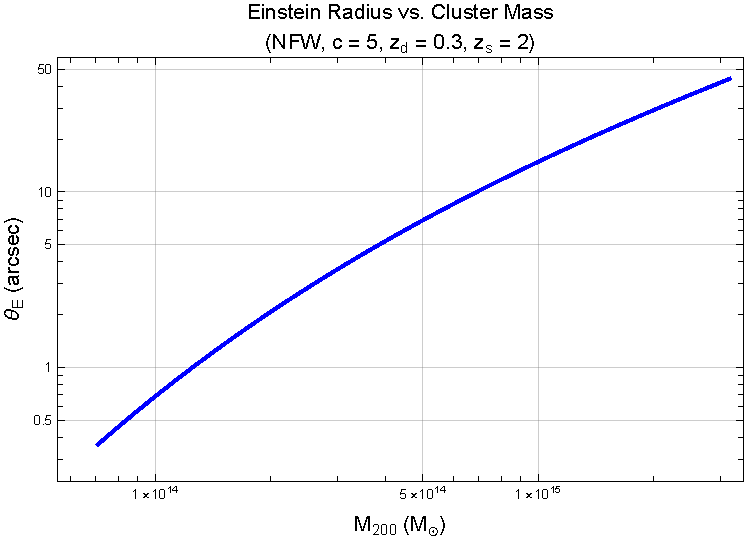
\includegraphics[width=0.75\textwidth]{../Figures/10_Cluster_Lensing/einstein_radius_vs_mass.pdf}
    \caption{Einstein radius $\thetaE$ as a function of cluster mass
    $M_{200}$ for an NFW profile with $c = 5$, $z_d = 0.3$, and
    $z_s = 2$.  The dashed line shows the approximate $M^{1/3}$
    scaling.  Clusters below $M_{200} \sim 10^{14}\,\Msun$ have
    Einstein radii comparable to galaxy-scale lenses.  Generated by
    \texttt{cluster\_lensing.wl}.}
    \label{fig:einstein_radius_vs_mass}
\end{figure}


% =====================================================================
\section{Giant Arcs}
\label{sec:giant_arcs}

Giant luminous arcs are the most visually striking signature of cluster
strong lensing.  They were first discovered by Lynds \& Petrosian (1986)
and Soucail et al.\ (1987) in the clusters Abell~370 and Cl~2244-02,
and their interpretation as gravitationally lensed images of background
galaxies was confirmed spectroscopically by Soucail et al.\ (1988).

\subsection{Formation Mechanism}

Giant arcs form when an extended background galaxy lies close to the
\textbf{tangential caustic} of the cluster.  From the theory of
critical curves (Module~\ref{ch:elliptical_models},
Section~\ref{sec:giant_arcs}):
\begin{enumerate}
    \item The source galaxy is near (but not exactly on) the tangential
          caustic in the source plane.
    \item Its images lie near the tangential critical curve in the image
          plane, where $\lambda_- \approx 0$.
    \item The images are stretched \textit{tangentially} (along the
          critical curve) by a large factor
          $\mu_{\mathrm{tan}} \propto 1/\sqrt{d_\perp}$, where
          $d_\perp$ is the perpendicular distance from the caustic.
    \item The radial magnification remains of order unity, so the
          image is a thin, elongated \textbf{arc} that traces the
          critical curve.
\end{enumerate}

\subsection{Ray-Tracing Through a Cluster Potential}
\label{sec:ray_trace}

To visualize arc formation, we \textbf{ray-trace} an extended source
through the cluster lens equation.  The procedure is:
\begin{enumerate}
    \item Define the source as a set of points in the source plane,
          e.g., a circular disk of angular radius $\beta_0$ centered
          at position $\vecbeta_0$.
    \item For each source point $\vecbeta$, solve the lens equation
          $\vecbeta = \vectheta - \vecalpha(\vectheta)$ for all
          image positions $\vectheta$.  For a cluster, this is done
          numerically on a fine grid.
    \item Plot the union of all image positions to obtain the lensed
          image of the source.
\end{enumerate}

In practice, it is more efficient to use the \textbf{inverse
ray-tracing} approach: for each pixel $\vectheta$ in the image
plane, compute $\vecbeta = \vectheta - \vecalpha(\vectheta)$ and
check whether $\vecbeta$ falls within the source.  If it does,
that pixel is part of a lensed image.

\begin{figure}[ht]
    \centering
    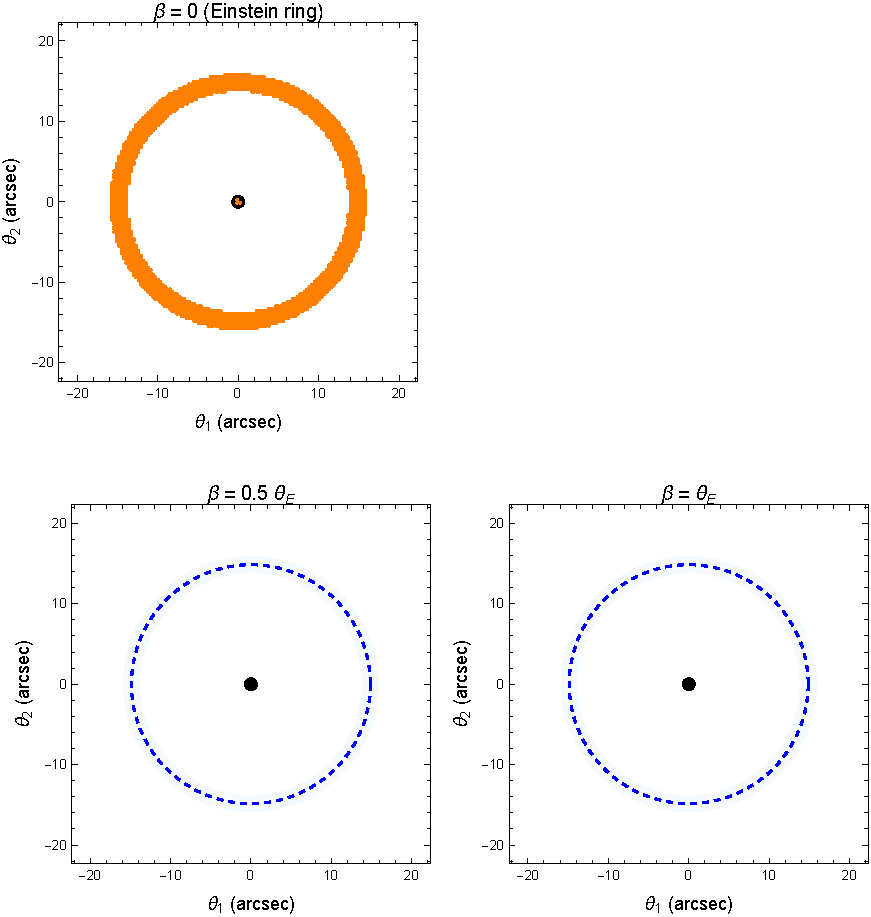
\includegraphics[width=0.85\textwidth]{../Figures/10_Cluster_Lensing/giant_arc_formation.pdf}
    \caption{Giant arc formation by an NFW cluster
    ($M_{200} = 10^{15}\,\Msun$, $c = 5$, $z_d = 0.3$, $z_s = 2$).
    A circular source of radius $0.5''$ is placed at three positions:
    $\beta = 0$ (Einstein ring, left), $\beta = 0.5\,\thetaE$
    (giant arc, center), and $\beta = \thetaE$ (near the critical
    curve, right).  The critical curve is shown as a dashed circle.
    Generated by \texttt{cluster\_lensing.wl}.}
    \label{fig:giant_arc_formation}
\end{figure}

\subsection{Length-to-Width Ratio}

The \textbf{length-to-width ratio} (or axis ratio) of an arc is a
direct measure of the tangential magnification:
\begin{equation}
    \frac{L}{W} \approx \mu_{\mathrm{tan}}
    = \frac{1}{|1 - \bar{\kappa}(\theta)|}
    \propto \frac{1}{\sqrt{d_\perp}} \,,
    \label{eq:arc_lw_ratio}
\end{equation}
where $L$ and $W$ are the length and width of the arc.  Observationally,
arcs with $L/W \geq 10$ are classified as ``giant arcs'', while those
with $3 \leq L/W < 10$ are often called ``arclets''.

\subsection{Arc Statistics}
\label{sec:arc_statistics}

The probability that a cluster produces a giant arc depends on:
\begin{itemize}
    \item \textbf{Cluster mass:} More massive clusters have larger
          Einstein radii and larger tangential caustics, increasing the
          cross-section for arc production.  The arc cross-section
          scales steeply with mass, roughly as $\sigma_{\mathrm{arc}}
          \propto M_{200}^{2\text{--}3}$.
    \item \textbf{Source redshift:} Higher source redshifts increase
          $\Dds/\Ds$, which increases $\kappa_s$ and the Einstein
          radius.
    \item \textbf{Cluster ellipticity and substructure:}
          Non-axisymmetric mass distributions and merging clusters
          enhance the arc cross-section significantly, often by a
          factor of 2--5.
    \item \textbf{Source size and morphology:} Extended sources are
          more easily stretched into arcs; compact sources are more
          likely to appear as multiple point-like images.
\end{itemize}

\begin{remark}
Arc statistics have been a source of tension with cosmological models.
Bartelmann et al.\ (1998) found that the observed number of giant arcs
exceeded the prediction from $\Lambda$CDM by a factor of $\sim$10.
This ``arc statistics problem'' has been partially resolved by
accounting for cluster ellipticity, substructure, and the contribution
of baryonic physics (cooling, AGN feedback) to the central mass
concentration, but it remains an active area of research.
\end{remark}


% =====================================================================
\section{Multiple Image Systems in Clusters}
\label{sec:multiple_images}

One of the most powerful aspects of cluster lensing is that a single
cluster can lens \textbf{many} background galaxies simultaneously,
producing multiple sets of multiple images.  Each set of images
(called an ``image family'' or ``image system'') comes from a single
background source at a particular redshift.

\subsection{Image Families}

A typical strong lensing cluster produces:
\begin{itemize}
    \item \textbf{5--10 secure image families} with spectroscopic
          redshift confirmation in well-studied clusters.
    \item \textbf{20--50 candidate image families} identified by
          morphology, color, and photometric redshifts in deep imaging
          surveys.
    \item In extreme cases (e.g., Abell~1689), over 100 candidate
          images have been identified from more than 30 distinct
          background sources.
\end{itemize}

Each image family provides independent constraints on the cluster mass
model:
\begin{enumerate}
    \item The \textbf{image positions} constrain the deflection field
          $\vecalpha(\vectheta)$ at several points.
    \item The \textbf{magnification ratios} (flux ratios between images)
          constrain the convergence and shear fields.
    \item The \textbf{redshift} of each family provides a distance
          ratio $\Dds/\Ds$ that weights the lensing signal differently,
          breaking degeneracies in the mass model.
\end{enumerate}

\subsection{Spectroscopic Confirmation}

Image families are confirmed by matching the redshifts of candidate
images: if multiple images at different positions have the same
spectroscopic redshift, they are identified as images of the same
source.  Modern multi-object spectrographs (VLT/MUSE, Keck/DEIMOS)
have been transformative for cluster lensing, enabling redshift
measurements of faint, highly magnified background galaxies.

\subsection{Famous Cluster Lenses}

Several galaxy clusters have become benchmarks for strong lensing
studies:
\begin{itemize}
    \item \textbf{Abell~370} ($z = 0.375$): Site of the first
          discovered giant arc (Soucail et al.\ 1987).  Over 10
          multiple image systems identified.
    \item \textbf{Abell~1689} ($z = 0.183$): One of the most
          powerful known lenses, with over 100 images from $\sim$30
          background sources.  Its Einstein radius of $\sim 47''$
          (for $z_s \sim 2$) is among the largest known.
    \item \textbf{MACSJ0416.1-2403} ($z = 0.396$): A Hubble Frontier
          Field cluster with over 60 spectroscopically confirmed
          multiple images, used for detailed mass reconstruction.
    \item \textbf{Abell~2744} ($z = 0.308$): The ``Pandora's Cluster'',
          a complex merging system with extensive strong and weak
          lensing constraints.
\end{itemize}


% =====================================================================
\section{Cluster Mass Estimation}
\label{sec:mass_estimation}

Gravitational lensing provides a \textit{direct} measurement of the
projected mass distribution of a cluster, independent of assumptions
about the dynamical state of the system.  This makes it
complementary to X-ray and kinematic mass estimates, which rely on
assumptions of hydrostatic or virial equilibrium.

\subsection{Strong Lensing Mass Estimates}

Strong lensing constrains the mass distribution in the
\textbf{inner region} of the cluster, typically within
$\sim 200$--$300$~kpc of the center.  The basic approach is:
\begin{enumerate}
    \item \textbf{Identify multiple image systems} and measure their
          positions and redshifts.
    \item \textbf{Parametrize the mass model.}  The cluster mass is
          described by one or more NFW halos (for the smooth dark
          matter component) plus additional components for cluster
          member galaxies (typically scaled isothermal profiles).
    \item \textbf{Optimize the model parameters} by minimizing the
          difference between predicted and observed image positions.
          Modern codes (e.g., \texttt{lenstool}, \texttt{glafic})
          use Bayesian methods (MCMC) to explore the parameter space.
    \item \textbf{Derive the mass profile} from the best-fit model.
\end{enumerate}

A quick estimate of the enclosed mass within the Einstein radius is
provided by:
\begin{equation}
    \boxed{
    M(\theta \leq \thetaE) = \pi\, (\Dd\, \thetaE)^2\, \Sigmacr
    }
    \label{eq:mass_within_thetaE}
\end{equation}
since $\bar{\kappa}(\thetaE) = 1$ by definition.  For a cluster with
$\thetaE = 30''$ at $z_d = 0.3$ with $z_s = 2$:
\begin{equation}
    M(\thetaE) \approx 2 \times 10^{14}\,\Msun \,.
    \label{eq:mass_numerical}
\end{equation}
This is the projected mass within a cylinder of radius
$\sim 130$~kpc --- a substantial fraction of the total cluster mass.
The exact value is computed in
\mathlink{10_Cluster_Lensing/cluster\_lensing.wl}{cluster\_lensing.wl}.

\subsection{Weak Lensing Mass Estimates (Preview)}

Strong lensing probes only the inner $\sim$10\% of the cluster virial
radius.  To measure the total cluster mass, one must extend to larger
radii using \textbf{weak lensing} (Section~\ref{sec:weak_lensing}).

\subsection{Combining Strong and Weak Lensing}

The most accurate cluster mass profiles come from combining strong
and weak lensing:
\begin{itemize}
    \item \textbf{Strong lensing} provides high-resolution constraints
          on the inner mass profile ($r \lesssim 200$~kpc), including
          the NFW concentration parameter.
    \item \textbf{Weak lensing} provides constraints at larger radii
          ($200$~kpc $\lesssim r \lesssim 3$~Mpc), determining the
          virial mass $M_{200}$.
    \item The combined profile spans nearly two decades in radius and
          is well-fit by an NFW profile, supporting the universality
          of the dark matter halo profile.
\end{itemize}

\subsection{Comparison with Other Mass Estimators}

Cluster masses can also be estimated from:
\begin{itemize}
    \item \textbf{X-ray observations:} The hot intracluster medium
          (ICM) emits thermal bremsstrahlung X-rays.  Under the
          assumption of hydrostatic equilibrium, the gas temperature
          and density profiles yield the total mass profile.
          Hydrostatic masses are typically 10--20\% lower than lensing
          masses (the ``hydrostatic mass bias''), likely due to
          non-thermal pressure support from turbulence and bulk motions.
    \item \textbf{Galaxy velocity dispersion:} The velocities of
          cluster member galaxies, combined with the virial theorem,
          yield a mass estimate.  This method is noisy (requiring many
          galaxy redshifts) and sensitive to interlopers.
    \item \textbf{Sunyaev--Zel'dovich (SZ) effect:} Inverse Compton
          scattering of CMB photons by the hot ICM produces a spectral
          distortion.  The integrated SZ signal is proportional to the
          total thermal energy and correlates with total mass.
\end{itemize}

\begin{remark}
The complementarity of these methods is powerful.  Comparing lensing
masses (which are model-independent) with X-ray/SZ masses (which
assume hydrostatic equilibrium) calibrates the hydrostatic mass bias,
which is a critical systematic in using cluster counts for cosmology.
\end{remark}


% =====================================================================
\section{Magnification and the Cosmic Telescope}
\label{sec:cosmic_telescope}

Perhaps the most exciting application of cluster lensing in
contemporary astrophysics is the use of massive clusters as
\textbf{gravitational telescopes}: natural magnifying glasses that
amplify the light of distant background galaxies, allowing us to
study objects that would otherwise be far too faint to detect.

\subsection{Magnification by Clusters}

Near the critical curves of a massive cluster, the magnification can
reach $\mu \sim 10$--$100$ or more.  Since the observed flux scales as
$\mu$ (for sources smaller than the scale over which $\mu$ varies),
a source at $z \sim 10$ behind a cluster lens can appear as bright as
an unmagnified source at $z \sim 3$--$4$.

The trade-off is that magnification also reduces the effective area
in the source plane.  A magnification of $\mu$ enlarges the image
area by $\mu$ but surveys a source-plane area that is $\mu$ times
smaller.  The net effect on the number of detected sources depends on
the slope of the luminosity function --- this is the
\textbf{magnification bias}.

\subsection{Magnification Bias}

The magnification bias arises because lensing simultaneously:
\begin{enumerate}
    \item \textbf{Amplifies flux:} Sources below the detection
          threshold are boosted above it, increasing the detected
          number.
    \item \textbf{Dilutes area:} The effective survey area is reduced
          by $1/\mu$, decreasing the detected number.
\end{enumerate}
For a cumulative luminosity function $N(>S) \propto S^{-\alpha}$
(where $S$ is flux and $\alpha$ is the faint-end slope), the net
number count behind a lens changes by a factor of
$\mu^{\alpha - 1}$.  For $\alpha > 1$ (steep luminosity function),
magnification bias \textit{increases} the number of detected sources;
for $\alpha < 1$, it \textit{decreases} the count.  At high
redshift, the luminosity function is steep ($\alpha \gtrsim 2$), so
there is a significant net increase in detected galaxies behind
clusters.

\subsection{The Hubble Frontier Fields}

The Hubble Frontier Fields (HFF) program (2013--2017) was a major
HST initiative that obtained ultra-deep imaging of six massive
galaxy clusters chosen for their strong lensing power:
\begin{enumerate}[nosep]
    \item Abell~2744 ($z = 0.308$)
    \item MACSJ0416.1-2403 ($z = 0.396$)
    \item MACSJ0717.5+3745 ($z = 0.545$)
    \item MACSJ1149.5+2223 ($z = 0.543$)
    \item Abell~S1063 ($z = 0.348$)
    \item Abell~370 ($z = 0.375$)
\end{enumerate}
These clusters were used as gravitational telescopes to detect
galaxies at $z \sim 6$--$10$, probing the epoch of reionization.
The HFF program discovered some of the most distant galaxies known
at the time and provided detailed mass models of the six clusters
from their many multiple image systems.

\subsection{JWST and the New Era of Cluster Lensing}

The James Webb Space Telescope (JWST, launched 2021) has
revolutionized cluster lensing with its superior infrared sensitivity
and angular resolution.  Notable results include:
\begin{itemize}
    \item \textbf{Earendel} (WHL0137-LS): The most distant individual
          star known, at $z = 6.2$, magnified by a factor of
          $\mu \gtrsim 4000$ by the cluster WHL~0137-08
          (Welch et al.\ 2022).  The extreme magnification occurs
          because the star lies almost exactly on the cluster's
          critical curve.
    \item \textbf{The Sunrise Arc}: A galaxy at $z = 6.2$ lensed into
          a long arc by the same cluster, in which Earendel was
          identified as a point source on the arc.
    \item \textbf{Early galaxy candidates at $z > 10$}: Lensed
          galaxies behind clusters observed with JWST/NIRCam have
          pushed the redshift frontier beyond $z \sim 13$, with
          magnifications of $\mu \sim 5$--$30$ making these detections
          possible.
\end{itemize}

\begin{remark}
The discovery of Earendel illustrates the extreme power of cluster
lensing.  An individual star at $z = 6.2$ has an apparent magnitude
of $m \sim 40$ without magnification --- utterly undetectable.  A
magnification of $\mu \sim 4000$ corresponds to $\Delta m \sim -9$
magnitudes, bringing it within reach of HST and JWST\@.  However,
such extreme magnification requires the source to be within
$\sim 0.001''$ of the critical curve, making such discoveries
exceedingly rare.
\end{remark}


% =====================================================================
\section{Brief Introduction to Weak Lensing}
\label{sec:weak_lensing}

Throughout Modules~1--9 and the preceding sections of this module,
we have focused on \textbf{strong lensing}: the regime where
$\kappab \gtrsim 1$ and multiple images or giant arcs are produced.
But gravitational lensing does not stop at the strong lensing regime.
At larger radii from the cluster center (and behind foreground mass
distributions in general), the lensing effect is weak --- too small
to produce multiple images, but still measurable statistically.  This
is the domain of \textbf{weak gravitational lensing}.

This section provides a brief introduction to weak lensing --- just
enough to show where the field goes beyond strong lensing and to
connect to the rich literature on the subject.  A full treatment of
weak lensing is beyond the scope of these tutorials.

\subsection{The Weak Lensing Regime}

In the weak lensing regime, $\kappab \ll 1$ and $|\gammaL| \ll 1$.
There are no multiple images or giant arcs.  Instead, the primary
observable effect is a small, coherent \textbf{distortion} (shearing)
of the shapes of background galaxies.  An intrinsically circular
galaxy is sheared into a slightly elliptical shape, with the
orientation and magnitude of the induced ellipticity determined by the
local shear field.

The key challenge is that individual galaxy shapes are intrinsically
elliptical, with typical intrinsic ellipticities of
$|\epsilon_{\mathrm{int}}| \sim 0.2$--$0.3$.  The gravitational
shear signal is $|\gammaL| \sim 0.01$--$0.05$ in the weak lensing
regime --- much smaller than the intrinsic shape noise.  Therefore,
one must \textbf{average} over many background galaxies to extract
the coherent shear signal.

\subsection{The Reduced Shear}

In the weak lensing regime, the observable quantity is the
\textbf{reduced shear}:
\begin{equation}
    \boxed{
    g = \frac{\gammaL}{1 - \kappab}
    }
    \label{eq:reduced_shear}
\end{equation}
This is because the lensing transformation preserves surface
brightness, and the observed ellipticity of a lensed galaxy (for
$|g| \leq 1$) is:
\begin{equation}
    \epsilon^{\mathrm{obs}} = \frac{\epsilon^{\mathrm{int}} + g}
    {1 + g^*\, \epsilon^{\mathrm{int}}}
    \approx \epsilon^{\mathrm{int}} + g \,,
    \label{eq:observed_ellipticity}
\end{equation}
where the approximation holds for $|g| \ll 1$.  Since intrinsic
ellipticities are randomly oriented (in the absence of intrinsic
alignments), their average vanishes:
$\langle\epsilon^{\mathrm{int}}\rangle \approx 0$.  Therefore:
\begin{equation}
    \langle \epsilon^{\mathrm{obs}} \rangle \approx g
    \approx \gammaL \quad (\text{for } \kappab \ll 1) \,.
    \label{eq:shear_estimator}
\end{equation}
The mean observed ellipticity of background galaxies is an unbiased
estimator of the shear (in the weak limit).

\subsection{Tangential Shear Profile Around Clusters}

For a circularly symmetric mass distribution, the shear is purely
tangential.  The \textbf{tangential shear} at angular distance
$\theta$ from the cluster center is:
\begin{equation}
    \gamma_t(\theta) = \bar{\kappa}(\theta) - \kappab(\theta) \,,
    \label{eq:tangential_shear}
\end{equation}
which we recognize from eq.~\eqref{eq:gamma_circular}
(Module~\ref{ch:axisymmetric_models}).  The tangential shear profile
$\gamma_t(\theta)$ can be measured by averaging the tangential
component of the ellipticities of background galaxies in annular
bins around the cluster center.

For an NFW profile, $\gamma_t(\theta)$ has a characteristic shape
that rises toward the center (reaching the strong lensing regime) and
falls off at large radii.  Fitting the observed $\gamma_t(\theta)$
profile to the NFW prediction yields the cluster mass $M_{200}$ and
concentration $c$.

\subsection{From Clusters to Cosmic Shear}

The weak lensing framework extends far beyond individual cluster
halos.  The \textbf{cosmic shear} signal --- the coherent shearing of
galaxy shapes by the entire large-scale structure of the universe
along the line of sight --- is one of the primary probes of modern
cosmology.  Cosmic shear measurements constrain the matter power
spectrum, the matter density $\Omegam$, and the amplitude of matter
fluctuations $\sigma_8$.

Current and upcoming surveys measuring cosmic shear include:
\begin{itemize}[nosep]
    \item \textbf{Euclid} (ESA, launched 2023): space-based imaging of
          $\sim$1.5 billion galaxies over 15{,}000~deg$^2$.
    \item \textbf{Vera C.~Rubin Observatory / LSST}: ground-based
          survey of $\sim$4 billion galaxies over 18{,}000~deg$^2$
          (first light expected 2025).
    \item \textbf{Nancy Grace Roman Space Telescope} (NASA, expected
          launch 2027): space-based survey complementing Euclid.
\end{itemize}

These surveys will measure cosmic shear with percent-level precision,
providing powerful constraints on dark energy, modified gravity, and
the neutrino mass hierarchy.


% =====================================================================
\section{The State of the Field and Future Directions}
\label{sec:future}

Strong lensing by galaxy clusters is a mature but rapidly evolving
field.  The combination of new observational facilities and
sophisticated modeling techniques continues to push the boundaries of
what cluster lensing can teach us.

\subsection{Current Observational Facilities}

\begin{itemize}
    \item \textbf{HST:} The Hubble Space Telescope has been the
          workhorse for cluster strong lensing for three decades, with
          programs like the Hubble Frontier Fields and RELICS
          (Reionization Lensing Cluster Survey) producing the deepest
          cluster lensing data.
    \item \textbf{JWST:} With its infrared capabilities, JWST is
          discovering lensed galaxies at $z > 10$, measuring
          spectroscopic redshifts of multiple image systems, and
          resolving detailed structure in giant arcs.
    \item \textbf{Euclid:} The wide-field survey will discover
          thousands of new cluster lenses, dramatically increasing the
          statistical power of cluster lensing studies.
    \item \textbf{Rubin/LSST:} The deep, wide survey will combine
          strong and weak lensing for a large sample of clusters, with
          time-domain capability for detecting lensed transients.
\end{itemize}

\subsection{Future Facilities}

\begin{itemize}
    \item \textbf{Nancy Grace Roman Space Telescope:} High-resolution,
          wide-field infrared imaging will complement JWST for cluster
          lensing studies.
    \item \textbf{Square Kilometre Array (SKA):} Radio weak lensing
          with the SKA will provide shape measurements free from many
          of the systematics that affect optical measurements
          (atmospheric seeing, PSF modeling).
    \item \textbf{Extremely Large Telescopes} (ELT, TMT, GMT):
          Ground-based 25--39m telescopes with adaptive optics will
          resolve sub-arcsecond structure in cluster arcs and obtain
          spectra of extremely faint lensed sources.
\end{itemize}

\subsection{Open Questions}

\begin{enumerate}
    \item \textbf{Dark matter substructure:} CDM predicts a rich
          hierarchy of subhalos within clusters.  The number and mass
          function of subhalos affect the lensing signal (flux ratio
          anomalies, perturbations to giant arcs).  Comparing
          predictions to observations constrains alternative dark
          matter models (warm dark matter, self-interacting dark
          matter).

    \item \textbf{The nature of dark matter:} The inner density
          profile of clusters (cusp vs.\ core) is sensitive to dark
          matter self-interactions.  Strong lensing at the center of
          clusters provides the highest-resolution probe of the dark
          matter profile.

    \item \textbf{The cluster mass function:} The abundance of massive
          clusters as a function of mass and redshift is a sensitive
          cosmological probe.  Lensing-calibrated cluster masses are
          essential for turning cluster counts into cosmological
          constraints.

    \item \textbf{Multi-plane lensing and line-of-sight effects:}
          Light rays from distant sources pass through multiple mass
          concentrations along the line of sight.  Accounting for
          these ``line-of-sight'' effects is important for precision
          mass modeling.

    \item \textbf{Time-delay cosmography with clusters:} Time delays
          between multiple images of time-varying sources (supernovae,
          quasars) in clusters constrain $\Hubble$.  The multiply
          imaged supernova ``Refsdal'' in MACSJ1149 (Kelly et al.\
          2015) was the first such measurement.
\end{enumerate}

\subsection{Connection to the AGEL Project}

The ASTRO 3D Galaxy Evolution with Lensing (AGEL) survey is a
spectroscopic survey of galaxy-scale strong lens candidates selected
from wide-field imaging surveys.  While AGEL focuses on galaxy-scale
lenses rather than clusters, many of the techniques and physical
principles are the same:
\begin{itemize}[nosep]
    \item NFW profiles and isothermal models describe the lens mass
          distribution at both galaxy and cluster scales.
    \item Critical curves and caustics determine the image
          configurations at all mass scales.
    \item Strong lensing mass estimates and comparisons with dynamical
          masses apply to both galaxy and cluster lenses.
\end{itemize}
The transition from galaxy to cluster lensing is one of scale rather
than fundamental physics --- the same equations derived in
Modules~1--9 govern both regimes.


% =====================================================================
\section{Summary}
\label{sec:cluster_summary}

\begin{itemize}
    \item \textbf{Galaxy clusters} ($M_{200} \sim 10^{14}$--$10^{15}\,
          \Msun$) are the most powerful gravitational lenses, producing
          giant arcs, dozens of multiple image systems, and
          magnification factors of $\mu \sim 10$--$100$.

    \item The \textbf{NFW profile} at cluster scale has
          $c \sim 3$--$8$ and $r_s \sim 200$--$500$~kpc.  The
          Einstein radius is $\thetaE \sim 10''$--$50''$, enclosing
          a projected mass of $\sim 10^{14}\,\Msun$.

    \item \textbf{Giant arcs} form when extended sources lie near the
          tangential caustic.  The length-to-width ratio
          $L/W \approx \mu_{\mathrm{tan}} \propto 1/\sqrt{d_\perp}$
          can exceed 10:1 for sources very close to the caustic.

    \item \textbf{Multiple image systems} (10--30+ per cluster) each
          independently constrain the mass model.  Spectroscopic
          confirmation via redshift matching identifies image families.

    \item \textbf{Cluster mass estimation} uses strong lensing (inner
          profile) and weak lensing (outer profile), complemented by
          X-ray and SZ measurements.  Strong lensing gives
          $M(\thetaE) = \pi(\Dd\,\thetaE)^2\,\Sigmacr$.

    \item Clusters serve as \textbf{gravitational telescopes},
          magnifying high-redshift galaxies and enabling discoveries
          like Earendel ($z = 6.2$, $\mu \gtrsim 4000$) and galaxies
          at $z > 10$.

    \item \textbf{Weak lensing} measures the statistical shear
          $\langle\epsilon\rangle \approx g = \gammaL/(1-\kappab)$ of
          background galaxies.  The tangential shear profile
          $\gamma_t(\theta)$ yields the cluster mass profile at large
          radii.

    \item \textbf{Current and future facilities} (JWST, Euclid,
          Rubin/LSST, Roman, SKA) will transform cluster lensing with
          larger samples, deeper imaging, and new wavelength regimes.
\end{itemize}

\subsection*{Where to Go from Here}

This module concludes the \textit{Learning to Lens} tutorial suite.
We have covered the foundations of general relativity
(Modules~1a--1e), the theory of gravitational lensing
(Modules~2--6), and the modeling and application of strong lensing
(Modules~7--10).  For readers who wish to continue deeper into the
field, we suggest the following directions:

\begin{itemize}
    \item \textbf{Advanced topics not covered in these tutorials:}
          dark matter substructure and flux ratio anomalies;
          line-of-sight effects and multi-plane lensing;
          free-form (non-parametric) mass reconstruction; lens
          modeling with extended source morphology; microlensing by
          stars in the lensing galaxy.

    \item \textbf{Software packages for lens modeling:}
          \begin{itemize}[nosep]
              \item \texttt{lenstronomy}
                    (\url{https://github.com/lenstronomy/lenstronomy}):
                    a comprehensive Python package for gravitational
                    lens modeling and simulation.
              \item \texttt{PyAutoLens}
                    (\url{https://github.com/Jammy2211/PyAutoLens}):
                    automated strong lens modeling with Bayesian
                    inference.
              \item \texttt{glafic}
                    (\url{https://www.slac.stanford.edu/~oguri/glafic/}):
                    a fast lens modeling code widely used for cluster
                    lensing.
              \item \texttt{GRALE}
                    (\url{https://research.edm.uhasselt.be/~jlieMDC/}):
                    free-form mass reconstruction using a genetic
                    algorithm.
          \end{itemize}

    \item \textbf{Key review articles for further reading:}
          Kneib \& Natarajan (2011), ``Cluster lenses'', A\&A Rev.;
          Treu (2010), ``Strong Lensing by Galaxies'', ARA\&A;
          Bartelmann \& Schneider (2001), ``Weak Gravitational
          Lensing'', Phys.\ Rep.;
          Kilbinger (2015), ``Cosmology with Cosmic Shear'',
          Rep.\ Prog.\ Phys.

    \item \textbf{Active research:} The AGEL project
          (Tran et al.\ 2022) exemplifies how the techniques developed
          in these tutorials are applied in practice.  Finding,
          confirming, and modeling galaxy-scale strong lenses in
          wide-field surveys is an active area of research to which
          the reader is now well-prepared to contribute.
\end{itemize}


% =====================================================================
\section{Problems}
\label{sec:cluster_problems}

\begin{exercise}
\label{ex:nfw_cluster_einstein}
\textbf{(NFW cluster Einstein radius and enclosed mass.)}
Consider an NFW cluster with $M_{200} = 5\ee{14}\,\Msun$, $c = 5$,
at $z_d = 0.3$ lensing a source at $z_s = 2$.  Use
$\Dd = 900$~Mpc, $\Ds = 1750$~Mpc, $\Dds = 1400$~Mpc.
\begin{enumerate}[label=(\alph*)]
    \item Compute the NFW parameters: $r_{200}$, $r_s$, $\rho_s$,
          $\theta_s$, and $\kappa_s$.
    \item Find the tangential critical curve radius $\theta_t$ (the
          Einstein radius $\thetaE$) by solving
          $\bar{\kappa}(\theta_t) = 1$ numerically.
    \item Compute the projected mass enclosed within $\thetaE$ using
          eq.~\eqref{eq:mass_within_thetaE}.
    \item Compare this enclosed mass to the total virial mass
          $M_{200}$.  What fraction of the cluster mass is enclosed
          within the Einstein radius?
\end{enumerate}
Verify with
\solnlink{10_Cluster_Lensing/problems\_10.wl}{problems\_10.wl}.
\end{exercise}

\begin{exercise}
\label{ex:ray_trace_arc}
\textbf{(Ray-tracing a source through a cluster potential.)}
Using the NFW cluster from Exercise~\ref{ex:nfw_cluster_einstein}:
\begin{enumerate}[label=(\alph*)]
    \item Set up inverse ray-tracing: for each pixel $\vectheta$ in
          the image plane, compute
          $\vecbeta = \vectheta - \vecalpha(\vectheta)$ using the
          NFW deflection angle (eq.~\ref{eq:cl_nfw_alpha}).
    \item Place a circular source of angular radius $0.5''$ at three
          positions: (i)~$\beta = 0$ (on the optical axis),
          (ii)~$\beta = 0.5\,\thetaE$ (halfway to the critical curve),
          and (iii)~$\beta = \thetaE$ (on the tangential caustic).
    \item Plot the resulting lensed images for each source position.
          Identify the Einstein ring, giant arc, and counter-image
          morphologies.
    \item Estimate the length-to-width ratio of the arc in case (iii).
\end{enumerate}
Verify with
\solnlink{10_Cluster_Lensing/problems\_10.wl}{problems\_10.wl}.
\end{exercise}

\begin{exercise}
\label{ex:magnification_high_z}
\textbf{(Magnification of a high-redshift galaxy.)}
Consider a galaxy at $z_s = 9$ lensed by a cluster at $z_d = 0.3$
with $\thetaE = 30''$.  (Use $\Dd = 900$~Mpc, $\Ds = 1850$~Mpc,
$\Dds = 1500$~Mpc.)
\begin{enumerate}[label=(\alph*)]
    \item For an SIS model with the same Einstein radius, compute the
          magnification of a point source at $\beta = 3''$, $1''$,
          and $0.1''$.
    \item What is the apparent magnitude boost ($\Delta m$) for a
          source at $\beta = 0.1''$ from the lens center?
          ($\Delta m = -2.5\,\log_{10}\mu$.)
    \item At $z_s = 9$, an $L_*$ galaxy has an apparent magnitude of
          $m \approx 31$ (AB) in the near-infrared.  If the detection
          limit of JWST is $m \approx 29$, what minimum magnification
          is needed to detect such a galaxy?  At what source position
          $\beta$ does this magnification occur (for the SIS model)?
    \item Discuss the implications for surveys of high-redshift
          galaxies behind clusters.
\end{enumerate}
Verify with
\solnlink{10_Cluster_Lensing/problems\_10.wl}{problems\_10.wl}.
\end{exercise}

\begin{exercise}
\label{ex:einstein_radius_comparison}
\textbf{(Einstein radii across mass scales.)}
Compare the Einstein radii of three lenses at $z_d = 0.3$ with a
source at $z_s = 2$, using $\Dd = 900$~Mpc, $\Ds = 1750$~Mpc,
$\Dds = 1400$~Mpc:
\begin{enumerate}[label=(\alph*)]
    \item A galaxy lens modeled as an SIS with $\sigma_v = 250$~km\,s$^{-1}$
          ($M \approx 10^{12}\,\Msun$).
    \item A group lens modeled as an SIS with $\sigma_v = 500$~km\,s$^{-1}$
          ($M \approx 10^{13}\,\Msun$).
    \item A cluster lens modeled as an SIS with $\sigma_v = 1200$~km\,s$^{-1}$
          ($M \approx 10^{15}\,\Msun$).
    \item Compute $\thetaE$ for each case.  By what factor does
          $\thetaE$ increase from galaxy to cluster?
    \item Compute the enclosed mass within $\thetaE$ for each case.
          Compare with the total mass of each object.
    \item Discuss why the scaling $\thetaE \propto \sigma_v^2$
          (from the SIS formula) leads to a qualitative difference in
          lensing phenomenology between galaxies and clusters.
\end{enumerate}
Verify with
\solnlink{10_Cluster_Lensing/problems\_10.wl}{problems\_10.wl}.
\end{exercise}

\begin{exercise}
\label{ex:weak_lensing_mass}
\textbf{(Weak lensing mass estimate.)}
A cluster at $z_d = 0.3$ has a measured tangential shear profile
$\gamma_t(\theta) = 0.1\times(\theta/1')^{-0.8}$.
\begin{enumerate}[label=(\alph*)]
    \item Using the relation $\gamma_t(\theta) = \bar{\kappa}(\theta)
          - \kappab(\theta)$, and assuming that $\kappab \ll
          \bar{\kappa}$ at large radii (so $\gamma_t \approx
          \bar{\kappa}$), estimate the mean convergence at
          $\theta = 1'$, $3'$, and $5'$.
    \item Convert $\bar{\kappa}(\theta)$ to the projected mass
          enclosed within $\theta$:
          $M(\theta) = \pi\,(\Dd\,\theta)^2\,\Sigmacr\,\bar{\kappa}(\theta)$.
          Use $\Sigmacr \approx 3.5\ee{15}\,\Msun\,\mathrm{Mpc}^{-2}$
          for $z_d = 0.3$, $z_s = 1$ (a typical background redshift
          for weak lensing), and $\Dd = 900$~Mpc.
    \item Estimate $M$ within $\theta = 5'$ (corresponding to a
          physical radius of $\sim 1.3$~Mpc at $z_d = 0.3$).
    \item Compare your estimated mass with a typical cluster virial
          mass of $5\ee{14}\,\Msun$.  Discuss whether the result is
          reasonable and what assumptions may affect the accuracy.
\end{enumerate}
Verify with
\solnlink{10_Cluster_Lensing/problems\_10.wl}{problems\_10.wl}.
\end{exercise}


% =============================================================================
% Bibliography
% =============================================================================
% \bibliographystyle{unsrtnat}
% \bibliography{references}

\end{document}
